%!TEX program = xelatex
%!TEX root = informe
\documentclass[12pt,titlepage,openright]{report}
\usepackage{geometry}
\geometry{a4paper}
\usepackage{graphicx}
\usepackage{amsmath}
\usepackage{amssymb}
\usepackage{url}
\usepackage{hyperref}
\usepackage{bookmark}
\usepackage{siunitx}
\usepackage{booktabs}
\usepackage{appendix}
% \usepackage[nottoc,numbib]{tocbibind}
\usepackage{tikz}
\usetikzlibrary{shapes.geometric,arrows,chains}
\usepackage[version=3]{mhchem}
\usepackage{wrapfig}
\usepackage{ccaption}
\usepackage{picinpar}
\usepackage{listings}
\usepackage{multirow}
\frenchspacing
\linespread{1.3}
\usepackage{ifxetex}
\ifxetex
  \usepackage{fontspec,xltxtra,xunicode,unicode-math}
  \usepackage{polyglossia}
  \setmainlanguage{spanish}
  \setmainfont[Mapping={tex-text},Numbers={Lining},Ligatures={Common},BoldFont={Minion Pro Semibold},BoldItalicFont={Minion Pro Semibold Italic}]{Minion Pro}
  \setsansfont[Mapping={tex-text},Colour={AA0000}]{Myriad Pro}
  \setmonofont[Mapping={tex-text},Scale={0.9}]{Inconsolata-g}
  \setmathfont[Mapping={tex-text},Numbers={Lining},Ligatures={Common},BoldFont={Minion Pro Semibold},BoldItalicFont={Minion Pro Semibold Italic}]{Minion Pro}
\else
	\usepackage[T1]{fontenc}
	\usepackage[utf8]{inputenc}
	\usepackage{lmodern}
	\usepackage[activeacute,spanish]{babel}
\fi

\tikzstyle{startstop} = [rectangle, rounded corners, minimum width=3cm, minimum height=1cm,text centered, draw=black, fill=red!30]
\tikzstyle{io} = [trapezium, trapezium left angle=70, trapezium right angle=110, minimum width=3cm, minimum height=1cm, text centered, draw=black, fill=blue!30]
\tikzstyle{process} = [rectangle, minimum width=3cm, minimum height=1cm, text centered, text width=3cm, draw=black, fill=orange!30]
\tikzstyle{decision} = [diamond, minimum width=3cm, minimum height=1cm, text centered, draw=black, fill=green!30]
\tikzstyle{arrow} = [thick,->,>=stealth]

% Bibliography as a section and numbered
\def\thebibliography#1{\section{Bibliografía}%
    \markboth{Bibliografía}{Bibliografía}
  \list{[\arabic{enumi}]}{\settowidth\labelwidth{[#1]}\leftmargin
\labelwidth
    \advance\leftmargin\labelsep
    \usecounter{enumi}}
    \def\newblock{\hskip .11em plus .33em minus .07em}
    \sloppy\clubpenalty4000\widowpenalty4000
    \sfcode`\.=1000\relax}

\begin{document}

\renewcommand\listtablename{Índice de tablas}
\renewcommand\tablename{Tabla}
\renewcommand\appendixname{Anexo}
% \let\cite\citep (bibtex-natbib)
\nocite{*}

\begin{titlepage}
\begin{center}
{\centering 
\includegraphics{portada.png}}
\vfill
{\LARGE UNIVERSIDAD DE MÁLAGA\\
ESCUELA TÉCNICA SUPERIOR DE\\[10pt]
INGENIEROS INDUSTRIALES}\\[25pt]
{\large DTO. DE EXPRESIÓN GRÁFICA, DISEÑO Y PROYECTOS\\
ÁREA DE EXPRESIÓN GRÁFICA EN LA INGENIERÍA}
\vfill
{\Large PROYECTO FINAL DE CARRERA\\[10pt]
ANÁLISIS DE CICLO DE VIDA DE UN ADOQUÍN}
\end{center}
\vfill
\begin{flushright}
Alumno: Francisco Pinto Oliver\\
Directora: María Luz García Ceballos\\
Ponente: José Ramón de Andrés Díaz\\
Titulación: Ingeniero Industrial
\end{flushright}
\end{titlepage}


\pagenumbering{roman} \tableofcontents \newpage \listoffigures
\newpage \listoftables \newpage \pagenumbering{arabic}

\chapter*{Agradecimientos}
\begin{flushright}
A la directora de este proyecto,\\por su inestimable ayuda.\\[10pt]
A mi familia y amigos,\\por esos buenos momentos.\\[10pt]
A María y Daniel,\\sin vosotros no sería lo mismo.
\end{flushright}
\vfill

\cleardoublepage

\part{Memoria}
%!TEX root = informe.tex
\chapter{Introducción}
\section{Antecedentes}

La mayoría de las ciudades europeas utilizan materiales prefabricados basados en el cemento para urbanizar el terreno transformándolo en espacio público que utilizarán los ciudadanos. Estas instalaciones deben ser resistentes, económicas, funcionales y sobre todo sostenibles. La sostenibilidad es un requisito que ha ido ganando importancia en los últimos años debido no solo al aspecto económico — costes y mantenimiento principalmente — sino también al medioambiental.

El impacto medioambietal que producen las actividades humanas en la naturaleza ha pasado a ser un elemento más de estudio en cualquier proyecto de ingeniería actual. En el caso de este proyecto, el sector de las obras civiles y urbanismo supone un consumo muy elevado de materias primas y energía debido a que representa un porcentaje importante de la actividad económica de cualquier país occidental, lo que implica altas emisiones al medio ambiente.
De esta manera, utilizando la metodología de Análisis de Ciclo de Vida (ACV) se pretende conocer con una rigurosidad adecuada el ciclo de vida de un producto y/o servicio, evaluando el impacto potencial sobre el medio ambiente a lo largo de su vida.

\section{Objetivos y alcance}
El objetivo principal de este proyecto es el Análisis de Ciclo de Vida de un adoquín común utilizado en obras civiles y urbanismo. Se pretende analizar todas las entradas y salidas tanto de materiales como de energía desde la extracción de la materia prima hasta el final de vida del producto, además de identificar y clasificar los principales aspectos medioambientales y sus correspondientes impactos en los diferentes procesos que intervienen en su fabricación. De esta forma, se pueden establecer los siguientes objetivos básicos:
\begin{itemize}
\item análisis del ciclo de vida de las materias primas hasta que llegan a la planta de fabricación.
\item análisis del ciclo de vida de los procesos productivos involucrados en el proceso de fabricación hasta su salida.
\item análisis del ciclo de vida del producto hasta su final de vida.
\end{itemize}

A su vez, la redacción del presente proyecto bajo la dirección del Departamento de Expresión Gráfica, Diseño y Proyectos de la Universidad de Málaga tiene como finalidad última la obtención del título de Ingeniero Industrial.

% %!TEX root = informe.tex
\chapter{Prefabricados del cemento. Adoquines}
\section{Descripción general}
A lo largo de la historia de la humanidad se han ido utilizando diferentes tipos de adoquines para pavimentar los suelos urbanos \cite{euroadoquin}. Los primeros adoquines eran de piedra, obtenidos a partir de los guijarros de río colocados sobre una capa de arena, usando una mezcla de cal y arena como sellante de juntas.

Debido al coste y el ruido del tráfico rodado, en la primera mitad del siglo XIX comenzaron a usarse los adoquines de madera, utilizando para el sellado residuos bituminosos. Debido a su reducida duración y a la posterior aparición de los neumáticos, los adoquines de madera son sustituidos por un modelo cerámico, con el que se usaba la misma arena tanto para la base como sellante.

Los adoquines de piedra seguían siendo más resistentes y además no eran tan deslizantes como los cerámicos, por lo que a finales del siglo XIX se comenzó la fabricación de los adoquines de hormigón. Estos proporcionaban una mayor uniformidad que los de piedra, eran muy resistentes y con un coste inferior. Alemania y Holanda fueron los primeros en incorporar este nuevo formato de adoquín a sus núcleos urbanos. Al principio se usaban modelos que imitaban a los de piedra tanto en forma como colocación, pero pronto se añadieron formas dentadas o curvas, permitiendo una mejor alineación con el trazado.

Finalmente, durante la década de los 70 se mejoraron sustancialmente los sistemas de fabricación, permitiendo una gran variedad de modelos de adoquines y un abaratamiento de los costes de fabricación e instalación.

\subsection{Ventajas del uso de adoquines}

En comparación con otros tipos de pavimentos tales como los asfálticos o los pavimentos contínuos hormigonados, los adoquines presentan las siguientes ventajas:

\begin{itemize}
\item Fabricación: no se utilizan derivados del petróleo, que suelen ser caros y contaminantes, además de requerir una mayor aportación de energía durante el proceso de fabricación. En contraposición, pueden utilizarse cementos y áridos locales, disminuyendo los costes de transporte.

El proceso de fabricación de los adoquines requiere una maquinaria específica debido a que son sometidos a presión y vibración para segurar una resistencia y durabilidad adecuadas. Esto implica un control sobre la fabricación, consistencia y fiabilidad del producto mayor que el resto de pavimentos.

\item Instalación: aunque los adoquines pueden colocarse de forma automatizada, están diseñados de base para ser colocados manualmente, permitiendo instalarse en zonas de difícil acceso, cargas elevadas (muelles de carga, aeropuertos, \ldots), resolver trazados complejos o pendientes pronunciadas. A diferencia de los pavimentos asfálticos, su ejecución no depende de la temperatura ambiente y pueden ser utilizados inmediatamente después de su finalización, lo que implica una reducción en los tiempos de ejecución de obra.

\item Comportamiento: los adoquines pueden ser diseñados para ser muy resistentes tanto a cargas verticales (distribuidas o puntuales) como a esfuerzos horizontales (aceleración-frenada, giros,\ldots). Además, soportan bien sin degradarse los vertidos de aceites y combustibles sobre el pavimento. Los niveles de ruido generados por el tráfico son similares o inferiores a otros pavimentos en ausencia de humedad y sensiblemente inferiores en condiciones de humedad, especialmente a bajas velocidades. La resistencia a deslizamiento es mayor al del resto de pavimentos.

\item Mantenimiento: la vida útil del adoquín viene determinada principalmente por el comportamiento de la base, subbase y explanada y no por el propio adoquín. La vida útil de cálculo suele ser a 30 años, aunque en condiciones normales puede superar los 50 años. De esta manera, al renovar el pavimento se pueden reutilizar entre un 90 y un 95\% de los adoquines originales \cite{euroadoquin}. El adoquín es la mejor opción en zonas donde aún no se han implantado todos los servicios de públicos debido a que pueden ser levantados fácilmente para llevar tareas de instalación o reparación en el subsuelo. La conservación de los adoquines se limita al relleno de juntas erosionadas con arena de sellado cada cierto tiempo y a la reposición de adoquines fracturados.

\item Costes: aunque inicialmente el precio del metro cuadrado instalado es algo superior a otros pavimentos, a largo plazo es mucho más barato debido al menor mantenimiento y la reutilización de piezas. Los pavimentos asfálticos y hormigonados requieren un mayor esfuerzo e inversión a la hora de ser reparados o retirados para acceder al subsuelo.

\item Aspecto estético: actualmente los adoquines pueden diseñarse de todas formas, texturas, colores y disposiciones según las necesidades de la obra.
\end{itemize}

\subsection{Desventajas del uso de adoquines. Otros detalles}


\section{Materias primas}
Las características de las materias primas que se pueden emplear en la fabricación de los adoquines se contemplan en la norma UNE EN 1338:2004/AC:2006. En ella se especifican detalladamente los materiaes, propiedades, requisitos y métodos de ensayo de los adoquines prefabricados de hormigón no armados y accesorios complementarios, previstos para uso peatonal, uso en áreas sometidas a tráfico de vehículos y cubiertas, como por ejemplo: aceras, límites de áreas, sendas para bicicletas, aparcamientos, carreteras, autopistas, áreas industriales, aeropuertos, estaciones de autobuses y gasolineras. Esta norma no trata la visibilidad y la tactibilidad de los adoquines ni los adoquines permeables.

\subsection{Cemento}
El cemento es un conglomerante, formado a partir de arcilla y caliza (\ce{CaCO3}), que se endure al mezclarse con agua. Para producir cemento (ver figura \ref{fig:cemento}), la arcilla y la caliza se muelen juntas. A esta mezcla se le añade yeso para conferirle la propiedad de fraguar y endurecerse. El resultado se introduce en un horno rotatorio, normalmente seco por ser más eficiente energéticamente, a una temperatura aproximada de 1450\si{\celsius}. A continuación se introduce el material en un incinerador donde el calentamiento produce la liberación del \ce{CO2} de la caliza y se produce el cemento \emph{clinker}.

\begin{center}
\ce{CaCO3 + calor -> CaO + CO2}
\end{center}

El clinker es el óxido de calcio (\ce{CaO}) obtenido de la reacción anterior, que puede encontrarse acompañado de otros minerales como hierro, aluminio o silicio. El aporte de calor necesario para obtener el clinker representa la mayor parte del coste energético en la producción de cemento.

Por último, se produce la molienda del clinker junto yeso y otros materiales (bauxita, arena,\ldots) para mejorar sus propiedades, produciendo el cemento.

\begin{figure}[!htb]
\centering
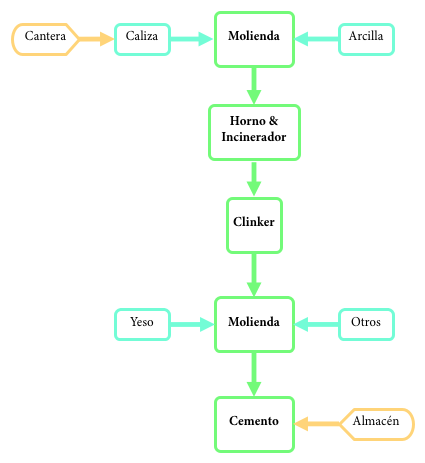
\includegraphics[width=15cm]{cemento.png}
\caption{Diagrama de flujo de la fabricación del cemento.}
\label{fig:cemento}
\end{figure}

Cuando se utiliza la palabra \emph{cemento} se refiere normalmente a un cemento tipo Portland (supone un 95\% de la producción de cementos \cite{jsjunnesson}), nombre no comercial que implica un proceso de producción y una composición característicos. De acuerdo a la norma UNE-EN 197-1:2011 \cite{une1971}, el cemento se divide en tres grupos en función de la cantidad de cemento Portland incluido: CEM I, CEM II y CEM III. El CEM I (95\% a 100\% de contenido de cemento Portland) es el más usado en la fabricación de adoquines.

Con respecto a la normativa específica de adoquines, la norma UNE 80301:1996 \cite{une80301} en el ámbito de España establece los requisitos que debe tener el cemento común. Si se utilizan cementos especiales se recurrirá a la norma UNE 80303:2013, y si son blancos a la norma UNE 80305:2012.

\subsection{Áridos}
Los áridos (entre los que se incluye la arena) son particulas de roca puede ser tanto gravas (piedras de forma natural) como macadán (piedras trituradas), teniendo cada tipo una textura diferente. Se pueden añadir diferentes tamaños de áridos para ejercer una función diferente según el mismo. Fracciones menores rellenarán las cavidades que haya entre partículas mayores, aportando adherencia a costa de un mayor peso.

El material de machaqueo para la producción de macadán se criba para eliminar las partículas menores. Debido a que las partículas que forman el macadán son más irregulares, es más fiable como material de relleno por su capacidad de incrustamiento (la grava tiene una forma más redondeada). El macadán se puede ser utilizado de forma más generalizada en función de la localización ya que la grava natural es un recurso más limitado.

La fuente de recursos de áridos son principalmente de río, mina o cantera o piedras trituradas (macadán). La granulometría de los áridos que se utilicen deberá cumplir las características indicada en la norma UNE EN 1338:2004/AC:2006.

\subsection{Agua}
El agua es muy importante en la constitución del hormigón. Reacciona químicamente con el cemento —hidratación— para proporcionar las propiedades deseadas del hormigón \cite{nrmca}. El agua de amasado es la cantidad de agua que toma contacto con el cemento y se usa para determinar las proporciones del resto de elementos para formar la mezcla. La fuerza y la durabilidad del cemento viene dado en gran parte por la cantidad de agua.

Además de su cantidad, la calidad del agua utilizada tiene efectos importantes en las propiedades del hormigón fresco, tales como el tiempo de fraguado y la facilidad de trabajo. También tiene importantes en la fuerza y durabilidad del hormigón endurecido.

\subsubsection{Fuentes posibles de agua}

Por norma general el agua adecuada para el consumo humano —agua potable— es válida. No obstante, el agua no potable puede ser utilizada siempre que no tenga un impacto negativo en las propiedades del hormigón. La mayoría de las plantas tienen una fuente de agua municipal que proporciona potable sin pruebas de calidad. En zonas rurales o en plantas portátiles in situ —instaladas y desinstaladas en el propio lugar del proyecto—, habrá que utilizar fuentes de agua no potable como ríos o masas de agua.

Otra fuente de agua es la reciclada de la limpieza —agua de lavado— de la mezcladora y otros elementos de la planta. También se podrá aprovechar el agua de precipitaciones atmosféricas que pueda recolectarse en las instalaciones de la planta.

El agua de procesado no sólo se genera de la fabricación del hormigón, sino también del lavado del hormigón reciclado. Los sistemas de recolección procesan el agua con el cemento y los áridos en forma de lechada que puede ser también utilizada como agua para la mezcla de hormigón.

Las normativas medioambientales suelen requerir que las plantas de fabricación traten y procesen tanto el agua de lluvia como el de procesado —agua de operaciones— para que adquiera ciertos niveles de pH y contenidos sólidos antes de que abandonen las instalaciones \cite{ermco}.

\subsubsection{Cualificación del agua no potable}
El agua es el recurso más importante para el ser humano. En algunas zonas el suministro de agua potable es muy escaso. El uso de fuentes de agua no potables para la producción de hormigón mantiene una producción sostenible de hormigón conservando los recursos de agua potable. La gestión del agua procedente de la producción de hormigón conforme con las normativas medioambientales representa un coste adicional para el fabricante, por lo que el uso de agua no potable representa un ahorro considerable en la producción de hormigón. Cuando se utilizan fuentes de agua no potable es importante verificar y documentar que las impurezas que contiene no merman las características del hormigón, ya que las fuentes pueden contener aceites, grasas, sales disueltas y otros elementos no controlados. Por esta razón, el fabricante debería tener en cuenta que su uso implica un coste adicional que evaluar y controlar.

\subsection{Aditivos}
Se podrán utilizar adiciones o aditivos siempre que produzcan el efecto deseado (acelerante, retardante,\ldots) y no afecte a las características esperadas del hormigón.

\section{Reciclado}
Cuando las construcciones de cemento se demuelen, el cemento es normalmente reutilizables \cite{jsjunnesson}. El cemento se transporta a una estación de reciclaje donde es triturado hasta un tamaño adecuado con la nueva utilización que se le va a dar. Puede ser empleado como material de relleno para el pavimento de nuevas carreteras o como árido en la producción de más cemento. La reutilización del cemento conlleva una disminución del uso de recursos naturales tales como la piedra o la grava.

HABLAR DEL CASO CONCRETO DE ADOQUINES Y SU RECICLADO (95\% se vuelven a usar para pavimentar. 30 años.)

%!TEX root = informe.tex
\chapter{Metodología del Análisis de Ciclo de Vida}
\section{Proceso completo}

Como se ha mencionado en la sección \ref{sec:introantecedentes}, el Análisis de Ciclo de Vida de un producto incluye todos los procesos de producción y servicios relacionados con el producto durante su ciclo de vida completo, desde la extracción de las materias primas hasta su reciclaje y/o disposición final, pasando por la fabricación y los subproductos que lo forman, la instalación, el uso y mantenimiento del producto. También se pueden incluir en las diferentes etapas del ciclo de vida el almacenamiento, venta, transporte y otras actividades que se consideren relevantes.

El Análisis de Ciclo de Vida hace distinción entre ``Entradas'' —materias primas, energía— y ``Salidas'' —emisiones a la tierra, mar o aire, desechos y subproductos.

DIAGRAMA INPUTS-OUTPUTS.

En las ``Entradas'' también pueden aparecer productos que proceden de la \textbf{tecnoesfera} —productos no naturales—, que añadirán su historial medioambiental a los cálculos del producto y/o servicio. Para el caso de residuos, se tendrán que incluir los futuros procesos de tratamiento.

El Análisis de Impacto del Ciclo de Vida (AICV) recoge la totalidad de entradas y salidas a la naturaleza para realizar un estudio potencial de los efectos medioambientales relacionados con el producto \cite{iso14040}.

DIAGRAMA LCIA + LCI + LCIA

\subsection{Etapas del Análisis de Ciclo de Vida}
\subsubsection{Definición de objetivos y alcance}
\subsubsection{Análisis de inventario (ICV)}
\subsubsection{Evaluación del impacto ambiental (EICV)}
\subsubsection{Interpretación}

\subsection{Ventajas e inconvenientes del ACV}

El Análisis de Ciclo de Vida es una herramienta que ofrece muchas ventajas:
\begin{itemize}
  \item el ACV es la única herramienta que examina los impactos medioambientales de un producto y/o servicio a través de su ciclo de vida.
  \item el ACV es un método estándar ISO.
  \item el ACV proporciona una visualización fácil de entender de separando en etapas las fuentes de impacto.
  \item el ACV puede tanto guiar las decisiones de un fabricante (nivel microeconómico) como ayudar a un gobierno a definir una política de actuación (nivel macroeconómico).
  \item el ACV distingue entre la información relevante mediante cuantificación objetiva y los asuntos que pertenecen a políticas y elecciones sociales.
\end{itemize}

Por otro lado, el Análisis de Ciclo de Vida tiene ciertas limitaciones:
\begin{itemize}
  \item los resultados son geográficamente dependientes. Los resultados de un estudio en Europa no son aplicable en Estados Unidos sin tener en cuenta las variaciones geográficas correspondientes (por ejemplo, el mix eléctrico).
  \item el ACV sólo evalúa los impactos potenciales, no los verdaderos impactos, por lo que no proporciona ninguna información de las consecuencias.
  \item los resultados de dos ACVs para un mismo objeto de estudio puede diferir según los objetivos, procesos, calidad de los datos y el método de análisis de impacto utilizados. La ISO insiste en transparencia a la hora de realizar un ACV.
  \item un ACV detallado requiere un inventario de todos los procesos elementales incluidos dentro de los parámetros del sistema.
  \item se requiere el uso de bases de datos, software especializado y personas capacitadas para poder analizar los datos.
\end{itemize}

\section{Bases de datos}

La calidad de los datos que aparecen en el Inventario de Ciclo de Vida (ICV) tienen gran importancia en la relevancia del estudio que se realice. En función de la base de datos utilizada el Análisis de Ciclo de Vida puede obtener resultados diferentes.

La metodología de uso del software de Análisis de Ciclo de Vida consiste en utilizar una base de datos como soporte para aquellos materiales y procesos de nuestro sistema que sean similares con los de la base de datos. En caso de que no se adapten a la entrada de la base de datos será necesario modelar una nueva entrada equivalente, pudiendo usar otras entradas de la base de datos.

Cuando se habla de bases de datos (BBDD) en el marco de un ACV, se pueden diferenciar, en función de los datos que contengan, dos tipos:
\begin{itemize}
  \item BBDD con las entradas/salidas que se emplean para simular el sistema analizado en el Inventario de Ciclo de Vida (ICV), conocidas como BBDD de ICV.
  \item BBDD con los datos que cada metodología de Evaluación de Impacto del Ciclo de Vida (EICV) necesita para que la herramienta que llevará a cabo el EICV haga los calculos, conocidas como BBDD de metodologías.
\end{itemize}

Las bases de datos de Inventarios de Ciclo de Vida (ICVs) están formadas por datos de muy diversos materiales y procesos, normalmente agrupados según la fase del ciclo de vida a la que hagan referencia. A través de ellas se puede asignar a cada entrada/salida reflejadas en el ICV una serie de información de la base de datos que indicará la información sobre su impacto ambiental, los factores de caracterización, normalización, etc \cite{ihobecarbono}.

Las bases de datos de metodologías están formadas por los factores de caracterización, ponderación y otros datos que cada metodología de EICV necesita para realizar los cálculos de obtención de resultados. Estas bases de datos recogen los datos en un formato estándar y común (ISO/TS 14048:2002), para que el software de Análisis de Ciclo de Vida pueden utilizar estos datos \cite{ihobecarbono}.

SimaPro (ver sección \ref{sec:simapro}) incorpora varias bases de datos de Inventarios de Ciclo de Vida:
\begin{itemize}
  \item ecoinvent (2009): más de 4000 procesos en energía, transporte, materiales; incluye construcción, químicos, agricultura, etc.; unidad y procesos de sistema.
  \item BUWAL 250 (1997): materiales generales, energía, transporte y desechos, parcialmente basada en base de datos ETH.
  \item ETH-ESU (1996): reconocida base de datos de energía y transporte.
  \item USA Input Output (2003): datos Entrada/Salida para los EE.UU.
  \item Industry data (2001): datos publicados por asociaciones industriales, como APME.
  \item Idemat (2001): base de datos holandesa, recopilada de diferentes fuentes.
  \item Franklin (1996): base de datos generales de EE.UU. sobre materiales, transporte y energía.
  \item Danish IO y Danish Food (2003): bases de datos de Dinamarca de Entrada/Salida y comida.
\end{itemize}

Entre las bases de datos de metodologías de Evaluación de Impactos de Ciclo de Vida, SimaPro incorpora las siguientes:
\begin{itemize}
  \item Efecto 2002: estimación de daños; muchas similitudes con Eco-indicador 99, pero con factores de toxicidad recalculados.
  \item TRACI 2002: método Midpoint desarrollado por US EPA.
  \item CML 2 baseline 2000: actualización del método de 1992, modelos re- avanzados e inclusión de análisis de destino.
  \item EPS 2000: Estimación de daños, usando monetarización (intención de pagar) en lugar de peso por un panel. No hay necesidad de normalización en esta estimación.
  \item Eco-indicator 99: estimación de daños; usa indicadores de categoría en el nivel final. Se incluyen tres versiones usando diferentes suposiciones en los modelos medioambientales.
  \item Ecopoints 97 (UBP): distancia al objetivo basado en objetivos de políticas suizas (conocido también como método de escasez o UBP).
  \item EDIP 97: método de caracterización y normalización desarrollado por EPA de Dinamarca.
  \item Eco-indicator 95: distancia al método objeto basado en objetivos científicos e incluye estimación de daños.
  \item CML 92: método “midpoint” (punto intermedio) bastante usado, caracterización relativamente simple, sin destino o exposición, varios sets de normalización.
\end{itemize}

\subsubsection{ecoinvent}

\textit{ecoinvent} implementa en una única base de datos miles de conjuntos de datos de ICVs —agricultura, energía, transporte, combustibles, biomateriales, químicos, materiales de construcción, materiales de empaquetamiento, metales elementales y preciosos, procesado de metales, informática y electrónica, tratamiento de residuos— basados en información industrial recopilada por grupos de investigación y consultores reconocidos internacionalmente \cite{website:ecoinvent}.

\begin{figure}[!htb]
\centering
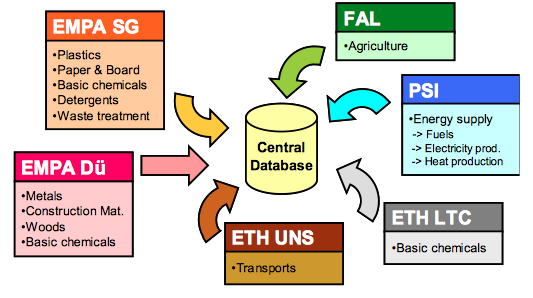
\includegraphics[width=13cm]{bbddecoinvent.png}
\caption[Estructura de la base de datos de \textit{ecoinvent}.]{Estructura de la base de datos de \textit{ecoinvent}. Fuente: \protect\cite{mgoedkoop2}.}
\label{fig:bbddecoinvent}
\end{figure}

La base de datos \textit{ecoinvent}:
\begin{itemize}
  \item Incorpora más de 4000 procesos:
  \begin{itemize}
    \item Bienes de producción y calidades.
    \item Para algunos procesos añade diferencias regionales (Suiza y Unión Europea).
    \item Mix eléctrico y procesos agrícolas de Estados Unidos y Asia.
  \end{itemize}
  \item Incertidumbre en los datos.
  \item Ilustraciones de la mayoría de los procesos.
  \item Documentación extensa y consistente de los procesos.
  \item Actualizaciones frecuentes y periódicas.
  \item Incluye versiones de los procesos como Unidad (Proceso 1/U) —más detallado— o como Sistema (Proceso 1/S) —sin información de incertidumbre—.
\end{itemize}

\section{Software de análisis}

El mercado ofrece una amplia gama de programas para el Análisis de Ciclo de Vida que ofrecen diferentes tipos de prestaciones y rangos de precios. Entre ellos cabe destacar:

\begin{itemize}
  \item SimaPro: ver sección \ref{sec:simapro}.
  \item Gabi: permite esbozar ideas en su interfaz y ofrece un potente asistencia para la creación del inventario. Incorpora una base de datos propietaria que también funciona con \textit{ecoinvent}. Es compatible con los estándares ISO 14040 y bastante flexible.
  \item Quantis Suite: facilita el acceso a personas no expertas con plantillas y asistentes. Incorpora una base de datos propia.
  \item EarthSmart: permite crear inventarios de forma rápida aunque el usuario no sea experto. Permite crear un final de vida basado en escenarios creados por expertos. Incorpora varias bases de datos como \textit{ecoinvent} y la Australian LCI database.
  \item Eco-it: desarrollada para la Sociedad Pública de Gestión Ambiental del País Vasco (IHOBE). Realiza Análisis de Ciclo de Vida simplificado basado en la metodología ReCiPe, así como Huella de Carbono basado en valores IPCC. Es compatible con la normativa ISO 14040.
  \item openLCA: es una aplicación profesional de código abierto y gratuita para Análisis de Ciclo de Vida y Huella de Carbono creada por GreenDelta.
\end{itemize}

El paquete de software utilizado para este proyecto será SimaPro debido a la versatilidad que aporta, disponibilidad, inclusión de base de datos \textit{ecoinvent} y su compatibilidad con la norma ISO 14040.

\subsection{SimaPro}\label{sec:simapro}
SimaPro es una herramienta profesional desarrollada por la empresa holandesa PRé Consultants para el Análisis de Ciclo de Vida más utilizada actualmente por la mayor parte de los consultores y la industria, apoyada en la investigación de materiales y elementos por parte institutos y universidades \cite{mgoedkoop}. Permite modelar ciclos de vida complejos y analizarlos de forma sistemática y transparente, ya que puede rastrearse el origen de todos los resultados de forma sencilla.

\begin{figure}[!htb]
\centering
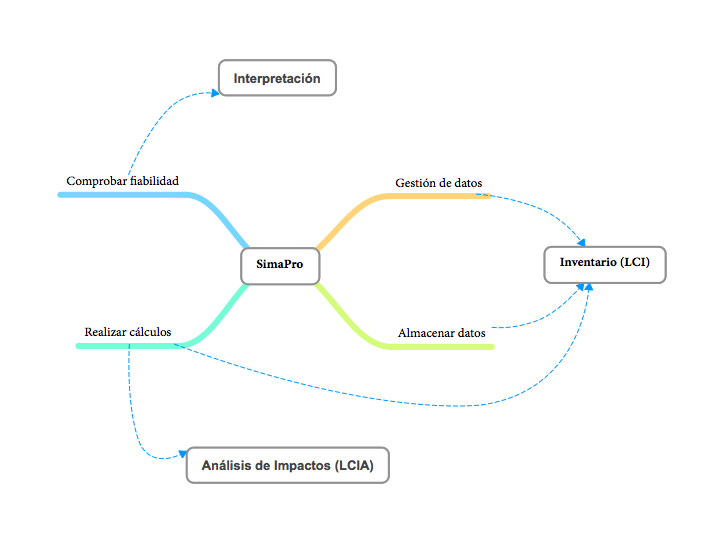
\includegraphics[width=13cm]{simapro.png}
\caption{Estructura de SimaPro.}
\label{fig:simapro}
\end{figure}

Entre sus principales cualidades destacan:

\begin{itemize}
  \item Diseño de productos.
  \item Desarrollo de indicadores clave.
  \item Cálculo de la huella de carbono de muchos tipos de productos y sistemas.
  \item Determinar el impacto medioambiental de productos o servicios con precisión estadística mediante el método de análisis Monte Carlo.
  \item Incluye Declaraciones Medioambientales de Productos e Informes Medioambientales GRI (Global Reporting Initiative).
  \item Utilización de bases de datos con inventarios.
  \item Asignación de múltiples procesos de salida.
  \item Análisis de Punto Débil, que permite identifica los puntos sensibles en el ciclo de vida utilizando un árbol de procesos.
  \item Análisis de tratamientos de residuos y escenarios de reciclado.
\end{itemize}

Esta herramienta cuenta con una interfaz de usuario intuitiva con un explorador de guía a través del Análisis de Ciclo de Vida del producto o servicio siguiendo los principios de las normas ISO 14040 y 14044. Además incorpora un modelado utilizando un asistente paso a paso.

La mayor ventaja de esta herramienta es la utilización de bases de datos con los inventarios de miles de procesos y métodos más importante de análisis de impacto.

SimaPro incluye varias bases de datos de inventarios con miles de procesos, además de los métodos de análisis de impacto más importantes. De esta forma, no es necesario recolectar datos de procesos individuales y poder centrarse en los asuntos más importantes del estudio.

\begin{figure}[!htb]
\centering
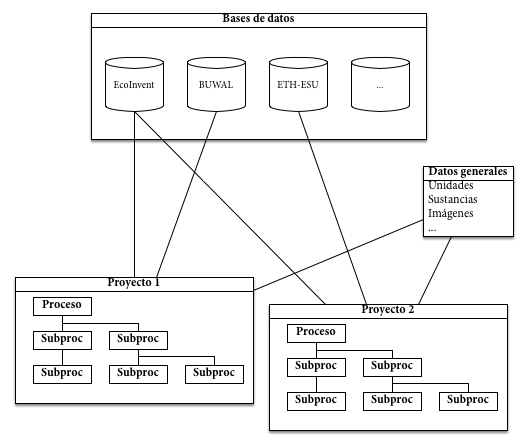
\includegraphics[width=15cm]{bbddsimapro.png}
\caption{Estructura de una base de datos de SimaPro.}
\label{fig:bbddsimapro}
\end{figure}

\section{Metodología para Evaluación del Impacto del Ciclo de Vida}

XXX Comprobar título y si ecoinvent tiene recipe ipcc etc (ver su manual)

La base de datos \textit{ecoinvent} ofrece múltiples métodos para la evaluación de impactos que aplican diferentes factores —caracterización, normalización, peso y daño— a cada flujo elemental de la tabla de inventario según su implementación. Los métodos más destacables que se tendrán en cuenta en este proyecto son:

\begin{itemize}
  \item Método ReCiPe: categorías de impacto y áreas de protección del medio ambiente.
  \item Método de Demanda de Energía Acumulada: cuantificación de energía consumida.
  \item Método IPCC 2007: cálculo potencial del calentamiento global a lo largo del ciclo de vida.
\end{itemize}

\subsection{ReCiPe}\label{sec:recipe}

El desarrollo de ReCiPe se debió al principio a integrar la metodología orientada al problema de \textit{CML-IA} y la metodología orientada al daño de \textit{Ecoindicator 99}. De esta manera, ReCiPe se convirtió en el sucesor de ambos métodos \cite{mgoedkoop3}.

La metodología orientada al problema de \textit{CML-IA} define las categorías de impacto en el punto medio. La incertidumbre de los resultado en este punto es relativamente baja. El inconveniente de este sistema es la ambigüedad de las conclusiones al haber demasiadas categorías de impacto.

La metogología orientada al daño de \textit{Ecoindicator 99} aborda sólo tres categorías de impacto, lo que hacer más fácil obtener conclusiones. Sin embargo, la incertidumbre de los resultados es más alta que con la otra metodología.

ReCiPe implemente ambas estrategias incluyendo las categorías de impacto tanto a punto medio como a punto final. A los factores de caracterización a punto medio se les aplica un factor de daño para obtener los valores de caracterización de punto final. ReCiPe comprende un total de 21 categorías de impacto agrupadas en 2 conjuntos (ver figura ref{recipecategoriasimpacto}):
\begin{itemize}
\item Punto medio: 18 categorías de impacto.
\item Punto final: 3 categorías de impacto.
\end{itemize}

\begin{figure}[!htb]
\centering
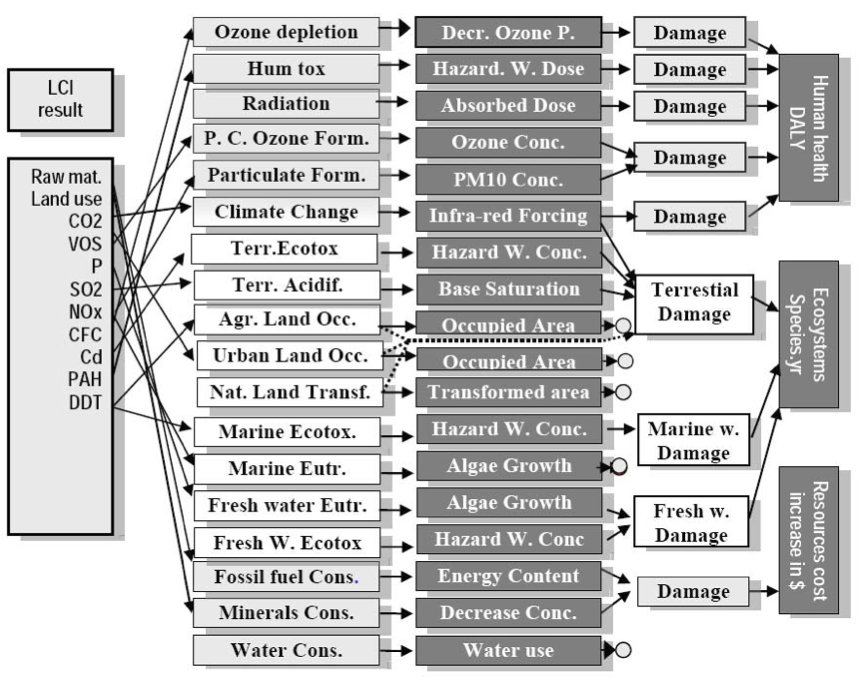
\includegraphics[width=12cm]{recipecategoriasimpacto.png}
\caption[Categorías de impacto aplicadas por ReCiPe.]{Categorías de impacto aplicadas por ReCiPe. Fuente: \protect\cite{mgoedkoop3}.}
\label{fig:recipecategoriasimpacto}
\end{figure}

\subsection{Demanda de Energía Acumulada}

Esta metodología —desarrollada a principio de los 70 debido a la crisis del petróleo— permite investigar el uso de energía a través del ciclo de vida de un producto o servicio. El análisis de la Demanda Acumulada de Energía consiste en la cuantificación tanto del uso directo como directo de energía —o consumo gris— durante todo el ciclo de vida del producto \cite{ecoinventlcia}.

Los valores CED (Cumulate Energy Demand) pueden utilizarse para comparar los resultado de un estudio detallada de Análisis de Ciclo de Vida con otros donde se indica únicamente la demanda de energía. También pueden utilizarse como indicador de verificación de los datos ya que es bastante fácil juzgar en base a la Demanda de Energía Acumulada si se han cometido errores importantes o no \cite{ecoinventlcia}.

Debido a que existe divergencias en los conceptos para la caracterización de las fuentes de energía primarias, los indicadores CED se dividen en ocho subcategorías para su uso con la base \textit{ecoinvent}, divididos en dos categorías base:

\begin{itemize}
  \item Fuentes no renovables: fósil, nuclear y bosque primario.
  \item Fuentes renovables: biomasa, viento, solar, geotérmica y agua.
\end{itemize}

\subsection{IPCC 2007}

El método IPCC 2007 —Intergovernmental Panel on Climate Change— es una actualización su homónimo de 2001. Este método es uno de los más empleados en la evaluación de impactos ya que realiza una caracterización de diferentes emisiones gaseosas de acuerdo a su Potencial de Calentamiento Global —Global Warming Potencial, GWP— y al conjunto de diferentes emisiones en la categoría de impacto de calentamiento global. Los valores de caracterización para las emisiones de gases de efecto invernadero se basan en los potenciales de calentamiento global publicados por el propio Grupo Intergubernamental de Expertos sobre el Cambio Climático (IPCC).

Al igual que en la versión de 2001, se establecen tres horizontes temporales para mostrar los efectos de la duración en la atmósfera de los diferentes gases:

\begin{itemize}
  \item GWP 20a (20 años).
  \item GWP 100a (100 años).
  \item GWP 500a (500 años).
\end{itemize}

Los Potenciales de Calentamiento Global (GWPs) directos están relacionados con el impacto del dióxido de carbono (\ce{CO2}). Los GWPs son un índice para la estimación de la contribución de calentamiento global relativo debido a las emisión atmosférica de un kilogramo de un gas de efecto invernadero concreto comparado con la emisión de un kilogramo de \ce{CO2} \cite{ecoinventlcia}.

\include{inventario}
%!TEX root = informe.tex
\chapter{Análisis de Ciclo de Vida: fabricación}
% Manual Euroadoquín. Documentos de Malaka.

\section{Introducción}\label{sec:obtenciondedatos}
Los datos de partida que se han utilizado en este análisis han sido proporcionados por Malaka de Prefabricados (Apéndice \ref{apend:datos}). La figura \ref{fig:diagrama_de_flujo} muestra las entradas al sistema, así como los procesos que ocurren durante la fabricación —que serán explicados en las siguientes secciones— y la salida del sistema.

\begin{figure}[!htb]
\centering
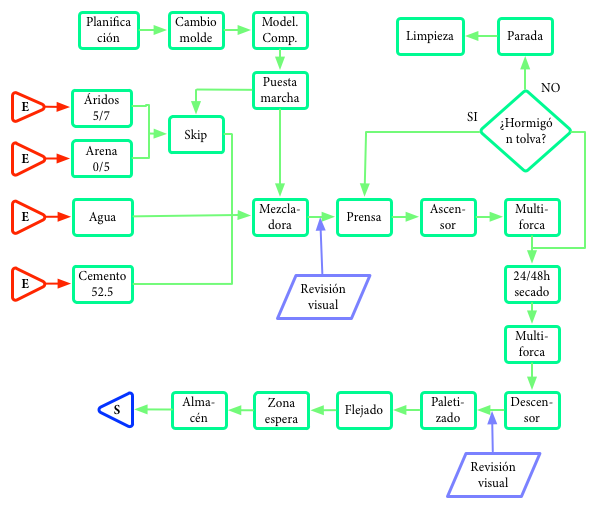
\includegraphics[width=15cm]{diagrama.png}
\caption{Diagrama de flujo de la fabricación de adoquines.}
\label{fig:diagrama_de_flujo}
\end{figure}

En primer lugar es necesario señalar que el modelo de adoquín ``Holanda 6'', cuya hoja de datos técnicos aparece en el Apéndice \ref{apend:catalogo}, es el que mayor demanda de fabricación tiene en la empresa, por lo que se ha dispuesto de mayor número de datos.

Cada bandeja fabricada supone exactamente 0.5 \si{m^2} de adoquines modelo ``Holanda 6''. Como se ha tomado como Unidad Funcional 1 \si{m^2} de adoquín, los cálculos se han realizado para 2 bandejas. Cada adoquín mide 200x100x60 \si{mm} y pesa 3 \si{kg}. Como cada bandeja está formada por 25 adoquines, y son necesarias 2 bandejas para tener 1 \si{m^2}, se tiene un total de 50 adoquines/\si{m^2} (ecuación \ref{eq:masa}). De esta forma:

\begin{gather}
200 mm \times 100 mm \times 25 ud/bandeja \times 2 bandeja = 1 m^2\\
3 kg/ud \times 50 ud/m^2 = 150 kg/m^2 \text{ de masa para adoquín}\label{eq:masa}
\end{gather}

Como es necesario disponer de 150 \si{kg/m^2} de masa para adoquín, se aplican los porcentajes de materias primas sobre la fórmula base para adoquín ``Holanda 6'' para obtener las masas de cada materia prima reflejadas en la tabla \ref{desglosemateriasprimas}.

\begin{table}[!htb]
\centering
\begin{tabular}{lcccc}
\toprule
\multicolumn{5}{c}{Consumo de materias primas por \si{m^2} de adoquín fabricado}\\
\midrule
Materia prima & \% Fórmula & Masa (\si{kg}) & Proced. & Dist. (\si{km})\\
\midrule
Árido tipo 5/7 & 37.75 & 56.63 & Alh. Torre & 8\\
Arena tipo 0/5 & 47.16 & 70.74 & Alh. Torre & 8\\
Cemento Portland 52.5N & 10.06 & 15.09 & Málaga-El Palo & 30\\
Agua & 5.03 & 7.54 & Red & -\\
\bottomrule
\end{tabular}
\caption{Desglose de materias primas por \si{m^2} de adoquín fabricado.}
\label{desglosemateriasprimas}
\end{table}

En el Apéndice \ref{apend:catalogo} también se especifica un diagrama de Gantt de los procesos para una simulación realizada para fabricar 1 \si{m^2} de adoquín, además de los consumos energéticos desglosados.

\section{Modelado de los procesos}\label{sec:modeladoprocesos}
\subsection{Cemento}
El cemento se transporta a granel en camiones con tanques a presión hasta la fábrica. Allí se almacena en silos provistos de compresores que descargan el material desde el tanque hasta su interior. El compresor es alimentado por electricidad mediante una toma de corriente conectada a la red eléctrica. La descarga del silo es únicamente por gravedad con válvulas dosificadoras de control de caudal (ver tabla \ref{modeladodelcemento}).

Las unidades para el modelado del camión (lorry) vienen expresadas en \si{kg\times km}, mientras que el uso del silo se proporciona en \si{m^3}, dada una densidad media del cemento Portland de 1250 \si{kg/m3} \cite{website:ecoinvent}.

\begin{gather}
15.09 kg \times 30 km = 453 kg\times km\\
15,09 kg / 1250 kg/m^3 = 0.0121 m^3
\end{gather}

El mix eléctrico se obtiene del consumo del compresor del silo proporcional a una cantidad de 15.09 \si{kg}, si la potencia del compresor son 30kW, velocidad de carga del silo es 35 \si{\tonne/h} para un tiempo de llenado de 35 minutos.

\begin{gather}
30 kW \times 1 h \times \frac{35 min}{60 min} = 17.5 kWh = 63 MJ \text{ para 20 toneladas}\\
35 t/h \times \frac{35 min}{60 min} = 20 t \text{ de cemento con el silo cargado}\\
15.09 kg \times \frac{63 MJ}{20 t} = 4.79 kJ
\end{gather}

\begin{table}[!htb]
\centering
\begin{tabular}{p{8cm}rc}
\toprule
\multicolumn{3}{c}{Cemento Portland CEM I 52.5Z gris}\\
\midrule
Materiales/Ensamblajes & Cantidad & Unidad\\
\midrule
Portland cement, strength class Z 52.5, at plant/CH U & 15.09 & \si{kg}\\
\midrule
Procesos & Cantidad & Unidad\\
\midrule
Transport, lorry 16-32t, EURO4/RER U & 453 & \si{kg*km}\\
Tower silo, plastic/CH/I U & 0.0121 & \si{m^3}\\
Electricity mix 2013/ES U & 4.79 & \si{kJ}\\
\bottomrule
\end{tabular}
\caption{Modelado del cemento.}
\label{modeladodelcemento}
\end{table}

\subsection{Arena y áridos}
Las arenas y áridos se transportan hasta la planta de fabricación mediante camiones. Actualmente los áridos y la arena ya no se apilan a bajo techados en las explanadas adyacentes a las plantas, sino que el propio transporte rellena las tolvas de forma automática.

El tipo de arena que se utiliza en la planta es 0/5 —granulometría en milímetros de las partículas que forman la arena— no está directamente disponible en SimaPro. En su lugar, se ha optado por tomar el material ``Sand 0/2'' (Arena tipo 0/2), que además de pertenecer a la clasificación general de arena —de 0 a 5 \si{mm}—, la descripción de SimaPro indica que puede utilizarse como árido natural estándar en la industria de la construcción (ver tabla \ref{modeladodelaarena}).

\begin{quote}
Technical purpose of product or process: Standard mineral product used as natural aggregates in the construction industry according to the applied technology.
\end{quote}

Las unidades para el modelado del camión (lorry) vienen expresadas en \si{kg\times km}.

\begin{equation}
70.74 kg \times 8 km = 566 kg\times km
\end{equation}

\begin{table}[!htb]
\centering
\begin{tabular}{p{8cm}rc}
\toprule
\multicolumn{3}{c}{Arena tipo 0/5}\\
\midrule
Materiales/Ensamblajes & Cantidad & Unidad\\
\midrule
Sand 0/2, wet and dry quarry, production mix, at plant, undried/RER S & 70.74 & \si{kg}\\
\midrule
Procesos & Cantidad & Unidad\\
\midrule
Transport, lorry 16-32t, EURO4/RER U & 566 & \si{kg*km}\\
\bottomrule
\end{tabular}
\caption{Modelado de la arena.}
\label{modeladodelaarena}
\end{table}

Los áridos utilizados para producir adoquines puede incluir arena, gravilla y piedra de machaqueo si se pretende obtener un producto de peso normal. Si se desea que el adoquín sea más ligero —entre un 20 y un 45 \%— sin mermar sus propiedades estructurales se utilizan materiales como pizarra, arcilla, escoria de altos hornos y cenizas de carbón según su disponibilidad y coste.

El tipo de árido utilizado en planta es de granulometría 5/7 —en milímetros—, catalogado como gravilla. No está directamente disponible en SimaPro, por lo que en su lugar, se ha optado por tomar el material ``Gravel, crushed'' (gravilla de machaqueo) (tabla \ref{modeladodearido}).

Las unidades para el modelado del camión (lorry) vienen expresadas en \si{kg\times km}.

\begin{equation}
56.63 kg \times 8 km = 566 kg\times km
\end{equation}

\begin{table}[!htb]
\centering
\begin{tabular}{p{8cm}rc}
\toprule
\multicolumn{3}{c}{Árido tipo 5/7}\\
\midrule
Materiales/Ensamblajes & Cantidad & Unidad\\
\midrule
Gravel, crushed, at mine/CH U & 56.63 & \si{kg}\\
\midrule
Procesos & Cantidad & Unidad\\
\midrule
Transport, lorry 16-32t, EURO4/RER U & 453 & \si{kg*km}\\
\bottomrule
\end{tabular}
\caption{Modelado del árido.}
\label{modeladodearido}
\end{table}


\subsection{Agua}
La mayoría de las plantas tienen una fuente de agua municipal (\textit{tap water}) que proporciona potable perfectamente válida para el uso en la fabricación de hormigón (ver tabla \ref{modeladodelagua}).

\begin{table}[!htb]
\centering
\begin{tabular}{p{8cm}rc}
\toprule
\multicolumn{3}{c}{Agua}\\
\midrule
Materiales/Ensamblajes & Cantidad & Unidad\\
\midrule
Tap water, at user/RER U & 7.54 & \si{kg}\\
\bottomrule
\end{tabular}
\caption{Modelado del agua.}
\label{modeladodelagua}
\end{table}

\subsection{Dosificador de arena y áridos}

El sistema de control central manda una señal a los dosificadores para que viertan la cantidad ordenada por el programa principal de fabricación. Dichos dosificadores consisten en una especie de tolva con forma de embudo con un cierre controlado por el sistema.

No existe un modelo de referencia en SimaPro para este tipo de dosificadores —\textit{feed hopper}, en inglés—, por lo que se ha simplificado un modelo válido \cite{woodpellet}. Se le ha añadido la parte de mix eléctrico de los datos del fabricante (Apéndice \ref{apend:datos}). El dosificador del cemento y del agua están incluidos en su propio modelo (silo y abastecimiento de la red respectivamente).

\begin{table}[!htb]
\centering
\begin{tabular}{p{8cm}rc}
\toprule
\multicolumn{3}{c}{Dosificadores para arena y áridos}\\
\midrule
Materiales/combustibles & Cantidad & Unidad\\
\midrule
Steel, low-alloyed, at plant/RER U & 47 & \si{kg}\\
\midrule
Electricidad/calor & Cantidad & Unidad\\
\midrule
Electricity mix 2013/ES U & 0.0021 & \si{MJ}\\
\bottomrule
\end{tabular}
\caption{Modelado de los dosificadores para arena y áridos.}
\label{modeladodedosificadores}
\end{table}

\subsection{Cintas transportadoras de áridos y cemento}

Las tolvas descargan la cantidad programada de materia prima sobre dos cintas transportadoras —una para áridos y arena, otra para cemento— con básculas de pesaje incorporadas que se comunican con el sistema de control y cortan el flujo de descarga.

La cinta de áridos descarga sobre un skip que eleva los materiales hasta una mezcladora. La cinta de cemento descarga directamente sobre la mezcladora.

Las distancias están medidas sobre planos (Apéndice \ref{apend:planos}), y los consumos se han obtenido de los ensayos en fábrica a partir de la potencia de la cinta transportadora y el tiempo de funcionamiento (Potencia=Energía/Tiempo).

\begin{table}[!htb]
\centering
\begin{tabular}{p{8cm}rc}
\toprule
\multicolumn{3}{c}{Cinta transportadora para arena y áridos}\\
\midrule
Materiales/combustibles & Cantidad & Unidad\\
\midrule
Conveyor belt, at plant/RER/I U & 14.6 & \si{m}\\
\midrule
Electricidad/calor & Cantidad & Unidad\\
\midrule
Electricity mix 2013/ES U & 0.1827 & \si{MJ}\\
\bottomrule
\end{tabular}
\caption{Modelado de la cinta transportadora para arena y áridos.}
\label{modeladodecintaarena}
\end{table}

\begin{table}[!htb]
\centering
\begin{tabular}{p{8cm}rc}
\toprule
\multicolumn{3}{c}{Cinta transportadora para cemento}\\
\midrule
Materiales/combustibles & Cantidad & Unidad\\
\midrule
Conveyor belt, at plant/RER/I U & 7.3 & \si{m}\\
\midrule
Electricidad/calor & Cantidad & Unidad\\
\midrule
Electricity mix 2013/ES U & 0.0975 & \si{MJ}\\
\bottomrule
\end{tabular}
\caption{Modelado de la cinta transportadora para cemento.}
\label{modeladodecintacemento}
\end{table}

\subsection{Skip y mezcladora}

Para asegurar la consistencia del lote el agua se añade mediante un sistema electrónico de control que dosifica el caudal. En el caso de que haya otros aditivos, tales como acelerantes o colorantes, es en este momento cuando se incorporan a la mezcla. Cuando se termina de añadir el agua se produce el mezclado creando hormigón fresco.

La base de datos \textit{ecoinvent} proporciona un modelo para el mezclado del hormigón, ``Paster mixing'' en el que se introduce la masa de la mezcla, 150 \si{kg} y al que se le añade la parte de mix eléctrico de los datos del fabricante (Apéndice \ref{apend:datos}).

\begin{table}[!htb]
\centering
\begin{tabular}{p{8cm}rc}
\toprule
\multicolumn{3}{c}{Skip y mezcladora}\\
\midrule
Materiales/combustibles & Cantidad & Unidad\\
\midrule
Plaster mixing/CH U & 150 & \si{kg}\\
\midrule
Electricidad/calor & Cantidad & Unidad\\
\midrule
Electricity mix 2013/ES U & 1.71 & \si{MJ}\\
\bottomrule
\end{tabular}
\caption{Modelado del skip y la mezcladora.}
\label{modeladoskip}
\end{table}

\subsection{Cinta transportadora para hormigón}

El hormigón sale de la mezcladora mediante una cinta transportadora que contiene otra báscula de pesaje y se dirige hacia la tolva de hormigón que se encuentra en lo alto de la prensa.

La base de datos \textit{ecoinvent} proporciona un modelo para la cinta transportadora, ``Conveyor belt'' en el que se introduce la distancia de recorrido, 12.1 \si{m}, y al que se le añade la parte de mix eléctrico de los datos del fabricante (Apéndice \ref{apend:datos}).

\begin{table}[!htb]
\centering
\begin{tabular}{p{8cm}rc}
\toprule
\multicolumn{3}{c}{Cinta transportadora para hormigón}\\
\midrule
Materiales/combustibles & Cantidad & Unidad\\
\midrule
Conveyor belt, at plant/RER/I U & 12.1 & \si{m}\\
\midrule
Electricidad/calor & Cantidad & Unidad\\
\midrule
Electricity mix 2013/ES U & 0.088 & \si{MJ}\\
\bottomrule
\end{tabular}
\caption{Modelado de la cinta transportadora para hormigón.}
\label{modeladodecintahormigon}
\end{table}

\subsection{Tolva para hormigón}

La tolva de hormigón se encarga de dosificar el hormigón en el molde de la prensa. No existe un modelo de referencia en SimaPro para tolvas —\textit{hopper}, en inglés—, por lo que se ha simplificado un modelo válido \cite{foodnottrash}. Se le ha añadido la parte de mix eléctrico de los datos del fabricante (Apéndice \ref{apend:datos}).

\begin{table}[!htb]
\centering
\begin{tabular}{p{8cm}rc}
\toprule
\multicolumn{3}{c}{Tolva para hormigón}\\
\midrule
Materiales/combustibles & Cantidad & Unidad\\
\midrule
Steel, low-alloyed, at plant/RER U & 470 & \si{kg}\\
\midrule
Electricidad/calor & Cantidad & Unidad\\
\midrule
Electricity mix 2013/ES U & 0.0161 & \si{MJ}\\
\bottomrule
\end{tabular}
\caption{Modelado de la tolva para hormigón.}
\label{modeladotolvahormigon}
\end{table}

\subsection{Vibrocompresión}

La tolva dosifica el hormigón fresco, que cae en los moldes para adoquines. Los moldes tienen una longevidad muy alta —aproximadamente un millón de ciclos de prensado— y su durabilidad depende de las propiedades abrasivas de los áridos utilizados.

El molde se compone de dos partes: la parte donde se inyecta el hormigón (hembra) y la parte que se coloca encima para dar forma (macho). La prensa tiene incorporado un carro alimentador encargado de proporcionar la parte hembra. Se inyecta el hormigón en el molde hembra, el molde macho baja con la prensa y el hormigón es compactado y cimentado usando un sistema combinado de presión y vibración. Cada molde puede producir 25 adoquines de 200x100x60\si{\milli\meter}, lo que proporciona a una superficie adoquinada de 0.5\si{\square\meter}. Los adoquines son moldeados de una sola pieza y extraidos del molde inmediatamente después de la vibro-compresión sobre una bandeja de madera.

SimaPro no proporciona un modelo para prensas de cemento. Estudiando las similitudes entre una planta de hormigón —\textit{concrete plant}— y la planta objeto de este proyecto, se puede aproximar un modelo de la prensa basado en la maquinaria del primero \cite{buildingproducts}. La aproximación ``Industrial machine, heavy, unspecified, at plant'' pide la masa de la máquina industrial no específica que realiza el proceso. De acuerdo al fabricante, ese dato es de 1380 \si{kg}, al que se le ha añadido la parte de mix eléctrico también proporcionado por el fabricante (Apéndice \ref{apend:datos}).

\begin{table}[!htb]
\centering
\begin{tabular}{p{8cm}rc}
\toprule
\multicolumn{3}{c}{Prensado}\\
\midrule
Materiales/combustibles & Cantidad & Unidad\\
\midrule
Industrial machine, heavy, unspecified, at plant/RER/I U & 9000 & \si{kg}\\
\midrule
Electricidad/calor & Cantidad & Unidad\\
\midrule
Electricity mix 2013/ES U & 0.437 & \si{MJ}\\
\bottomrule
\end{tabular}
\caption{Modelado del prensado.}
\label{modeladoprensado}
\end{table}

\subsection{Cinta transportadora para piezas frescas}

La bandeja con las piezas frescas es trasladada sobre un transportador de rodillos hasta un ascensor.

SimaPro no proporciona un modelo para este tipo de transportador. Estudiando las similitudes entre un transportador de rodillos y una cinta transportadora se puede aproximar un modelo propio basado en que la principal diferencia es la falta de una banda de rodadura (tabla \ref{modeladotransportadorrodillos}).

\begin{table}[!htb]
\centering
\begin{tabular}{p{8cm}rc}
\toprule
\multicolumn{3}{c}{Transportadora de rodillos para piezas frescas}\\
\midrule
Materiales/combustibles & Cantidad & Unidad\\
\midrule
Concrete, sole plate and foundation, at plant/CH U & 0.01 & \si{m^3}\\
Section bar rolling, steel/RER U & 500 & \si{kg}\\
Steel, low-alloyed, at plant/RER U & 530 & \si{kg}\\
Transport, lorry >16t, fleet average/RER U & 55.5 & \si{\tonne\times km}\\
Wire drawing, steel/RER U & 29.6 & \si{kg}\\
\midrule
Residuos y emisiones para tratamiento & Cantidad & Unidad\\
\midrule
Disposal, building, reinforced concrete, to final disposal/CH U & 23 & \si{kg}\\
Disposal, steel, 0\% water, to municipal incineration/CH U & 29.6 & \si{kg}\\
\bottomrule
\end{tabular}
\caption{Modelado de 1 metro de transportador de rodillos.}
\label{modeladotransportadorrodillos}
\end{table}

La aproximación ``Roller conveyor, at plant'' pide como parámetro la distancia de recorrido, 6.8 \si{m}, al que se le ha añadido la parte de mix eléctrico también proporcionado por el fabricante (Apéndice \ref{apend:datos}).

\begin{table}[!htb]
\centering
\begin{tabular}{p{8cm}rc}
\toprule
\multicolumn{3}{c}{Transportadora de rodillos para piezas frescas}\\
\midrule
Materiales/combustibles & Cantidad & Unidad\\
\midrule
Conveyor belt, at plant/RER/I U & 6.8 & \si{m}\\
\midrule
Electricidad/calor & Cantidad & Unidad\\
\midrule
Electricity mix 2013/ES U & 0.077 & \si{MJ}\\
\bottomrule
\end{tabular}
\caption{Modelado del transportador de rodillos para piezas frescas.}
\label{modeladotransportadorpiezas}
\end{table}

\subsection{Ascensor}

Este ascensor tiene diez alturas, de forma que cada vez que recibe una bandeja con adoquines frescos, la bandeja anterior sube una altura y monta la siguiente. El ascensor se encarga de alimentar un carro multiforca de diez alturas.

SimaPro no proporciona un modelo para un ascensor de estas características, por lo que se ha obtado por un elemento genérico que sí esté en la base de datos de \textit{ecoinvent} como ``Industrial machine, heavy, unspecified, at plant'' que pide la masa de la máquina industrial no específica que realiza el proceso. De acuerdo al fabricante, ese dato es de 320 \si{kg}, al que se le ha añadido la parte de mix eléctrico también proporcionado por el fabricante (Apéndice \ref{apend:datos}).

\begin{table}[!htb]
\centering
\begin{tabular}{p{8cm}rc}
\toprule
\multicolumn{3}{c}{Ascensor}\\
\midrule
Materiales/combustibles & Cantidad & Unidad\\
\midrule
Industrial machine, heavy, unspecified, at plant/RER/I U & 320 & \si{kg}\\
\midrule
Electricidad/calor & Cantidad & Unidad\\
\midrule
Electricity mix 2013/ES U & 0.126 & \si{MJ}\\
\bottomrule
\end{tabular}
\caption{Modelado del ascensor.}
\label{modeladodelascensor}
\end{table}

\subsection{Multiforca}
Cuando las diez alturas está ocupadas se cargan en un carro multiforca —\textit{rack transporter}, en inglés— automatizado que transporta las piezas hasta un secadero.

Las piezas permanecen en el secadero curándose a temperatura ambiente entre 24 y 48 horas.

Una vez transcurrido el tiempo de curado, los adoquines están secos y listos para ser recogidos por otro carro multiforca automatizado que recoge las bandejas y las lleva a un descensor.

SimaPro tampoco proporciona un modelo para un carro multiforca, por lo que también se ha obtado por un elemento genérico que sí esté en la base de datos de \textit{ecoinvent} como ``Industrial machine, heavy, unspecified, at plant'' que pide la masa de la máquina industrial no específica que realiza el proceso. De acuerdo al fabricante, un carro multiforca se compone de un tres partes: transportador de forca (rackveyor), rodadura (crawler) y vehículo (transfer car), sumando en total 7500 \si{kg}, a lo que se le ha añadido la parte de mix eléctrico también proporcionado por el fabricante (Apéndice \ref{apend:datos}).

\begin{table}[!htb]
\centering
\begin{tabular}{p{8cm}rc}
\toprule
\multicolumn{3}{c}{Multiforca}\\
\midrule
Materiales/combustibles & Cantidad & Unidad\\
\midrule
Industrial machine, heavy, unspecified, at plant/RER/I U & 7500 & \si{kg}\\
\midrule
Electricidad/calor & Cantidad & Unidad\\
\midrule
Electricity mix 2013/ES U & 0.516 & \si{MJ}\\
\bottomrule
\end{tabular}
\caption{Modelado de la multiforca.}
\label{modeladomultiforca}
\end{table}

\subsection{Descensor}
El descensor coloca las bandejas con los adoquines secos en un transportador de rodillos. Su modelado es el mismo que el del ascensor.

\begin{table}[!htb]
\centering
\begin{tabular}{p{8cm}rc}
\toprule
\multicolumn{3}{c}{Descensor}\\
\midrule
Materiales/combustibles & Cantidad & Unidad\\
\midrule
Industrial machine, heavy, unspecified, at plant/RER/I U & 320 & \si{kg}\\
\midrule
Electricidad/calor & Cantidad & Unidad\\
\midrule
Electricity mix 2013/ES U & 0.126 & \si{MJ}\\
\bottomrule
\end{tabular}
\caption{Modelado del descensor.}
\label{modeladodeldescensor}
\end{table}

\subsection{Transporte de bandejas hasta paletizadora}
El transportador de rodillos lleva las bandejas hasta una paletizadora para hacer bloques de hasta cinco alturas. Se ha vuelto a utilizar el modelado de la tabla \ref{modeladotransportadorrodillos}, introduciendo los 6.88 \si{m} de recorrido entre el origen y el destino, a lo que se le ha añadido la parte de mix eléctrico también proporcionado por el fabricante (Apéndice \ref{apend:datos}).

\begin{table}[!htb]
\centering
\begin{tabular}{p{8cm}rc}
\toprule
\multicolumn{3}{c}{Transporte de bandejas hasta paletizadora}\\
\midrule
\multicolumn{2}{c}{Materiales/combustibles}\\
\cmidrule(r){1-2}
Descripción & Cantidad & Unidad\\
\midrule
Roller conveyor, at plant/RER/I U & 6.88 & \si{m}\\
\midrule
\multicolumn{2}{c}{Electricidad/calor}\\
\cmidrule(r){1-2}
Descripción & Cantidad & Unidad\\
\midrule
Electricity mix 2013/ES U & 0.021 & \si{MJ}\\
\bottomrule
\end{tabular}
\caption{Modelado del transporte de bandejas hasta paletizadora.}
\label{modeladobandejaspalet}
\end{table}

\subsection{Paletizado y flejado}

La paletizadora dispone los bloques de adoquín sobre un pallet para su posterior almacenaje y transporte. De esta forma se consigue una mayor uniformidad y facilidad de manipulación de la carga, ahorrando espacio y rentabilizando los tiempos de carga—descarga y manipulación.

La paletizadora impulsa el pallet hasta la flejadora que aplica varias lazadas de flejes para evitar que los adoquines se desprendan del conjunto.

El proceso de SimaPro ``Packing, clay products'' abarca ambos procesos en un único modelo, en el que se introduce la masa de la carga, 150 \si{km}, a lo que se le ha añadido la parte de mix eléctrico proporcionado por el fabricante (Apéndice \ref{apend:datos}).

\begin{table}[!htb]
\centering
\begin{tabular}{p{8cm}rc}
\toprule
\multicolumn{3}{c}{Flejado y paletizado}\\
\midrule
Materiales/combustibles & Cantidad & Unidad\\
\midrule
Packing, clay products/CH U & 150 & \si{kg}\\
\midrule
Electricidad/calor & Cantidad & Unidad\\
\midrule
Electricity mix 2013/ES U & 0.065 & \si{MJ}\\
\bottomrule
\end{tabular}
\caption{Modelado del flejado y paletizado.}
\label{modeladodelflejadoypaletizado}
\end{table}

\begin{table}[!htb]
\centering
\begin{tabular}{p{8cm}rc}
\toprule
\multicolumn{3}{c}{Transporte de pallets hasta flejadora}\\
\midrule
Materiales/combustibles & Cantidad & Unidad\\
\midrule
Roller conveyor, at plant/RER/I U & 3.1 & \si{m}\\
\midrule
Electricidad/calor & Cantidad & Unidad\\
\midrule
Electricity mix 2013/ES U & 0.021 & \si{MJ}\\
\bottomrule
\end{tabular}
\caption{Modelado del transporte de pallets hasta flejadora.}
\label{modeladopalletsflejadora}
\end{table}

\subsection{Transporte de pallets flejados hasta zona de recogida}

La flejadora descansa los conjuntos paletizados sobre un un transportador de rodillos para ser posteriormente llevados a almacén.

\begin{table}[!htb]
\centering
\begin{tabular}{p{8cm}rc}
\toprule
\multicolumn{3}{c}{Transporte de pallets flejados hasta zona de recogida}\\
\midrule
Materiales/combustibles & Cantidad & Unidad\\
\midrule
Roller conveyor, at plant/RER/I U & 39.1 & \si{m}\\
\midrule
Electricidad/calor & Cantidad & Unidad\\
\midrule
Electricity mix 2013/ES U & 0.0315 & \si{MJ}\\
\bottomrule
\end{tabular}
\caption{Modelado del transporte de pallets flejados hasta zona de recogida.}
\label{modeladopalletsrecogida}
\end{table}

\subsection{Transporte de pallets hasta almacén}
Finalmente, un toro de almacén (forklift truck) transporta cada pallet de adoquines a la zona de almacenaje, a la espera de que los pedidos salgan de almacén.

SimaPro no incorpora en ninguna de sus bases de datos un modelo aproximado de un toro, generando el modelo de la tabla \ref{modeladoforklift}. El modelo comprende el habitáculo, horquilla, motor, batería, neumáticos y su parte proporcional de trabajo de mecanizado y ensamblado \cite{ecocosts}.

\begin{table}[!htb]
\centering
\begin{tabular}{p{8cm}rc}
\toprule
\multicolumn{3}{c}{Forklift truck}\\
\midrule
Materiales/combustibles & Cantidad & Unidad\\
\midrule
Steel, low-alloyed, at plant/RER U & 2250 & \si{kg}\\
Lead, primary, at plant/GLO U & 1200 & \si{kg}\\
Sulfuric acid, at plant/kg/RNA & 2800 & \si{kg}\\
Acrylonitrile-butadiene-styrene copolymer, ABS, at plant/RER U & 90 & \si{kg}\\
Copper, at regional storage/RER U & 50 & \si{kg}\\
Turning, steel, conventional, primarily roughing/RER S & 1000 & \si{kg}\\
Drilling, CNC, steel/RER U & 1250 & \si{kg}\\
Copper wire, technology mix, consumption mix, at plant, cross section 1 mm² EU-15 S & 50 & \si{kg}\\
\bottomrule
\end{tabular}
\caption{Modelado de un toro de almacén (forklift truck).}
\label{modeladoforklift}
\end{table}

Al igual que no incluye un modelo de toro, tampoco incluye el transporte mediante un toro de almacén, por lo que se ha establecido un modelado basado en el de un furgón de carga de menos de 3.5 \si{\tonne} para añadir las partes proporcionales de uso del toro, mantenimiento, asfalto y costes de operación (tabla \ref{modeladotransporteforklift}).

\begin{table}[!htb]
\centering
\begin{tabular}{p{8cm}rc}
\toprule
\multicolumn{3}{c}{Transport, forklift truck}\\
\midrule
Materiales/combustibles & Cantidad & Unidad\\
\midrule
Operation, van < 3,5t/RER U & 5.3015 & \si{km}\\
Forklift truck & 0.000024098 & p\\
Maintenance, van < 3.5t/RER/I U & 0.000024098 & p\\
Road/CH/I U & 0.0067419 & \si{my}\\
Operation, maintenance, road/CH/I U & 0.0062138 & \si{my}\\
\midrule
Residuos y emisiones & Cantidad & Unidad\\
Disposal, van < 3.5t/CH/I U & 0.000024098 & p\\
Disposal, road/RER/I U & 0.0067419 & \si{my}\\
\midrule
\bottomrule
\end{tabular}
\caption{Modelado del transporte con toro de almacén.}
\label{modeladotransporteforklift}
\end{table}

De esta forma, el modelado del transporte con el toro hasta el almacén se genera introduciendo las toneladas por kilómetro que se transportan (tabla \ref{modeladotransportetorito}).

\begin{table}[!htb]
\centering
\begin{tabular}{p{8cm}rc}
\toprule
\multicolumn{3}{c}{Transporte de pallets con torito hasta almacén}\\
\midrule
Materiales/combustibles & Cantidad & Unidad\\
\midrule
Transport, forklift truck/RER U & 0.0132 & \si{\tonne\times km}\\
\bottomrule
\end{tabular}
\caption{Modelado del transporte de pallets con torito hasta almacén.}
\label{modeladotransportetorito}
\end{table}

\subsection{Control informatizado}

Todo el sistema está centralizado en dos ordenadores que cargan los programas de funcionamiento situados en una cabina supervisada por un operario.

\begin{table}[!htb]
\centering
\begin{tabular}{p{8cm}rc}
\toprule
\multicolumn{3}{c}{Control informatizado}\\
\midrule
\multicolumn{2}{c}{Materiales/combustibles}\\
\cmidrule(r){1-2}
Descripción & Cantidad & Unidad\\
\midrule
Desktop computer, without screen, at plant/GLO U & 2 & p\\
Keyboard, standard version, at plant/GLO U & 2 & p\\
LCD flat screen, 17 inches, at plant/GLO U & 2 & p\\
Mouse device, optical, with cable, at plant/GLO U & 2 & p\\
Network access devices, internet, at user/CH/I U & 2 & p\\
Router, IP network, at server/CH/I U & 1 & p\\
Power supply unit, at plant/CN U & 2 & p\\
\midrule
\multicolumn{2}{c}{Electricidad/calor}\\
\cmidrule(r){1-2}
Descripción & Cantidad & Unidad\\
\midrule
Electricity mix 2013/ES U & 0.486 & \si{MJ}\\
\bottomrule
\end{tabular}
\caption{Modelado del control informatizado.}
\label{modeladodecontrol}
\end{table}


\subsection{Iluminación}

La iluminación del recinto se compone principalmente de 60 tubos fluorescentes de 40 \si{W}. Debido a que SimaPro no tiene modelados tubos CFL, se ha añadido un modelo a la base de datos \cite{cflbulb}.

\begin{table}[!htb]
\centering
\begin{tabular}{p{8cm}rc}
\toprule
\multicolumn{3}{c}{Iluminación}\\
\midrule
Materiales/combustibles & Cantidad & Unidad\\
\midrule
CFL Bulb 40W & 60 & p\\
\multicolumn{2}{c}{Desglose para 1 p. CFL Bulb 40W}\\
\cmidrule(r){1-2}
Aluminium alloy, AlMg3, at plant/RER U & 7.09 & \si{g}\\
Oriented polypropylene film E & 4.25 & \si{g}\\
Iron-nickel-chromium alloy, at plant/RER U & 6.27 & \si{g}\\
Copper wire, technology mix, consumption mix, at plant, cross section 1 \si{mm^2} EU-15 S & 4.25 & \si{g}\\
41 Plastics basic, virgin, EU27 & 1.42 & \si{g}\\
Integrated circuit, IC, logic type, at plant/GLO U & 1.42 & \si{g}\\
\midrule
Electricidad/calor & Cantidad & Unidad\\
\midrule
Electricity mix 2013/ES U & 0.972 & \si{MJ}\\
\bottomrule
\end{tabular}
\caption{Modelado de la iluminación.}
\label{modeladodeiluminacion}
\end{table}

\section{Modelado completo}

Los modelos de los procesos explicados en la sección \ref{sec:modeladoprocesos} han sido introducidos en SimaPro para crear un modelo completo que represente la fabricación de un metro cuadrado de adoquín modelo Holanda 6.

Aunque la mayoría de los procesos sólo ocurren una única vez, hay varios procesos que necesitan funcionar dos veces, debido a que son dos bandejas las que hay que preparar para fabricar el metro cuadrado (ver sección \ref{sec:obtenciondedatos}) o bien, como en el caso de la multiforca, porque hay una ida y una vuelta hacia la zona de curación. El listado completo de procesos se muestra en la tabla \ref{modeladocompleto}.

\begin{table}[!htb]
\centering
\begin{tabular}{p{8cm}rc}
\toprule
\multicolumn{3}{c}{Fabricación 1 \si{m^2} adoquín Holanda 6}\\
\midrule
Materiales/Ensamblajes & Cantidad & Unidad\\
\midrule
Agua & 1 & p\\
Arena tipo 0/5 & 1 & p\\
Árido tipo 5/7 & 1 & p\\
\midrule
Procesos & Cantidad & Unidad\\
\midrule
Dosificador de arena & 1 & p\\
Dosificador de áridos & 1 & p\\
Cinta transp. para arena y áridos & 1 & p\\
Cinta transp. para cemento & 1 & p\\
Skip+mezcladora & 1 & p\\
Cinta transp. para hormigón & 1 & p\\
Tolva para hormigón & 2 & p\\
Prensado & 2 & p\\
Transportador de rodillos para piezas frescas & 2 & p\\
Ascensor & 1 & p\\
Multiforca & 2 & p\\
Descensor & 1 & p\\
Transporte de bandejas hasta paletiz. & 1 & p\\
Paletizado+flejado & 1 & p\\
Transporte de pallets hasta flejadora & 1 & p\\
Transporte de pallets flejados hasta zona de recogida & 1 & p\\
Transporte de pallets con torito hasta almacén & 1 & p\\
Control informatizado & 1 & p\\
Iluminación & 1 & p\\
\bottomrule
\end{tabular}
\caption{Modelado de la iluminación.}
\label{modeladocompleto}
\end{table}

\section{Resultados}

Una vez creado el modelo completo del proceso de fabricación, SimaPro genera un análisis de los datos introducidos. El método de análisis elegido es \textit{ReCiPe Endpoint (H) V1.06 / Europe ReCipe H/A}, previamente explicado en la sección \ref{sec:recipe}.

\begin{figure}[!htb]
\centering
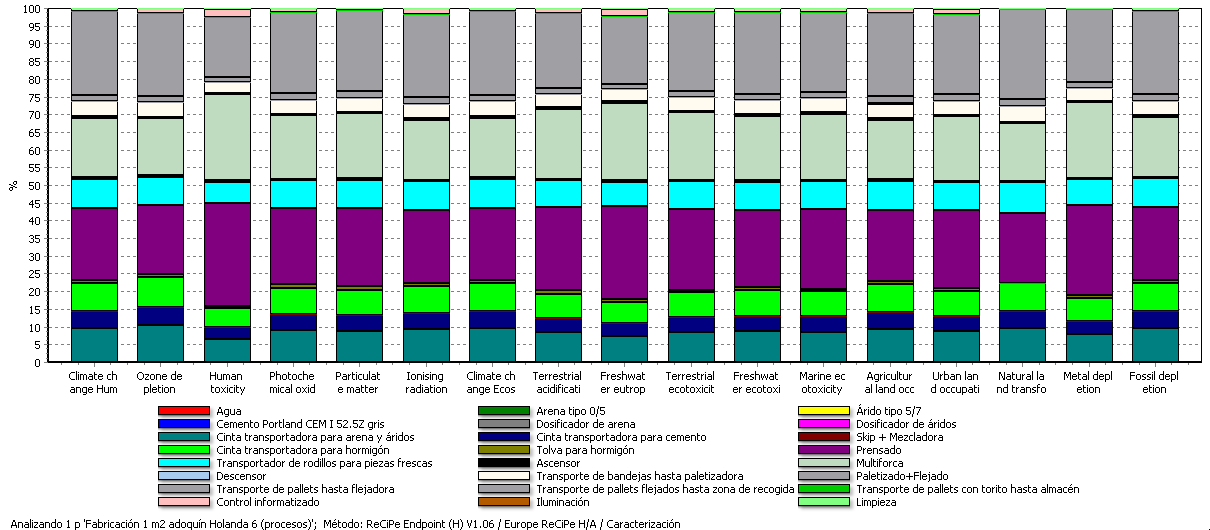
\includegraphics[angle=90,height=19cm]{fabricacion_caracterizacion.png}
\caption{Caracterización del análisis de fabricación de 1 \si{m^2} de adoquín.}
\label{fig:caracterizacionfabricacion}
\end{figure}

\begin{figure}[!htb]
\centering
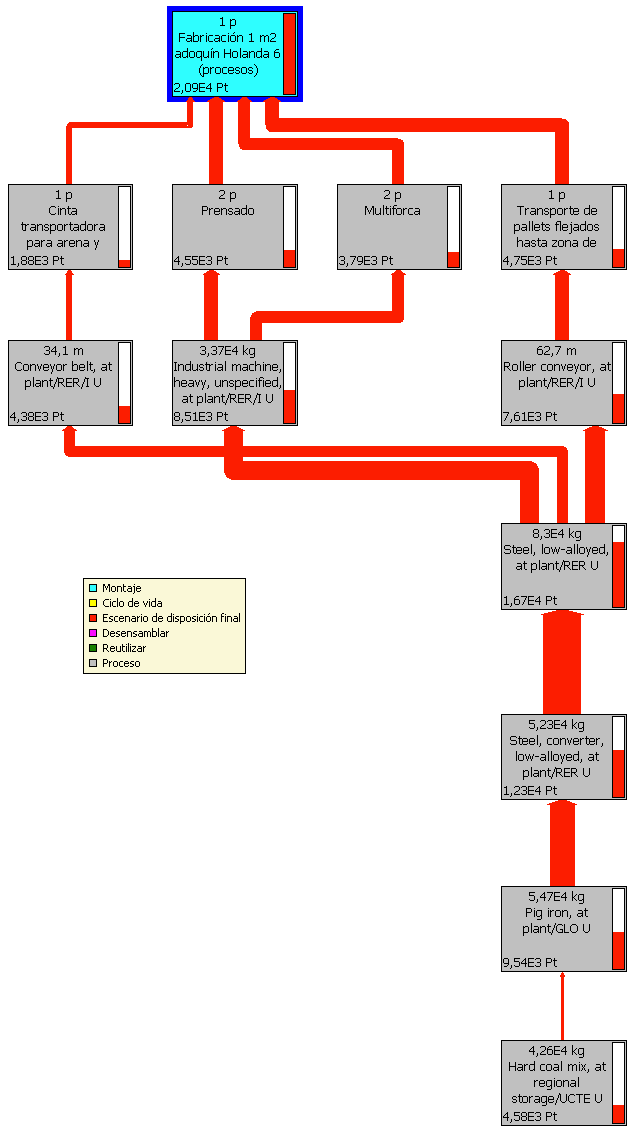
\includegraphics[height=19cm]{fabricacion_red.png}
\caption{Red del análisis de fabricación de 1 \si{m^2} de adoquín.}
\label{fig:redfabricacion}
\end{figure}

%!TEX root = informe.tex
\chapter{Análisis de Ciclo de Vida: instalación, uso y mantenimiento}
%(Fuente: Manual Técnico para la correcta colocación de los Euroadoquines (MTCE 04))
\section{Introducción}
La correcta colocación y mantenimiento del pavimento con adoquines es igual de importante que la calidad en los materiales y los procesos de fabricación \cite{euroadoquinc} para que el funcionamiento del pavimento sea el adecuado.

Hay múltiples manuales y guías técnicas que explican los criterios prácticos y recomendaciones para una correcta colocación de los adoquines.

La planificación del trabajo empieza estudiando el tipo de vía y uso principal al que estará destinado el pavimento. Una vez decidido es necesario preparar la explanada y las diferentes capas componentes en función de ese uso. A continuación se coloca la capa de adoquines, se sella con arena y se realiza un vibrado del pavimento. Por último se realiza una limpieza final.

\section{Capas componentes}

\begin{itemize}
\item Explanada: Terreno natural adecuadamente compactado hasta alcanzar una capacidad portante mínima.
\item Subbase: Conjunto de capas naturales, de material granular seleccionado, estabilizado y compactado, situadas directamente sobre la explanada.
\item Base: Principal elemento portante de la estructura, situada sobre la subbase. Puede ser realizada con material granular, zahorra artificial, con un mayor grado de compactación que el alcanzado en la subbase (Base Flexible), o estar realizada con hormigón magro (Base Rígida).
\item Lecho de árido: Base de apoyo de los adoquines, destinada a absorber sus diferencias de espesor debidas a la tolerancia de fabricación, de manera que estos una vez compactados formen una superficie homogénea.
\item Adoquines: Elementos prefabricados de hormigón, cuya cara exterior, una vez colocados, forman la capa de rodadura de la superficie a pavimentar.
\item Relleno final: Una vez encastrados en el lecho de árido, sus juntas precisan un relleno final para transferir a los elementos contiguos las cargas a las que sean sometidos por acción del tráfico.
\end{itemize}

\section{Determinación de la sección tipo}\label{sec:secciontipo}

Se consideran los siguientes casos:

\begin{enumerate}
\item Viales y zonas de aparcamiento\footnote{No suelen existir zonas peatonales puras (paso eventual de vehículos de mantenimiento, limpieza y servicios).}.
\item Zonas industriales.
\end{enumerate}


Para cada caso, viales o zonas industriales, la sección puede obtenerse de forma abreviada en función de dos variables:
\begin{itemize}
\item Tipo de explanadas.
\item Categoría de tráfico.
\end{itemize}

\subsection{Tipo de explanada}

Se utiliza un sistema de clasificación de su capacidad portante mediante el índice CBR (California Bearing Ratio), indicando el tanto por ciento de la presión ejercida por un pistón sobre el suelo para alcanzar una determinada penetración baremado según un juego de muestras normalizados (ver tabla \ref{indicecbr}.

\begin{table}[!htb]
\centering
\begin{tabular}{cc}
\toprule
Calidad de la explanada & Índice CBR\\
\midrule
E1 & 5 $\leq$ CBR = 10\\
E2 & 10 $\leq$ CBR = 20\\
E3 & 20 $\leq$ CBR\\
\bottomrule
\end{tabular}
\caption{Índice CBR.}
\label{indicecbr}
\end{table}


\subsection{Categoría de tráfico}

\begin{table}[!htb]
\centering
\begin{tabular}{cc}
\toprule
Tipo & Categoría de tráfico\\
\midrule
Viales y zonas de aparcamiento & C0 \ldots C4\\
Zonas industriales & A \ldots D\\
\bottomrule
\end{tabular}
\caption{Categoría de tráfico.}
\label{categoriadetrafico}
\end{table}

\subsubsection{Categorías de tráfico en viales y zonas de aparcamiento}

Si en un área limitada existen diversos usos, a efectos de unificación se debería emplear para toda la zona la carga de cálculo más exigente.

\begin{table}[!htb]
\centering
\begin{tabular}{p{7cm}c}
\toprule
Uso previsto & Categoría de tráfico\\
\midrule
Arterias principales con gran afluencia de tráfico, paradas de bus, estaciones de servicio, etc. (50 a 149 v.p.d.) & C0\\
Arterias principales (25 a 49 v.p.d.) & C1\\
Calles comerciales con gran actividad (16 a 24 v.p.d.) & C2\\
Calles comerciales cone escasa actividad (15 v.p.d.) & C3\\
Áreas peatonales, calles residenciales & C4\\
\bottomrule
\end{tabular}
\caption{Categoría de tráfico en viales y zonas de aparcamiento.}
\label{categoriadetraficoenviales}
\end{table}


\subsubsection{Categorías de tráfico en zonas industriales}

\begin{table}[!htb]
\centering
\begin{tabular}{cccc}
\toprule
\multicolumn{2}{c}{Área} & Uso & Intensidad de uso\\
\midrule
\multirow{7}{*}{Comercial} & De operación & — & Alta\\
& \multirow{2}{*}{Almacenamiento} & Mercancia convencional & Media\\
& & Mercancía pesada & Alta\\
& Manipulación & — & Alta\\
& \multirow{3}{*}{Estacionamiento} & Vehículos pesados y ligeros & Media\\
& & Vehículos pesados exclusivamente & Alta\\
& & Semirremolques & Alta\\
\midrule
\multirow{3}{*}{Militar} & De operación & — & Alta\\
& \multirow{2}{*}{Almacenamiento} & Mercancia convencional & Media\\
& & Mercancía pesada y semirremolques & Alta\\
\midrule
\multirow{3}{*}{Pesquera} & Almacenamiento & — & Media\\
& Manipulación & — & Alta\\
& Clasificación y venta & — & Media\\
\midrule
\multirow{3}{*}{Industrial} & De operación & — & Alta\\
& \multirow{2}{*}{Almacenamiento} & Mercancia convencional & Media\\
& & Mercancía pesada & Alta\\
\bottomrule
\end{tabular}
\caption{Intensidades de uso en zonas industriales.}
\label{categoriadetraficoenzonasindustrialesintensidades}
\end{table}


\begin{table}[!htb]
\centering
\begin{tabular}{cccc}
\toprule
Intensidad de uso & \multicolumn{3}{c}{Carga de cálculo}\\
\cmidrule{2-4}
& Alta & Media & Baja\\
\midrule
Elevada & A & B & C\\
Media & A & B & D\\
Reducida & B & C & D\\
\bottomrule
\end{tabular}
\caption{Categoría de tráfico en zonas industriales.}
\label{categoriadetraficoenzonasindustriales}
\end{table}

\section{Secciones tipo}

Las secciones tipo según la base y el uso previsto del área vistas en la sección \ref{sec:secciontipo} pueden resumirse en cinco tipos para cada tipo de base, granular (figura \ref{fig:seccionestipogranular}) u hormigón magro (figura \ref{fig:seccionestipohormigon}).

\begin{figure}[!htb]
\centering
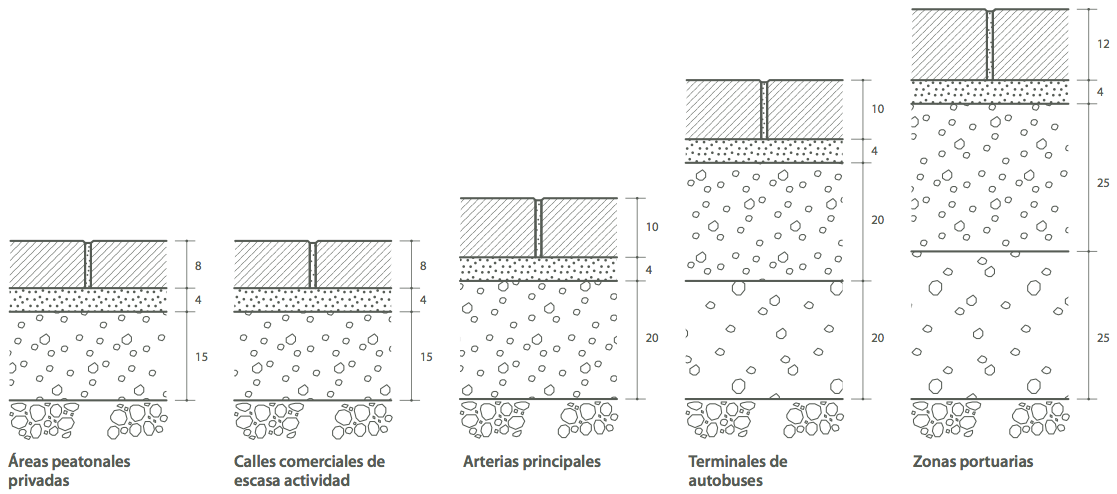
\includegraphics[width=15cm]{seccionestipo_1.png}
\caption[Secciones tipo para base granular.]{Secciones tipo para base granular. Unidades en cm. Fuente: \cite{fenollar}.}
\label{fig:seccionestipogranular}
\end{figure}

\begin{figure}[!htb]
\centering
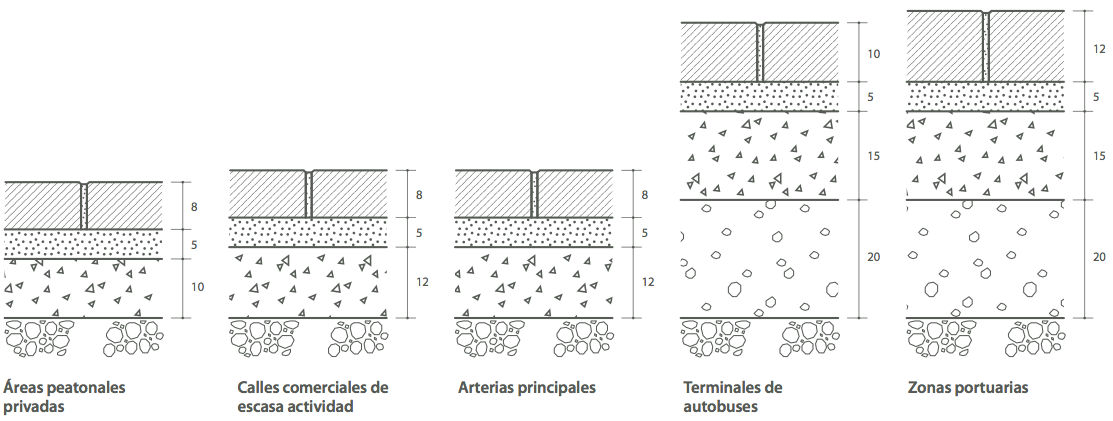
\includegraphics[width=15cm]{seccionestipo_2.png}
\caption[Secciones tipo para base de hormigón.]{Secciones tipo para base de hormigón. Unidades en cm. Fuente: \cite{fenollar}.}
\label{fig:seccionestipohormigon}
\end{figure}

\section{Modelado de los procesos}\label{sec:modeladoprocesosinstalacion}

Debido a que hay múltiples tipos de vía y uso destinado, se ha optado para el presente proyecto modelar la instalación más común, \textit{arterias principales}, que pertenece a la \textit{categoría de tráfico C1} y una \textit{calidad de explanada E2} con una base granular. Con esta clasificación, siguiendo las recomendaciones de \cite{euroadoquinc} el corte del terreno 1 \si{m^2} de superficie de terreno, que es la Unidad Funcional, será el reflejado en la tabla \ref{cortedelterreno}.

\begin{table}[!htb]
\centering
\begin{tabular}{lrrr}
\toprule
\multicolumn{4}{c}{Capas componentes para arterías principales C1-E2 con base granular}\\
\midrule
Capa componente & Grosor (\si{cm}) & Densidad (\si{kg/m^3}) & Volumen (\si{m^3})\\
\midrule
Adoquín \& Sellado & 10 & 2650 & 0.1\\
Lecho de árido & 4 & 1650 & 0.04\\
Base granular & 20 & 2560 & 0.2\\
Subbase & — & — & —\\
Explanada & \multicolumn{3}{c}{Aplanar y compactar}\\
\midrule
Total & 34 & — & 0.34\\
\bottomrule
\end{tabular}
\caption{Capas componentes para arterías principales C1-E2 con base granular.}
\label{cortedelterreno}
\end{table}

\subsection{Árido grueso para base granular (zahorra)}

Para la base granular es recomendable utilizar áridos calizos, y evitar en cualquier caso el uso de áridos con contenido en arcilla —arena de miga, arcillas refractarias—.

El acabado de la base debe ser similar al exigido para una superficie destinada a carreteras, usando una imprimación bituminosa. Tras compactar la base es recomendable hacer un sellado por medio de betún de curado rápido o emulsiones bituminosas para poder evitar filtraciones de agua a través de las juntas y que éstas dañen la base durante los primeros meses de la instalación.

La arena caliza —\textit{Limestone}, en inglés— aparece en la base de datos de SimaPro. Se pide como parámetro la masa de arena que se empleará para el rellenado. Si se tiene en cuenta que la base tiene una profundidad de 20 \si{cm} y un área de 1 \si{m^2}:

\begin{gather}
\text{Volumen de arena} = 0.2 \times 1 = 0.2 m^3\\
\rho_{arena}=2560 kg/m^3\\
\text{Masa de arena} = 0.2 \times 2560 = 512 kg
\end{gather}

Por otro lado, si se supone una distancia de entrega de 50 km hasta el destino de la instalación en un camión de transporte, se tiene:

\begin{equation}
512 kg \times 50 km = 25600 kg \times km
\end{equation}

\begin{table}[!htb]
\centering
\begin{tabular}{p{8cm}rc}
\toprule
\multicolumn{3}{c}{Arena para base granular}\\
\midrule
Materiales/ensamblajes & Cantidad & Unidad\\
\midrule
Limestone, milled, packed, at plant/CH U & 512 & \si{kg}\\
\midrule
Procesos & Cantidad & Unidad\\
\midrule
Transport, lorry 16-32t, EURO4/RER U & 25600 & \si{kg\times km}\\
\bottomrule
\end{tabular}
\caption{Modelado de la arena para base granular.}
\label{modeladoarenabase}
\end{table}

Igualmente, para la capa bituminosa de 5 cm que se aplica:

\begin{gather}
\text{Volumen de betún} = 0.05 \times 1 = 0.05 m^3\\
\rho_{betún}=1100 kg/m^3\\
\text{Masa de betún} = 0.05 \times 1100 = 55 kg
\end{gather}

Si se supone que el material proviene de una distancia de entrega de 50 km hasta el destino de la instalación en un camión de transporte, se tiene:

\begin{equation}
55 kg \times 50 km = 2750 kg \times km
\end{equation}

\begin{table}[!htb]
\centering
\begin{tabular}{p{8cm}rc}
\toprule
\multicolumn{3}{c}{Capa bituminosa para base granular}\\
\midrule
Materiales/ensamblajes & Cantidad & Unidad\\
\midrule
Bitumen sealing, at plant/RER U & 55 & \si{kg}\\
\midrule
Procesos & Cantidad & Unidad\\
\midrule
Transport, lorry 16-32t, EURO4/RER U & 2750 & \si{kg\times km}\\
\bottomrule
\end{tabular}
\caption{Modelado de la capa bituminosa para base granular.}
\label{modeladocapabituminosa}
\end{table}

\subsection{Árido semi-fino para lecho de arena}

La capa para el lecho de arena debe estar formada por áridos de resistencia geomecánica elevada, preferentemente de machaqueo ya que presentan mayores ángulos que mejoran la cohesión de la capa.

En general, los áridos deben ser poco finos, limpios y libres de elementos contaminantes.

La arena caliza —\textit{Limestone}, en inglés— aparece en la base de datos de SimaPro. Se pide como parámetro la masa de arena que se empleará para el rellenado. Si se tiene en cuenta que la base tiene una profundidad de 20 \si{cm} y un área de 1 \si{m^2}:

Sand, at mine/CH U 66
1650 kgm3
Transport 66*50

\begin{gather}
\text{Volumen de árido} = 0.04 \times 1 = 0.04 m^3\\
\rho_{arena}=1650 kg/m^3\\
\text{Masa de árido} = 0.04 \times 1650 = 66 kg
\end{gather}

Por otro lado, si se supone una distancia de entrega de 50 km hasta el destino de la instalación en un camión de transporte, se tiene:

\begin{equation}
66 kg \times 50 km = 3300 kg \times km
\end{equation}

\begin{table}[!htb]
\centering
\begin{tabular}{p{8cm}rc}
\toprule
\multicolumn{3}{c}{Árido semi-fino para lecho de arena}\\
\midrule
Materiales/ensamblajes & Cantidad & Unidad\\
\midrule
Gravel, crushed, at mine/CH U & 66 & \si{kg}\\
\midrule
Procesos & Cantidad & Unidad\\
\midrule
Transport, lorry 16-32t, EURO4/RER U & 3300 & \si{kg\times km}\\
\bottomrule
\end{tabular}
\caption{Modelado del árido semi-fino para lecho de arena.}
\label{modeladoaridosemifino}
\end{table}

\subsection{Arena para sellado}

La arena para sellado debe ser una arena sin exceso de finos, ya que si existen demasiados finos, se producirá un vaciado de las juntas con el uso y limpieza del pavimento o bien se filtrarás hacia el lecho.

Además debe ser libre de sales solubles y otros contaminantes, ya que pueden provocar la aparición de eflorescencias —igual que en el caso del lecho de árido—.

No se debe usar mortero para el sellado de las juntas, ya que no se podrán retirar para hacer tareas de mantenimiento —principal ventaja de los adoquines de hormigón—, además de perder flexibilidad del conjunto.

La arena de sílice —\textit{Silica sand}, en inglés— es un material adecuado para esta tarea \cite{website:cement}. SimaPro pide como parámetro la masa de arena que se empleará para el rellenado. Si se tiene en cuenta que el adoquín mide 10 \si{cm} de altura, 1 \si{cm} quedará enterrado en el lecho, y se añadirá 1 \si{cm} por encima para el vibrado; por otro lado, la junta medirá 5 \si{mm}, se puede obtener el volumen y a partir de él la masa:

\begin{gather}
1 m^2 = 50 \text{ adoquines} = 10 \times 5\\
Adoquin = 20 \times 10 \times 6 cm\\
\delta_{junta} = 0.5cm\\
Largo = 10 \times 10 + 9 \times 0.5 = 104.5 cm\\
Ancho = 5 \times 20 + 4 \times 0.5 = 102 cm\\
\text{Superficie de arena} = 104.5 \times 0.5 + 102 \times 0.5 = 103.25 cm^2\\
\text{Volumen de arena} = 103.25 \times 10 = 1032.5 cm^3\\
\rho_{arena}=2.6 g/cm^3\\
\text{Masa de arena} = 1032.5 \times 2.65 = 2.74 kg
\end{gather}

Por otro lado, si se supone una distancia de entrega de 50 km hasta el destino de la instalación en un camión de transporte, se tiene:

\begin{equation}
2.74 kg \times 50 km = 137 kg \times km
\end{equation}

\begin{table}[!htb]
\centering
\begin{tabular}{p{8cm}rc}
\toprule
\multicolumn{3}{c}{Arena para sellado}\\
\midrule
Materiales/ensamblajes & Cantidad & Unidad\\
\midrule
Silica sand, at plant/DE U & 2.74 & \si{kg}\\
\midrule
Procesos & Cantidad & Unidad\\
\midrule
Transport, lorry 16-32t, EURO4/RER U & 137 & \si{kg\times km}\\
\bottomrule
\end{tabular}
\caption{Modelado de la arena para sellado.}
\label{modeladoarenasellado}
\end{table}

\subsection{Excavación del terreno}

A la hora de realizar un pavimento de adoquines, se debe realizar en primer lugar la excavación del terreno. Dado que el grosor total de las capas componentes es de 34 \si{cm} y se dispone de un área de 1 \si{m^2}, el volumen a introducir para el modelo será 0.34 \si{m^3}, utilizando como entrada de SimaPro de excavación con herramienta hidráulica, \textit{Excavation, hydraulic digger}.

\begin{table}[!htb]
\centering
\begin{tabular}{p{8cm}rc}
\toprule
\multicolumn{3}{c}{Excavación del terreno}\\
\midrule
Materiales/combustibles & Cantidad & Unidad\\
\midrule
Excavation, hydraulic digger/RER U & 0.34 & \si{m^3}\\
\bottomrule
\end{tabular}
\caption{Modelado de la excavación del terreno.}
\label{modeladoexcavacion}
\end{table}

\subsection{Compactación de la explanada}

Una vez excavado el terreno es necesario compactar lo que será la explanada. La bibliografía consultada no ha ofrecido ninguna solución óptima a este tipo de proceso, por lo que se ha optado por asemejar el tipo de trabajo de un tractor usando un rodillo para cultivar la tierra —\textit{Tillage, rolling}, en inglés— con el rodillo utilizado por una apisonadora o compactadora —\textit{road roller}, en inglés—. En este caso, la compactación se realiza en unidades de área, por lo que se ha introducido 1 \si{m^2} de superficie.

\begin{table}[!htb]
\centering
\begin{tabular}{p{8cm}rc}
\toprule
\multicolumn{3}{c}{Compactación de la explanada}\\
\midrule
Materiales/combustibles & Cantidad & Unidad\\
\midrule
Tillage, rolling/CH U & 1 & \si{m^2}\\
\bottomrule
\end{tabular}
\caption{Modelado de la compactación de la explanada.}
\label{modeladoexplanada}
\end{table}

\subsection{Compactación de la capa base}

En el caso de arterias principales no existe una capa subbase, por lo que se procederá a la extensión y compactación de la capa base. Una correcta ejecución es fundamental ya que esta capa es el principal elemento portante de la estructura y se encarga de transmitir hacia la explanada las cargas verticales. El espesor de esta base debe ser uniforme.

Es muy importante que el plano de la capa base respete una pendiente mínima del 1\% para permitir un drenaje adecuado de las aguas superficiales sin que provoquen daños a las capas portantes, y así evitar daños en la superficie.

La bibliografía consultada no ha ofrecido ninguna solución óptima a este tipo de proceso, por lo que se ha optado por asemejar el tipo de trabajo de un tractor usando un rodillo para cultivar la tierra —\textit{Tillage, rolling}, en inglés— con el rodillo utilizado por una apisonadora o compactadora —\textit{road roller}, en inglés—. En este caso, la compactación se realiza en unidades de área, por lo que se ha introducido 1 \si{m^2} de superficie.

\begin{table}[!htb]
\centering
\begin{tabular}{p{8cm}rc}
\toprule
\multicolumn{3}{c}{Compactación de la capa base}\\
\midrule
Materiales/combustibles & Cantidad & Unidad\\
\midrule
Tillage, rolling/CH U & 1 & \si{m^2}\\
\bottomrule
\end{tabular}
\caption{Modelado de la compactación de la capa base.}
\label{modeladocapabase}
\end{table}

\subsection{Compactación del lecho de árido}

El lecho de árido es, junto con la calidad del adoquín, el elemento fundamental que determina el comportamiento y durabilidad del pavimento. El lecho se extiende directamente sobre la capa base.

Una de las funciones principales es la de absorber las pequeñas diferencias de espesor de los adoquines siguiendo las tolerancias de la normativa \cite{une1338}, de forma que, una vez se hace la compactación de los adoquines, formen un plano de rodadura uniforme que transmita las cargas del tráfico sin deteriorar las piezas.

Otra de las funciones del lecho de árido es la de actuar como elemento de relleno inferior de las juntas de los adoquines. Al ser compactados los adoquines, quedan incrustados en el lecho, y así se evita el contacto directo entre las caras laterales de las piezas.


Al igual que en las compactaciones anteriores, la bibliografía consultada no ha ofrecido ninguna solución óptima a este tipo de proceso, por lo que se ha optado por asemejar el tipo de trabajo de un tractor usando un rodillo para cultivar la tierra —\textit{Tillage, rolling}, en inglés— con el rodillo utilizado por una apisonadora o compactadora —\textit{road roller}, en inglés—. En este caso, la compactación se realiza en unidades de área, por lo que se ha introducido 1 \si{m^2} de superficie.

\begin{table}[!htb]
\centering
\begin{tabular}{p{8cm}rc}
\toprule
\multicolumn{3}{c}{Compactación del lecho de árido}\\
\midrule
Materiales/combustibles & Cantidad & Unidad\\
\midrule
Tillage, rolling/CH U & 1 & \si{m^2}\\
\bottomrule
\end{tabular}
\caption{Modelado de la compactación del lecho de árido.}
\label{modeladolecho}
\end{table}

\subsection{Sellado con arena y vibrado del pavimento}

Una vez colocados y alineados los adoquines de forma que el lecho de árido también sirva de separador entre las juntas, se extiende sobre el pavimento una capa ligera de arena para completar el espacio.

La importancia de esta etapa yace en que un relleno completo de las juntas hace que tanto esta arena como el árido del leche sean los transmisores de los esfuerzos laterales entre los adoquines. Si el pavimento soporta tráfico sin haber sido bien sellado, se pueden producr daños importantes sobre el mismo.

El sellado consiste en extender arena fina y seca sobre el pavimento e introducirla entre las juntas con un barrido manual o mecánico, intentando que quede una ligera capa de excedente sobre toda la superficie.

A continuación se realiza un proceso de compactación sobre el pavimento para garantizar un relleno adecuado de las juntas. Esta compactación se puede realizar bien con placas vibrantes —\textit{vibratory plates} o \textit{plate compactor}, en inglés— o con rodillos mecánicos con vibración. La fuerza vibratoria y el peso de las herramientas deben ser proporcionales al tipo de pavimento que se está ejecutando.

Una vez se realiza la compactación, el pavimento puede ponerse en servicio inmediatamente.

El proceso de compactación no aparece reflejado en las librerías que proporciona SimaPro. De acuerdo a \cite{rieradevall}, las placas vibrantes para compactar pueden modelarse mediante su consumo de combustible. En concreto 2.43 \si{MJ} de gasoil para 1 ft$^2$. Por lo que, extrapolando para 1 \si{m^2}, se tendría:

\begin{equation}
2.43\frac{MJ}{{ft}^2} \times \frac{10.764{ft^2}}{1m^2}=26.16MJ/m^2
\end{equation}

\begin{table}[!htb]
\centering
\begin{tabular}{p{8cm}rc}
\toprule
\multicolumn{3}{c}{Vibrado del pavimento}\\
\midrule
Materiales/combustibles & Cantidad & Unidad\\
\midrule
Diesel, burned in building machine/GLO U & 26.16 & \si{MJ}\\
\bottomrule
\end{tabular}
\caption{Modelado del vibrado del pavimento.}
\label{modeladovibrado}
\end{table}

\subsection{Limpieza final}

Cuando se ha terminado el vibrado del pavimento y se ha observado que las juntas quedan completamente rellenas, se debe iniicar el proceso de limpieza de la superficie para eliminar la arena de sellado excedente.

Esta limpieza se realiza mediante un barrido manual, dejando una pequeña capa de arena sobre el pavimento para que el tráfico termine de colocar sobre las juntas de forma natural. Una vez finalizada la limpieza se puede abrir la vía al uso destinado.

Este proceso no se ha incluido en SimaPro ya que es un trabajo manual de un operario y no se consumen directamente materiales o combustibles.

\section{Modelado completo}

Los modelos de los procesos explicados en la sección \ref{sec:modeladoprocesosinstalacion} han sido introducidos en SimaPro para crear un modelo completo que represente la instalación de un metro cuadrado de adoquín modelo Holanda 6. El listado completo de procesos se muestra en la tabla \ref{modeladocompletoinstalacion}.

\begin{table}[!htb]
\centering
\begin{tabular}{p{8cm}rc}
\toprule
\multicolumn{3}{c}{Fabricación 1 \si{m^2} adoquín Holanda 6}\\
\midrule
Materiales/ensamblajes & Cantidad & Unidad\\
\midrule
Árido grueso para base granular (zahorra) & 1 & p\\
Capa bituminosa para base granular (zahorra) & 1 & p\\
Árido semi-fino para lecho de arena & 1 & p\\
Arena para sellado de juntas & 1 & p\\
\midrule
Procesos & Cantidad & Unidad\\
\midrule
Excavación del terreno para arteria principal C1-E2 & 1 & p\\
Compactación de la explanada & 1 & p\\
Compactación de la capa base & 1 & p\\
Compactación del lecho de arena & 1 & p\\
Sellado+vibrado del pavimento & 1 & p\\
\bottomrule
\end{tabular}
\caption{Modelado completo de la instalación.}
\label{modeladocompletoinstalacion}
\end{table}

\section{Resultados}

Una vez creado el modelo completo del proceso de instalación, SimaPro genera un análisis de los datos introducidos. El método de análisis elegido es \textit{ReCiPe Endpoint (H) V1.06 / Europe ReCipe H/A}, previamente explicado en la sección \ref{sec:recipe}.

\begin{figure}[!htb]
\centering
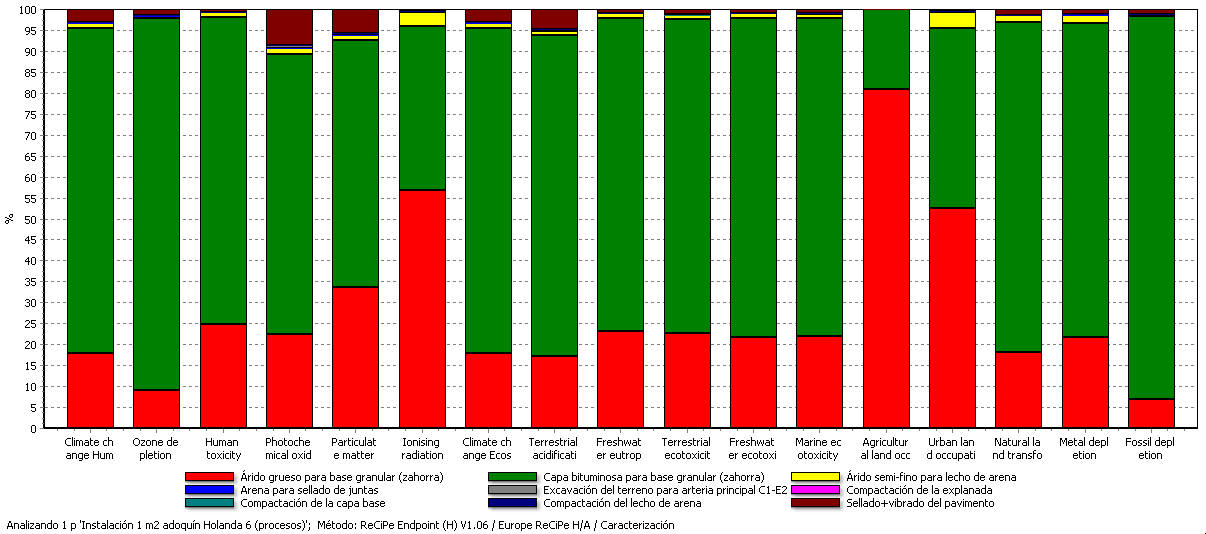
\includegraphics[angle=90,height=19cm]{instalacion_caracterizacion.png}
\caption{Caracterización del análisis de instalación de 1 \si{m^2} de adoquín.}
\label{fig:caracterizacioninstalacion}
\end{figure}

\begin{figure}[!htb]
\centering
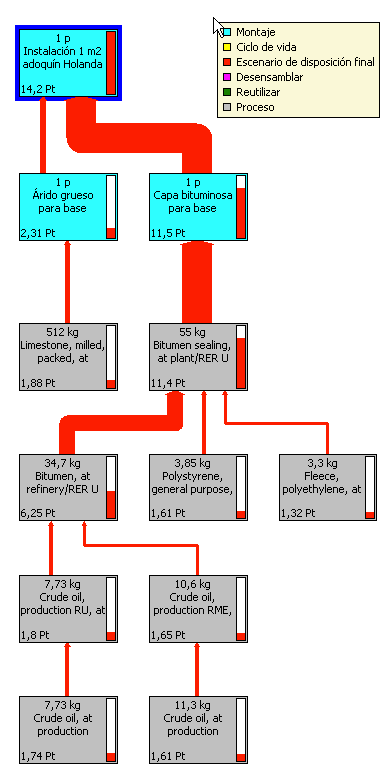
\includegraphics[height=19cm]{instalacion_red.png}
\caption{Red del análisis de instalación de 1 \si{m^2} de adoquín.}
\label{fig:redinstalacion}
\end{figure}

%!TEX root = informe.tex
\chapter{Análisis de Ciclo de Vida: uso y mantenimiento}

\section{Introducción}\label{sec:introduccionuso}

Una de las principales ventajas del pavimento con adoquines de hormigón es el fácil y económico mantenimiento del mismo durante su vida útil. Aunque la esperanza de vida de un adoquín está probada en 50 años, su tiempo de diseño es únicamente 30 años \cite{euroadoquin}.

Para que el funcionamiento del pavimento sea el correcto, las juntas deben permanecer llenas de arena —la presencia de pasto en las juntas no es nociva—. Si se pierde más de 1 \si{cm} de sello se debe corregir el hueco con arena de sellado.

Si se hunde el pavimento o es necesario acceder a infraestructura urbana, se deben retirar los adoquines, realizar la reparación y volver a reconstruir la franja de pavimento. La presencia de ondulaciones en la superficie del pavimento puede ser un indicio de que fue construido con una base mal construida o las características del tráfico no son las de diseño.

El pavimento de adoquines debe limpiarse, en principio, únicamente por barrido. El lavado con manguera debe ser poco frecuente y sólo cuando el tamaño de las juntas sea pequeño.

Existe un mantenimiento periódico, cada 3—5 años, que consiste en renovar el sellado del pavimento debido a la acción erosiva del medio ambiente \cite{malaka}.


\section{Modelado de materias primas y procesos}\label{sec:modeladoprocesosusoymantenimiento}

El pavimento de adoquines puede presentar tres situaciones durante su vida útil en las que intervengan recursos adicionales para su uso y mantenimiento:
\begin{itemize}
\item limpieza.
\item sellado de juntas.
\item apertura del pavimento por rotura o infraestructura urbana.
\end{itemize}

En los dos primeros casos se puede establecer un modelo debido a que existe un patrón periódico sobre el que diseñarlo. Sin embargo, el tercero no es posible establecer un modelo sencillo que prevea ese comportamiento, por lo que se procederá a idealizar el uso y mantenimiento del mismo sin roturas.

\subsection{Limpieza mensual}
Si se tiene en cuenta lo establecido en la sección \ref{sec:introduccionuso}, se riega el pavimento una vez al mes en el que se consumen 5 litros de agua por cada metro cuadrado de adoquín instalado.

\begin{table}[!htb]
\centering
\begin{tabular}{p{8cm}rc}
\toprule
\multicolumn{3}{c}{Limpieza mensual}\\
\midrule
Materiales/combustibles & Cantidad & Unidad\\
\midrule
Tap water, at user/RER/I U & 5 & \si{kg}\\
\bottomrule
\end{tabular}
\caption{Modelado la limpieza de mensual del pavimento.}
\label{modeladolimpiezamensual}
\end{table}

\subsection{Sellado de juntas}

Si se supone una labor de mantenimiento periódica cada 5 años de sellado de juntas, y la vida útil se considera de 30 años (sección \ref{sec:introduccionuso}), se realizarán 6 sellados de juntas en el transcurso de su vida.

Para el cálculo se puede utilizar lo expuesto en la sección \ref{sec:selladoinstalacion}, utilizando la misma arena —arena silícea— y procedimiento de instalación —vibrado del pavimento. En este caso, se supondrá que las pérdidas de arena no van a ser del 100\% sino del 50\% de la masa inicial de arena de sellado instalada, transportada en camión una distancia de 50 \si{km}.

\begin{table}[!htb]
\centering
\begin{tabular}{p{8cm}rc}
\toprule
\multicolumn{3}{c}{Arena para sellado para mantenimiento}\\
\midrule
Materiales/ensamblajes & Cantidad & Unidad\\
\midrule
Silica sand, at plant/DE U & 1.37 & \si{kg}\\
\midrule
Procesos & Cantidad & Unidad\\
\midrule
Transport, lorry 16-32t, EURO4/RER U & 68.5 & \si{kg\times km}\\
\bottomrule
\end{tabular}
\caption{Modelado de la arena para sellado para mantenimiento.}
\label{modeladoarenaselladomantenimiento}
\end{table}

\begin{table}[!htb]
\centering
\begin{tabular}{p{8cm}rc}
\toprule
\multicolumn{3}{c}{Vibrado del pavimento para uso y mantenimiento}\\
\midrule
Materiales/combustibles & Cantidad & Unidad\\
\midrule
Diesel, burned in building machine/GLO U & 26.16 & \si{MJ}\\
\bottomrule
\end{tabular}
\caption{Modelado del vibrado del pavimento para uso y mantenimiento.}
\label{modeladovibradouso}
\end{table}

\section{Modelado completo}

\section{Resultados}

%!TEX root = informe.tex
\chapter{Análisis de Ciclo de Vida: fin de vida}
Manual Euroadoquín2
\section{Introducción}
\section{Reciclaje}
\section{Procesos}

%!TEX root = informe.tex
\chapter{Conclusiones}\label{cap:conclusiones}
\section{Conclusiones generales}
En este proyecto se ha realizado un Análisis de Ciclo de Vida de un adoquín prefabricado de cemento de dimensiones 200\times 100\times 60 \si{mm}, tomando como unidad funcional un metro cuadrado del mismo.

El estudio de ACV supone una potente herramienta para detectar los procesos con mayor carga ambiental y los impactos ocasionados al medioambiente de forma normalizada y objetiva. Una vez se localizan estos puntos calientes pueden comunicarse a la empresa para realizar mejoras en el proceso repercutiendo bien energéticamente, económicamente o como publicidad de tipo ambiental. Se puede recurrir al etiquetado ambiental \cite{iso14020} para estimular la demanda de productos y servicios con menores cargas ambientales indicando información relevante sobre su ciclo de vida —tal como la energía consumida o la cantidad de \ce{CO2} generado— y así satisfacer una demanda creciente de productos con información ambiental.

La carga ambiental mayor se produce en la fase del ciclo de vida de extracción de materias primas, fabricación e instalación, siendo la fase de uso y mantenimiento muy inferior aunque no despreciable y la de fin de vida tomada en consideración por los beneficios ambientales que aporta.

Los procesos unitarios donde se producen las mayores cargas ambientales son la extracción de materias primas para la capa bituminosa y el árido grueso de la capa base de la instalación y el proceso de fabricación del cemento Portland.

La fase del Análisis de Ciclo de Vida más compleja es la de Inventario de Ciclo de Vida, debido a que el inventario que ofrece la base de datos \textit{ecoinvent} no disponía de la amplia mayoria de procesos que intervienen en este proyecto y la información disponible era muy reducida. También ha aportado complejidad a la realización de este proyecto la baja disponibilidad de otros proyectos que sirvieran de base que utilizaran el ACV como método de estudio en este sector.

El software de análisis SimaPro ha simplificado en gran medida la fase de Evaluación del Inventario de Ciclo de Vida y la de Interpretación, no sólo por la incorporación del método ReCiPe, sino por su adaptación del flujo de trabajo a la normativa UNE-EN-ISO 14040:2006 y 14044:2006.


\section{Futuros trabajos y ampliaciones}

Este método de análisis desarrollado durante este proyecto es aplicable no sólo a adoquines sino a cualquier producto o servicio, por lo que se puede usar como base para otros productos prefabricados del cemento u otros tipos de pavimentos como el de asfalto o cerámico para poder hacer comparaciones entre ellos.

También se podría ampliar el estudio a otros países —donde cambiaría el mix eléctrico— u otros procesos alternativos de fabricación distintos al de este estudio.

\cleardoublepage

\part{Anexos}
\begin{appendices}
%!TEX root = informe.tex
\chapter{Datos proporcionados por el fabricante}\label{apend:datos}
En este apéndice se incluyen los datos proporcionados por el fabricante acerca del proceso de producción.

\begin{table}[!htb]
\centering
\begin{tabular}{lccc}
\toprule
\multicolumn{4}{c}{Fórmula base para de adoquín Holanda 6}\\
\midrule
Materia prima & \% Fórmula & Proced. & Dist. (\si{km})\\
\midrule
Árido tipo 5/7 & 37.75 & Alh. Torre & 8\\
Arena tipo 0/5 & 47.16 & Alh. Torre & 8\\
Cemento Portland 52.5N & 10.06 & Málaga-El Palo & 30\\
Agua & 5.03 & Red & -\\
\bottomrule
\end{tabular}
\caption{Fórmula base para de adoquín Holanda 6.}
\label{formulabase}
\end{table}

\begin{figure}[!htb]
\centering
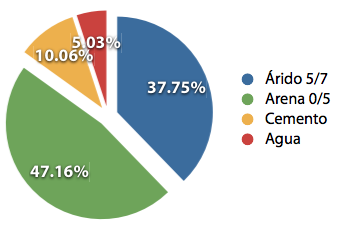
\includegraphics[width=6cm]{porcent_matprima.png}
\caption{Porcentajes de materías prima para adoquín.}
\label{fig:porcentmatprima}
\end{figure}

\begin{table}[!htp]
\centering
\begin{tabular}{lcrrr}
\toprule
\multicolumn{5}{c}{Tiempo de proceso y energía por \si{m^2} de adoquín fabricado}\\
\midrule
Proceso & Duración (\si{s}) & Pot. (\si{kW}) & Energía (\si{kJ}) & Energía (\si{MJ})\\
\midrule
Dosif. arena & 3 & 0.7 & 2.1 & 0.0021\\
Dosif. áridos & 3 & 0.7 & 2.1 & 0.0021\\
Cinta transp. arena y áridos  & 21 & 8.7 & 182.7 & 0.1827\\
Cinta transp. cemento & 15 & 6.5 & 97.5 & 0.0975\\
Skip  & 27 & 15 & 405 & 0.405\\
Mezcladora & 42 & 31 & 1302 & 1.302\\
Cinta transp. hormigón & 11 & 8 & 88 & 0.088\\
Tolva hormigón 1/2 & 23 & 0.7 & 16.1 & 0.0161\\
Prensado 1/2 & 19 & 23 & 437 & 0.437\\
Cinta transp. piezas frescas 1/2 & 14 & 5.5 & 77 & 0.077\\
Ascensor 1/2 & 1 & 7 & 7 & 0.007\\
Tolva hormigón 2/2 & 23 & 0.7 & 16.1 & 0.0161\\
Prensado 2/2 & 19 & 23 & 437 & 0.437\\
Cinta piezas frescas 2/2 & 14 & 5.5 & 77 & 0.077\\
Ascensor 2/2 & 17 & 7 & 119 & 0.119\\
Multiforca ida & 43 & 12 & 516 & 0.516\\
Multiforca vuelta & 43 & 12 & 516 & 0.516\\
Descensor 1/2 & 17 & 7 & 119 & 0.119\\
Descensor 2/2 & 1 & 7 & 7 & 0.007\\
Transp. bandejas hasta paletiz. & 14 & 1.5 & 21 & 0.021\\
Paletizadora & 10 & 5 & 50 & 0.05\\
Transp. palet & 14 & 1.7 & 23.8 & 0.0238\\
Flejadora & 10 & 1.5 & 15 & 0.015\\
Transp. rodillos hasta recogida  & 21 & 1.5 & 31.5 & 0.0315\\
Control informatizado & 405 & 1.2 & 486 & 0.486\\
Iluminación & 405 & 2.4 & 972 & 0.972\\
\bottomrule
\end{tabular}
\caption{Desglose de procesos y energías del fabricante por \si{m^2} de adoquín fabricado.}
\label{desgloseenergia}
\end{table}

\begin{figure}[!htb]
\centering
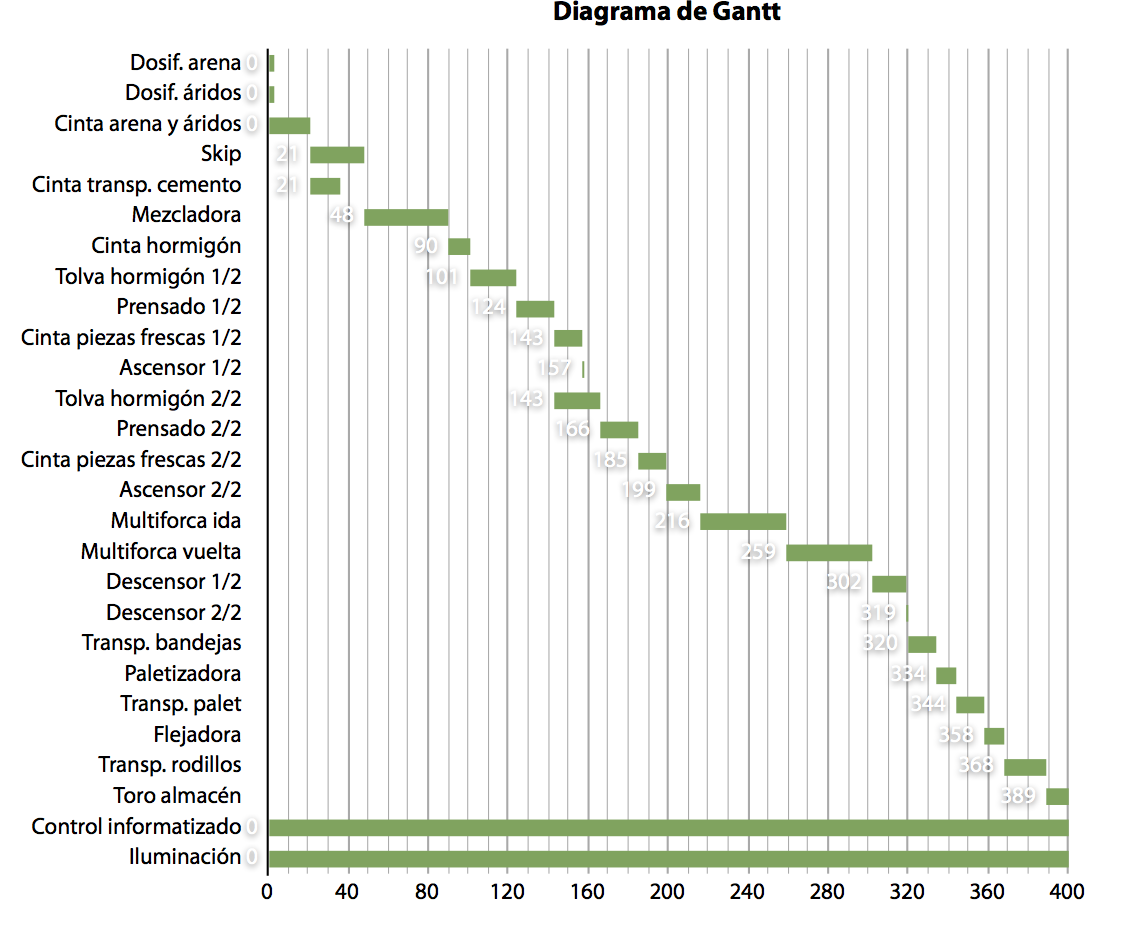
\includegraphics[width=15cm]{gantt.png}
\caption{Diagrama de Gantt de los procesos de fabricación.}
\label{fig:gant}
\end{figure}

\cleardoublepage
%!TEX root = informe.tex
\chapter{Resultados de SimaPro}\label{apend:simapro}
En este apéndice se incluyen los resultados de la aplicación de software SimaPro.

\cleardoublepage
%!TEX root = informe.tex
\chapter{Catálogo Adoquín Holanda 6}\label{apend:catalogo}
En este apéndice se incluyen los planos de la planta de fabricación de materiales prefabricados y los modelos de fabricación del adoquín y su molde.

\newpage
\begin{figure}[!htb]
\centering
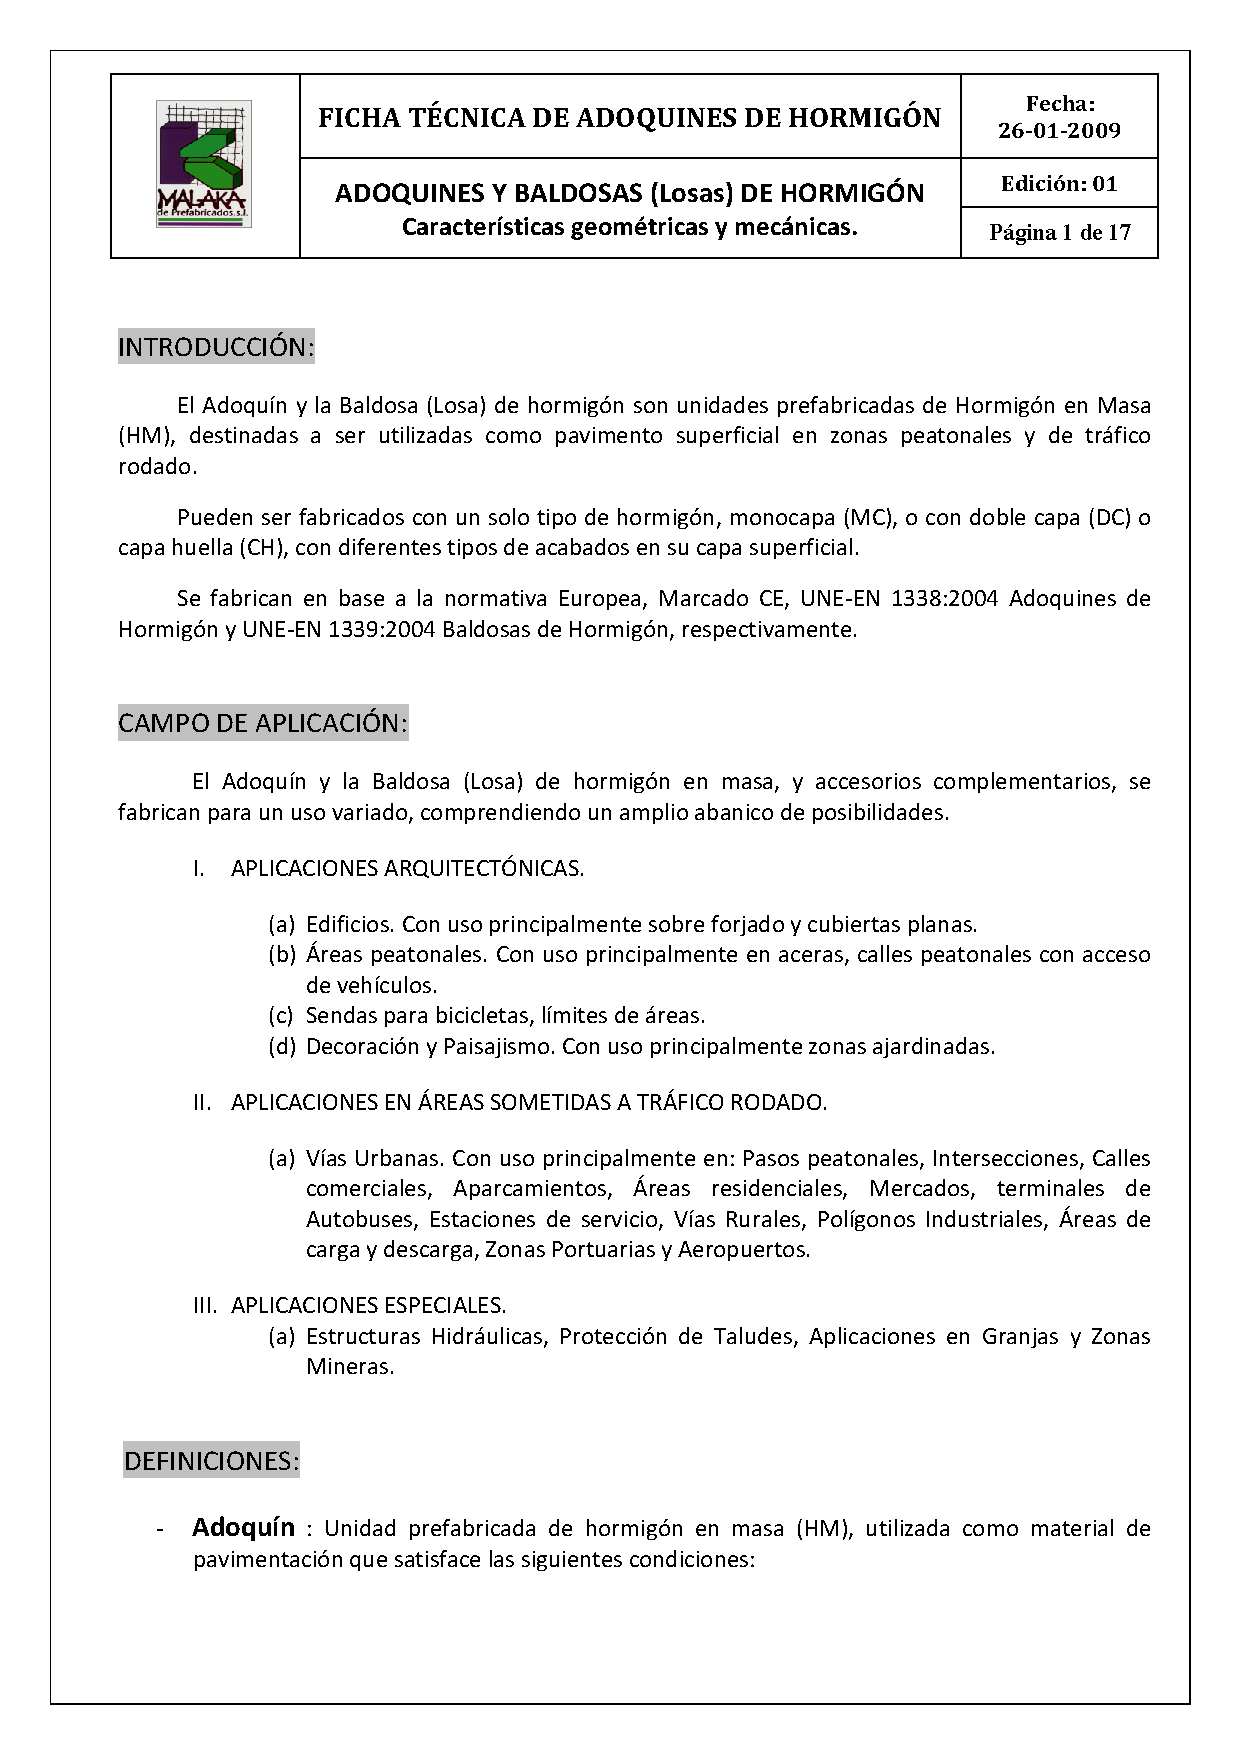
\includegraphics[scale=0.68]{ficha_tecnica/ft_adoquin_1.pdf}
\label{fig:ftadoquin1}
\end{figure}
\newpage
\begin{figure}[!htb]
\centering
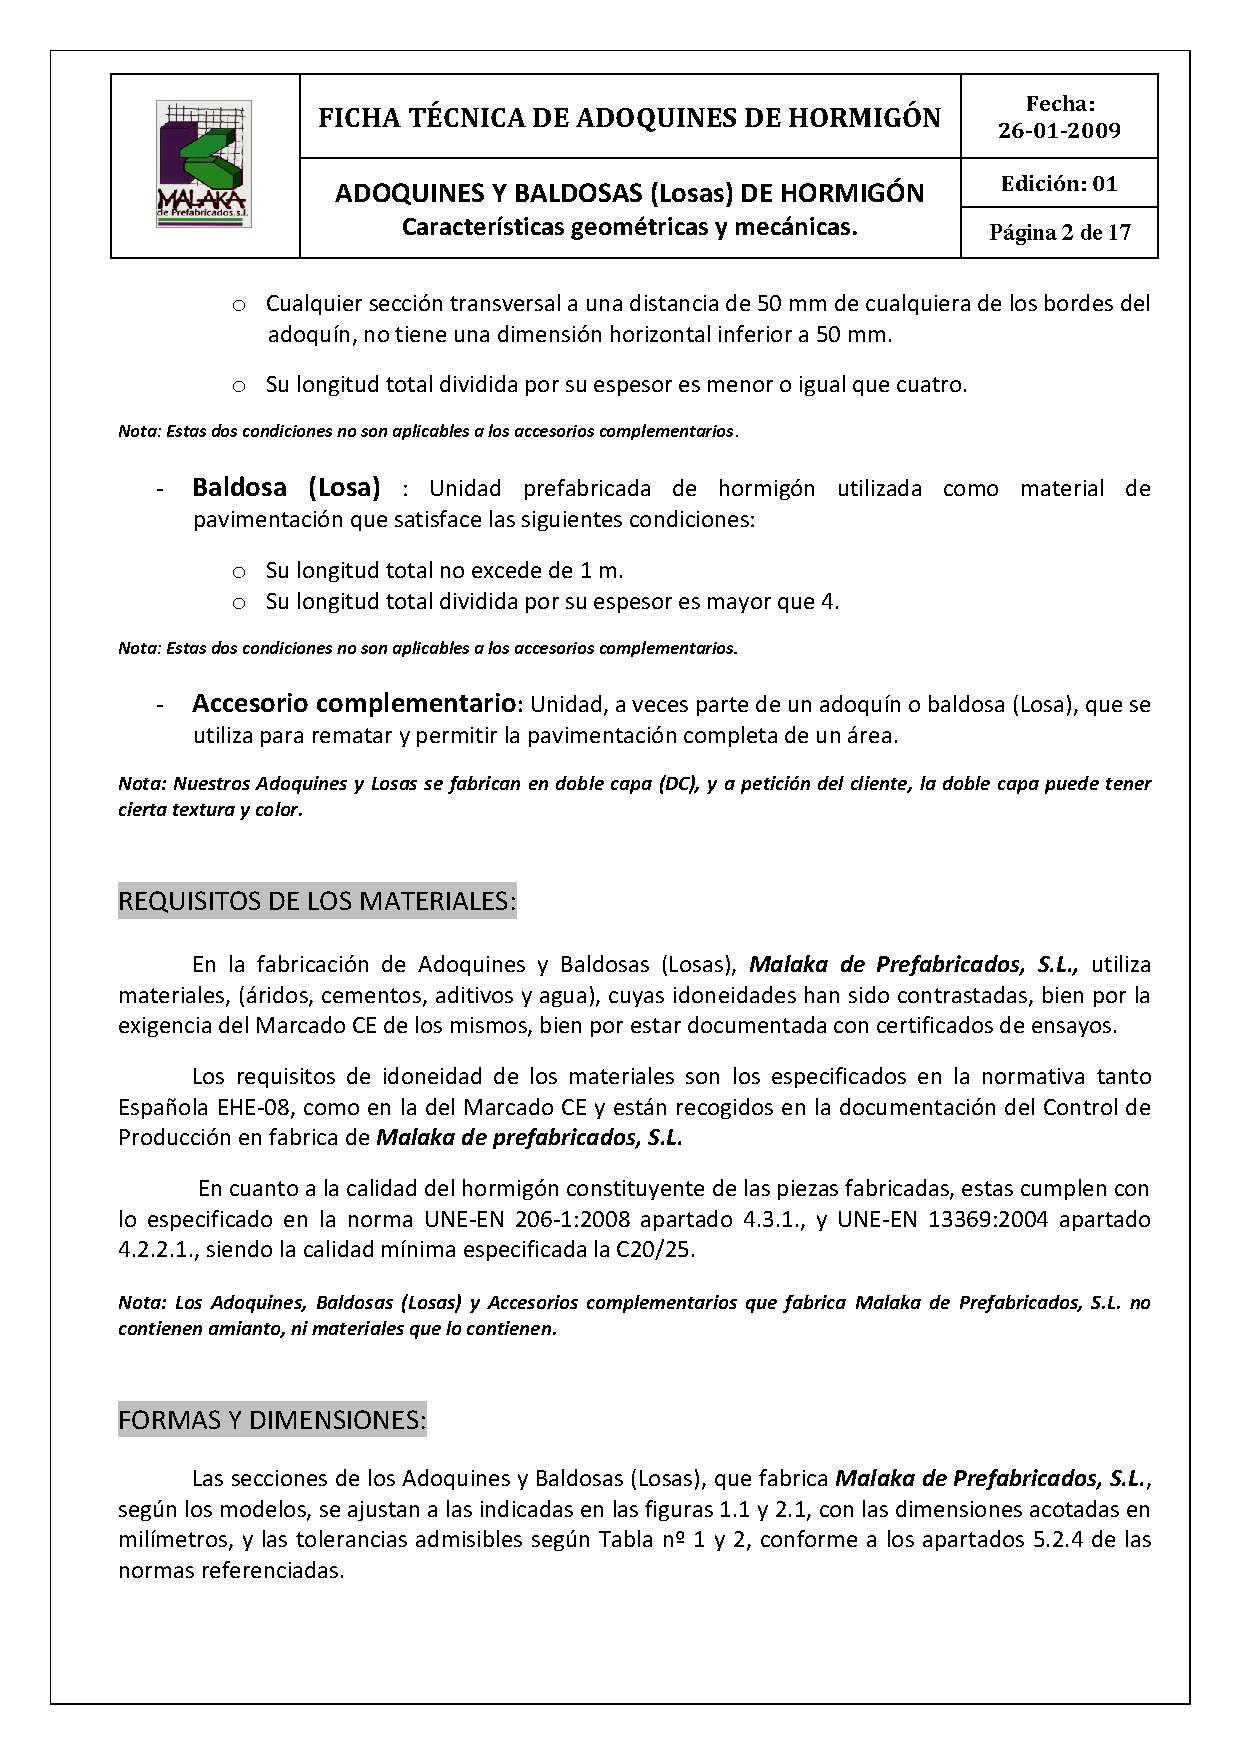
\includegraphics[scale=0.68]{ficha_tecnica/ft_adoquin_2.pdf}
\label{fig:ftadoquin2}
\end{figure}
\newpage
\begin{figure}[!htb]
\centering
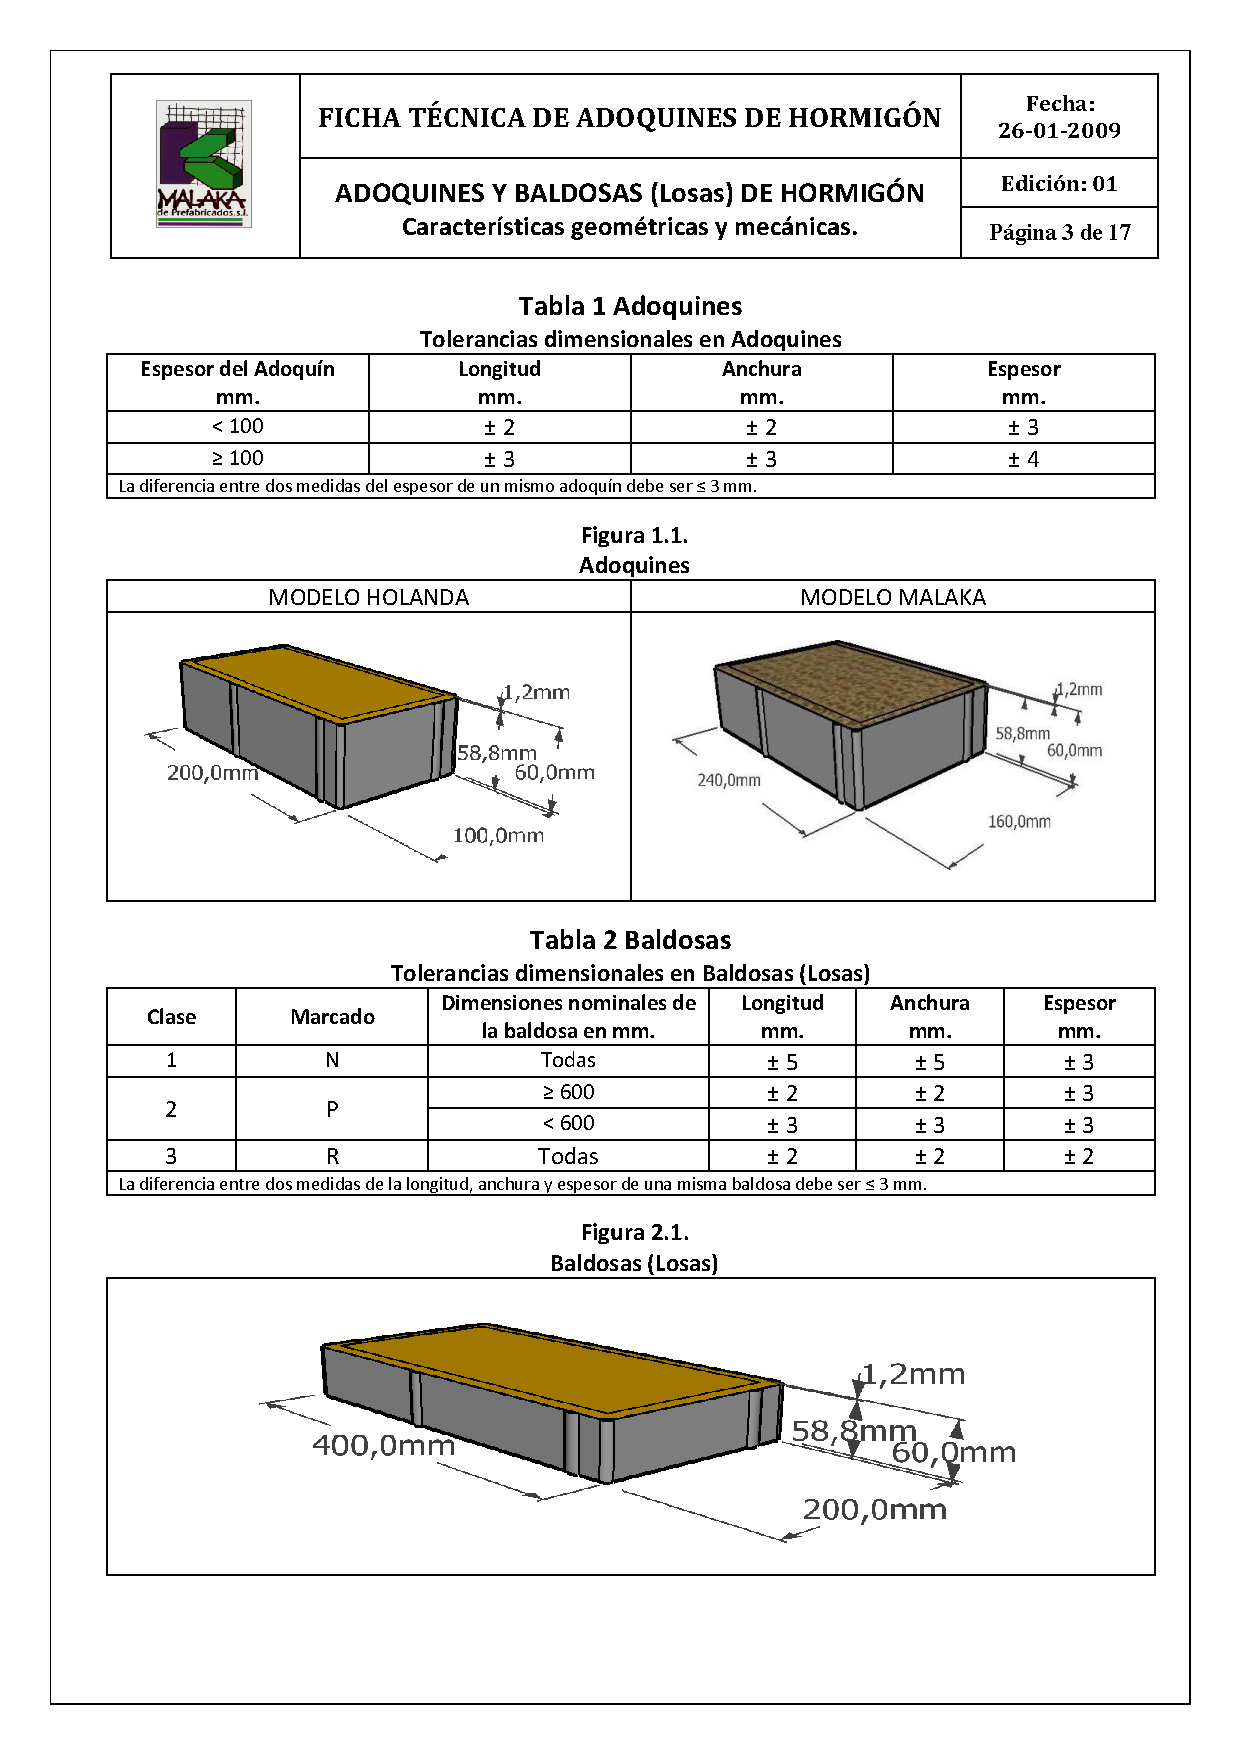
\includegraphics[scale=0.68]{ficha_tecnica/ft_adoquin_3.pdf}
\label{fig:ftadoquin3}
\end{figure}
\newpage
\begin{figure}[!htb]
\centering
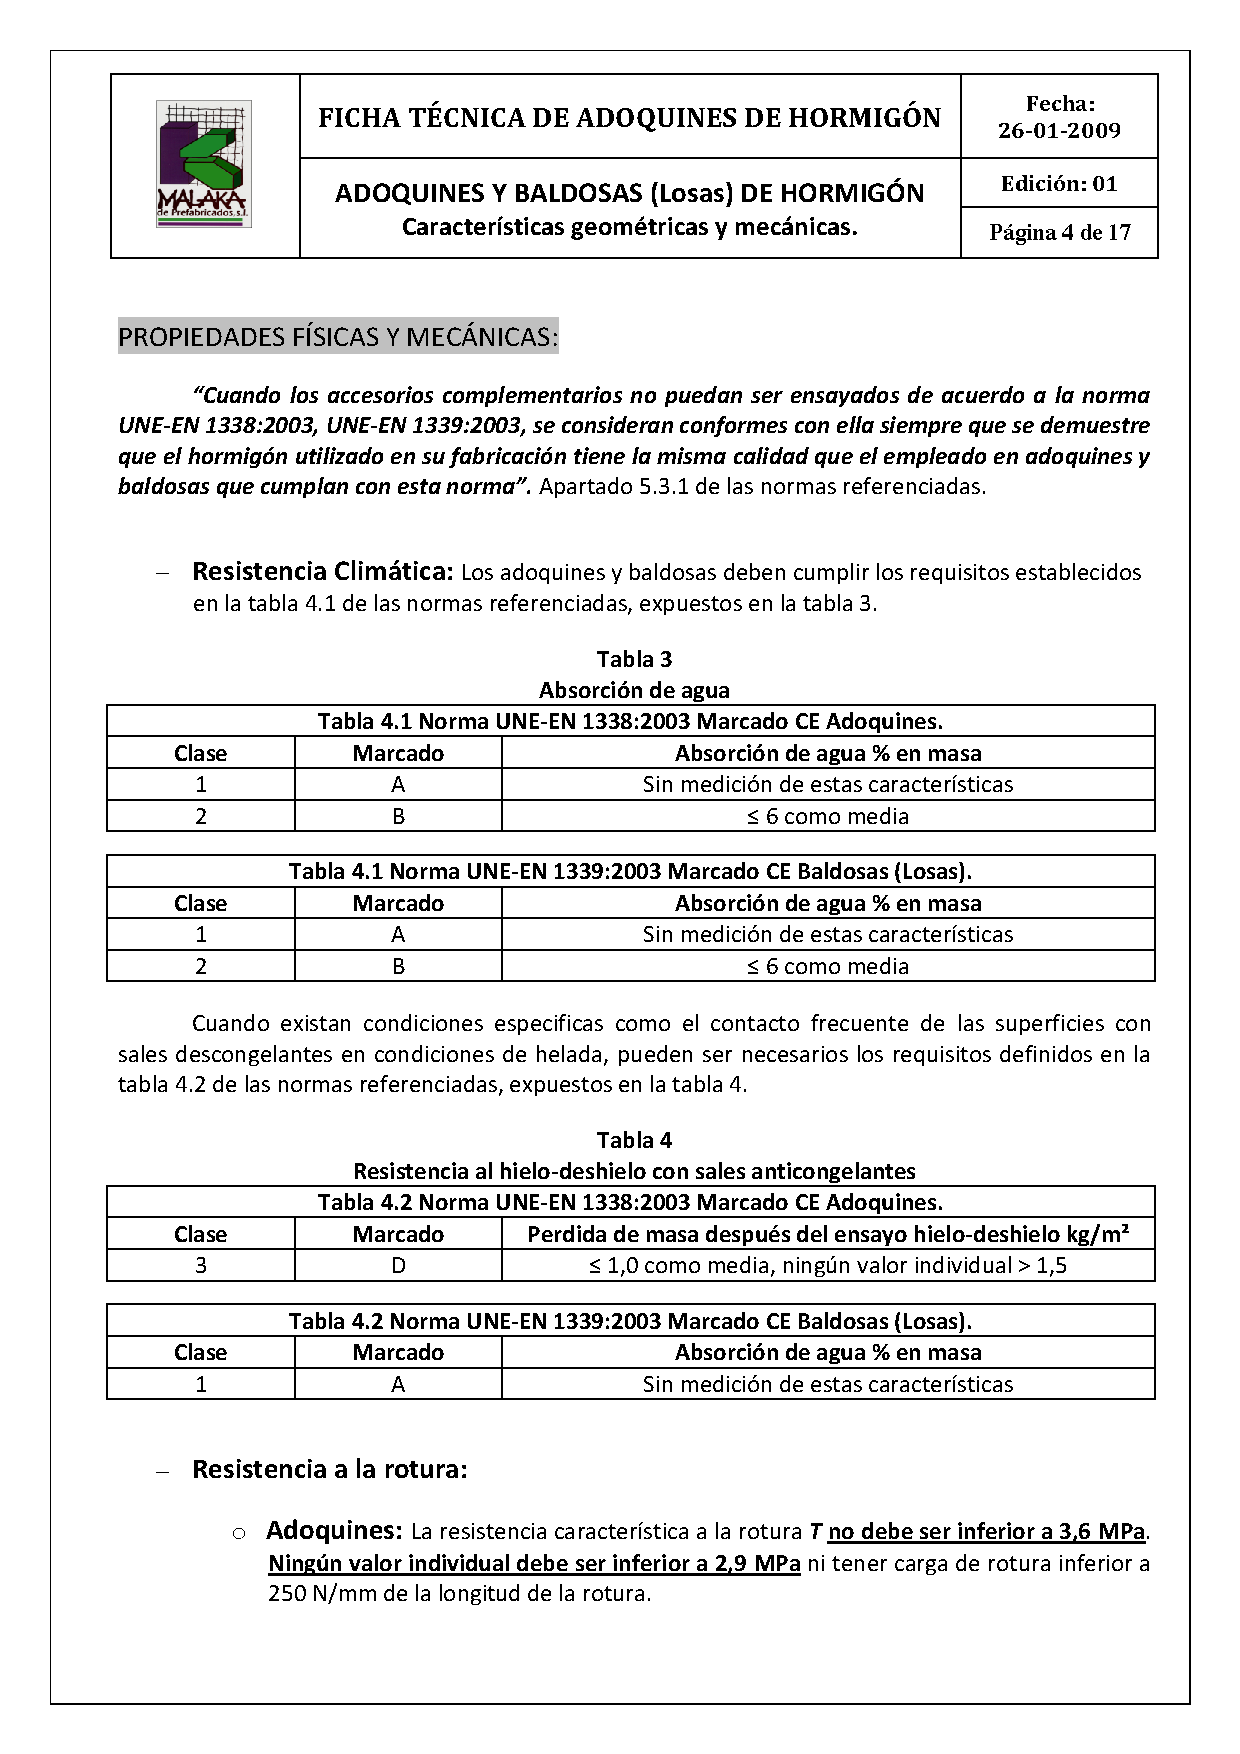
\includegraphics[scale=0.68]{ficha_tecnica/ft_adoquin_4.pdf}
\label{fig:ftadoquin4}
\end{figure}
\newpage
\begin{figure}[!htb]
\centering
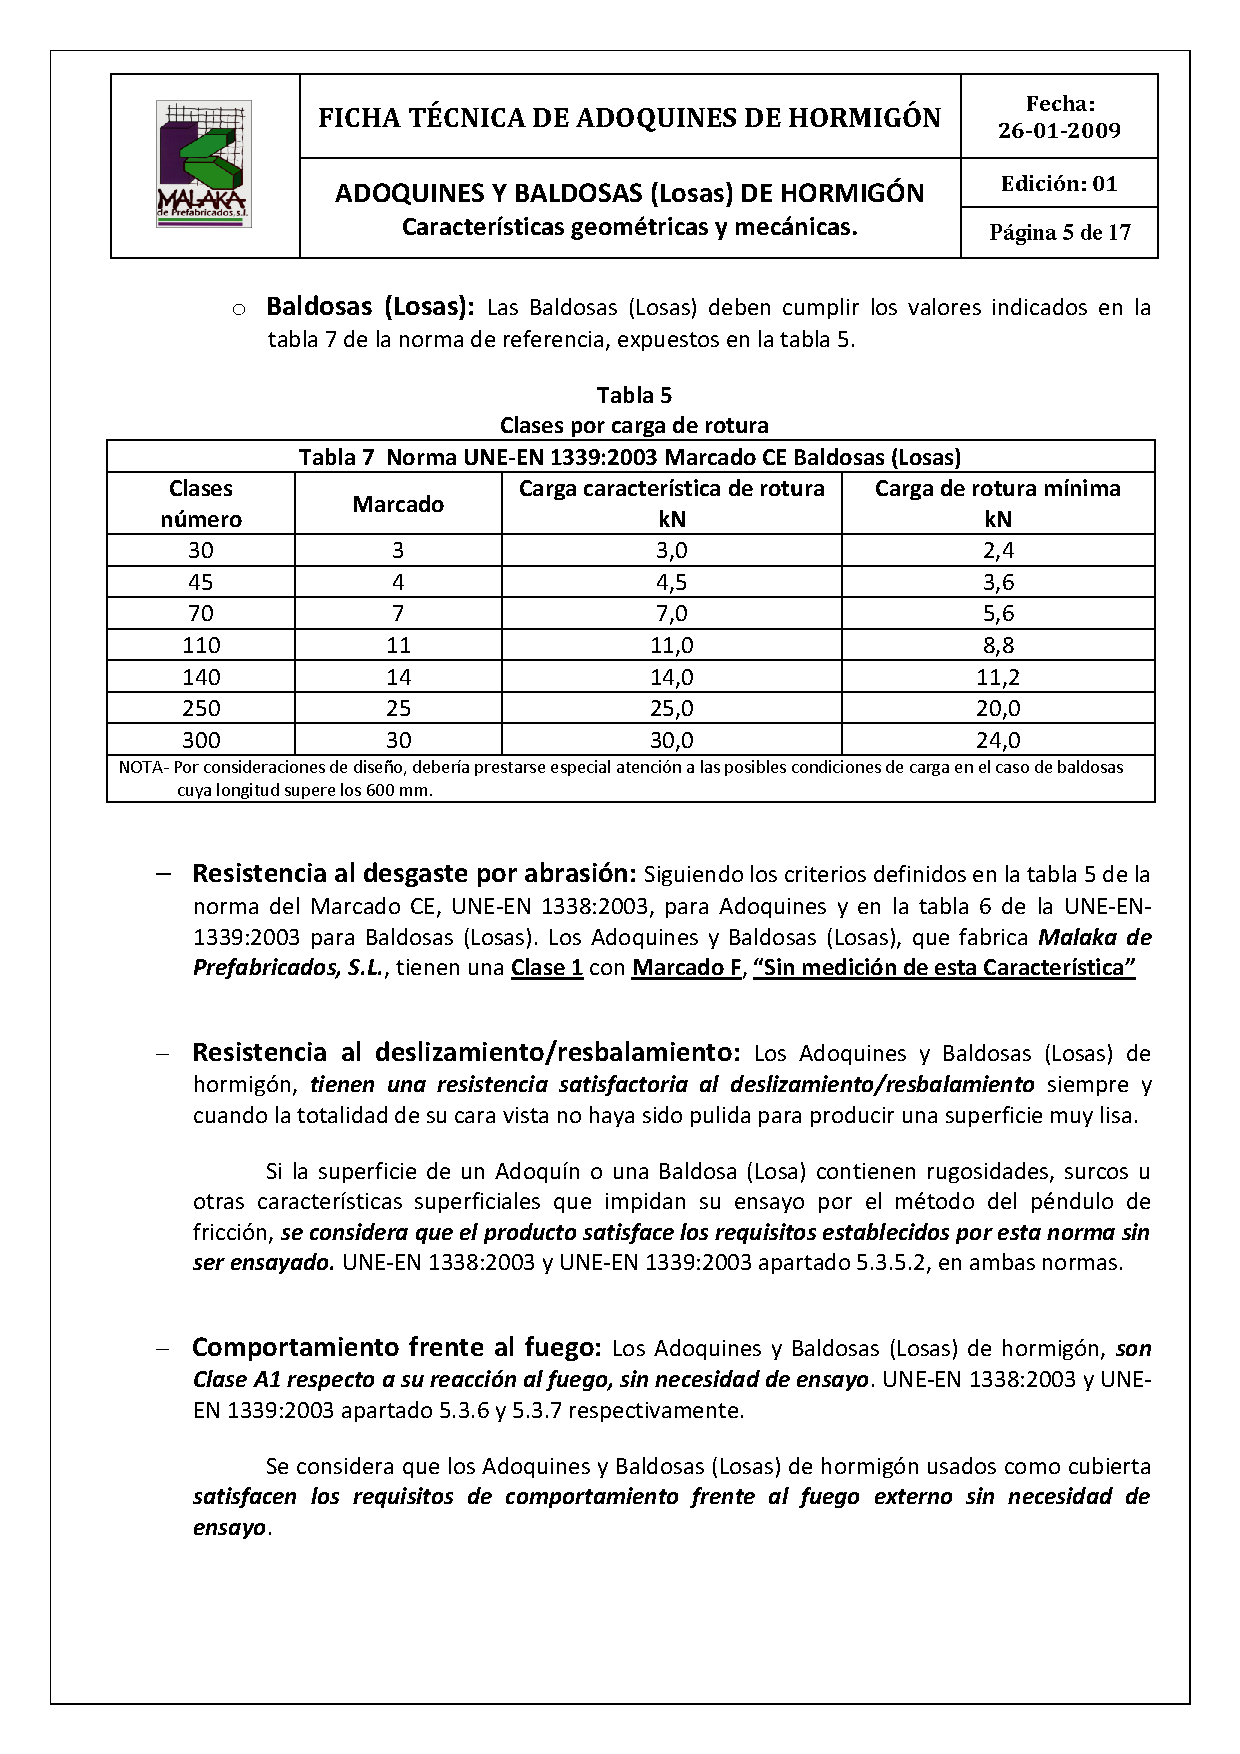
\includegraphics[scale=0.68]{ficha_tecnica/ft_adoquin_5.pdf}
\label{fig:ftadoquin5}
\end{figure}
\newpage
\begin{figure}[!htb]
\centering
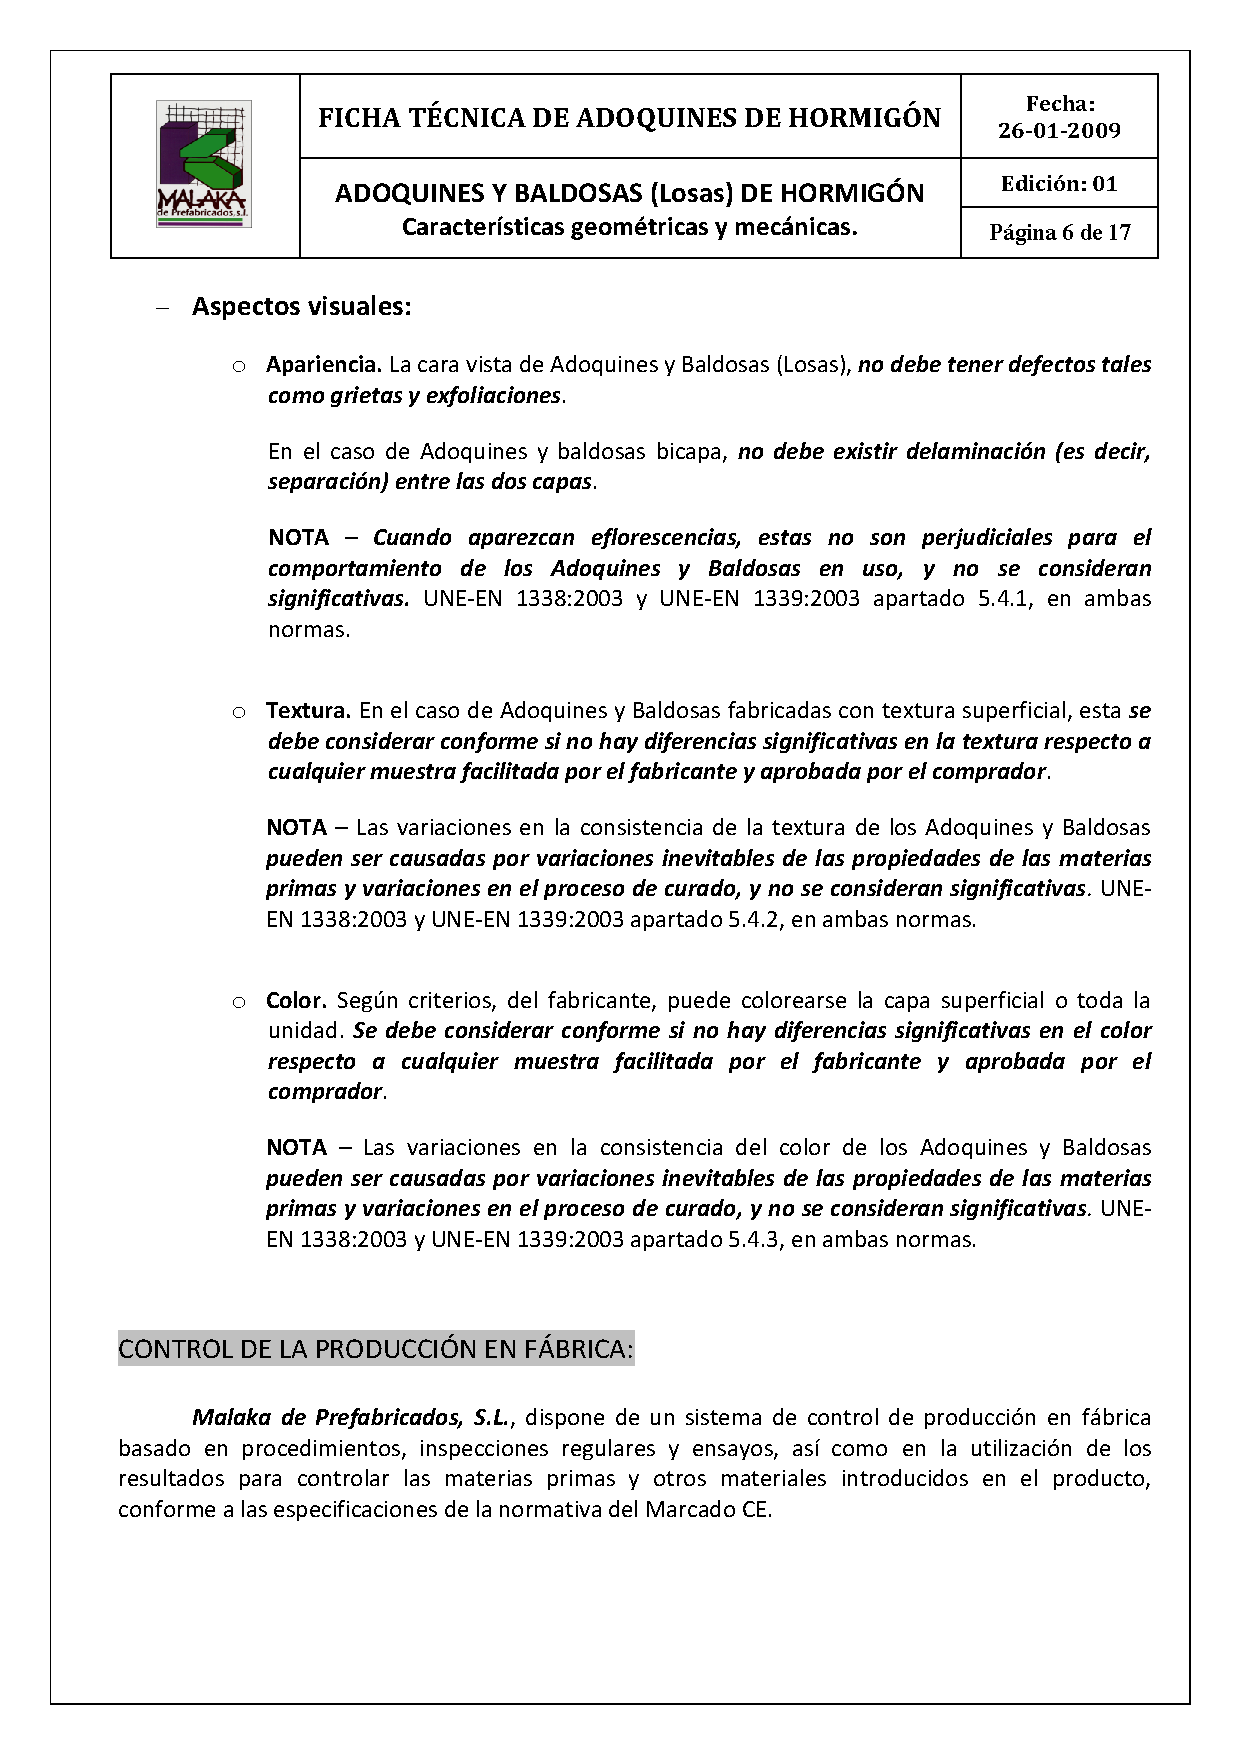
\includegraphics[scale=0.68]{ficha_tecnica/ft_adoquin_6.pdf}
\label{fig:ftadoquin6}
\end{figure}

\cleardoublepage
%!TEX root = informe.tex
\chapter{Herramientas utilizadas}\label{apend:herramientas}

Este proyecto ha sido tipografiado con el sistema de composición de documentos Xe\LaTeX. \LaTeX\ y Xe\LaTeX\ son distribuidos con el Mac\TeX, una redistribución de \TeX\ Live para OS X. La bibliografía ha sido generada mediante el sistema de gestión de referencias Bib\TeX.

Para la redacción se ha utilizado el editor de texto Sublime Text con el paquete LaTeXTools para la automatización de macros. Las fuentes de impresión empleadas son Minion Pro y Myriad Pro de Adobe.

Se ha utilizado un ordenador Apple Macbook Pro con sistema operativo OS X.

La generación de diagramas se ha realizado con MindNode para Mac y los paquetes de programación TikZ y PGF para Xe\LaTeX.

El software de Análisis de Ciclo de Vida elegido es SimaPro de PRé Consultants.

Los planos han sido creados usando el programa AutoCAD de Autodesk.

Las copias de seguridad se han realizado con el software de control de versiones Git en un repositorio online de Github y soporte local con Time Machine de Apple.

\cleardoublepage
\end{appendices}

\part{Planos}\label{planos}
%!TEX root = informe.tex
\setcounter{chapter}{1}
\addcontentsline{toc}{chapter}{\protect\numberline{\thechapter}Plano modelo adoquín Holanda 6}

\begin{figure}[!htb]
\centering
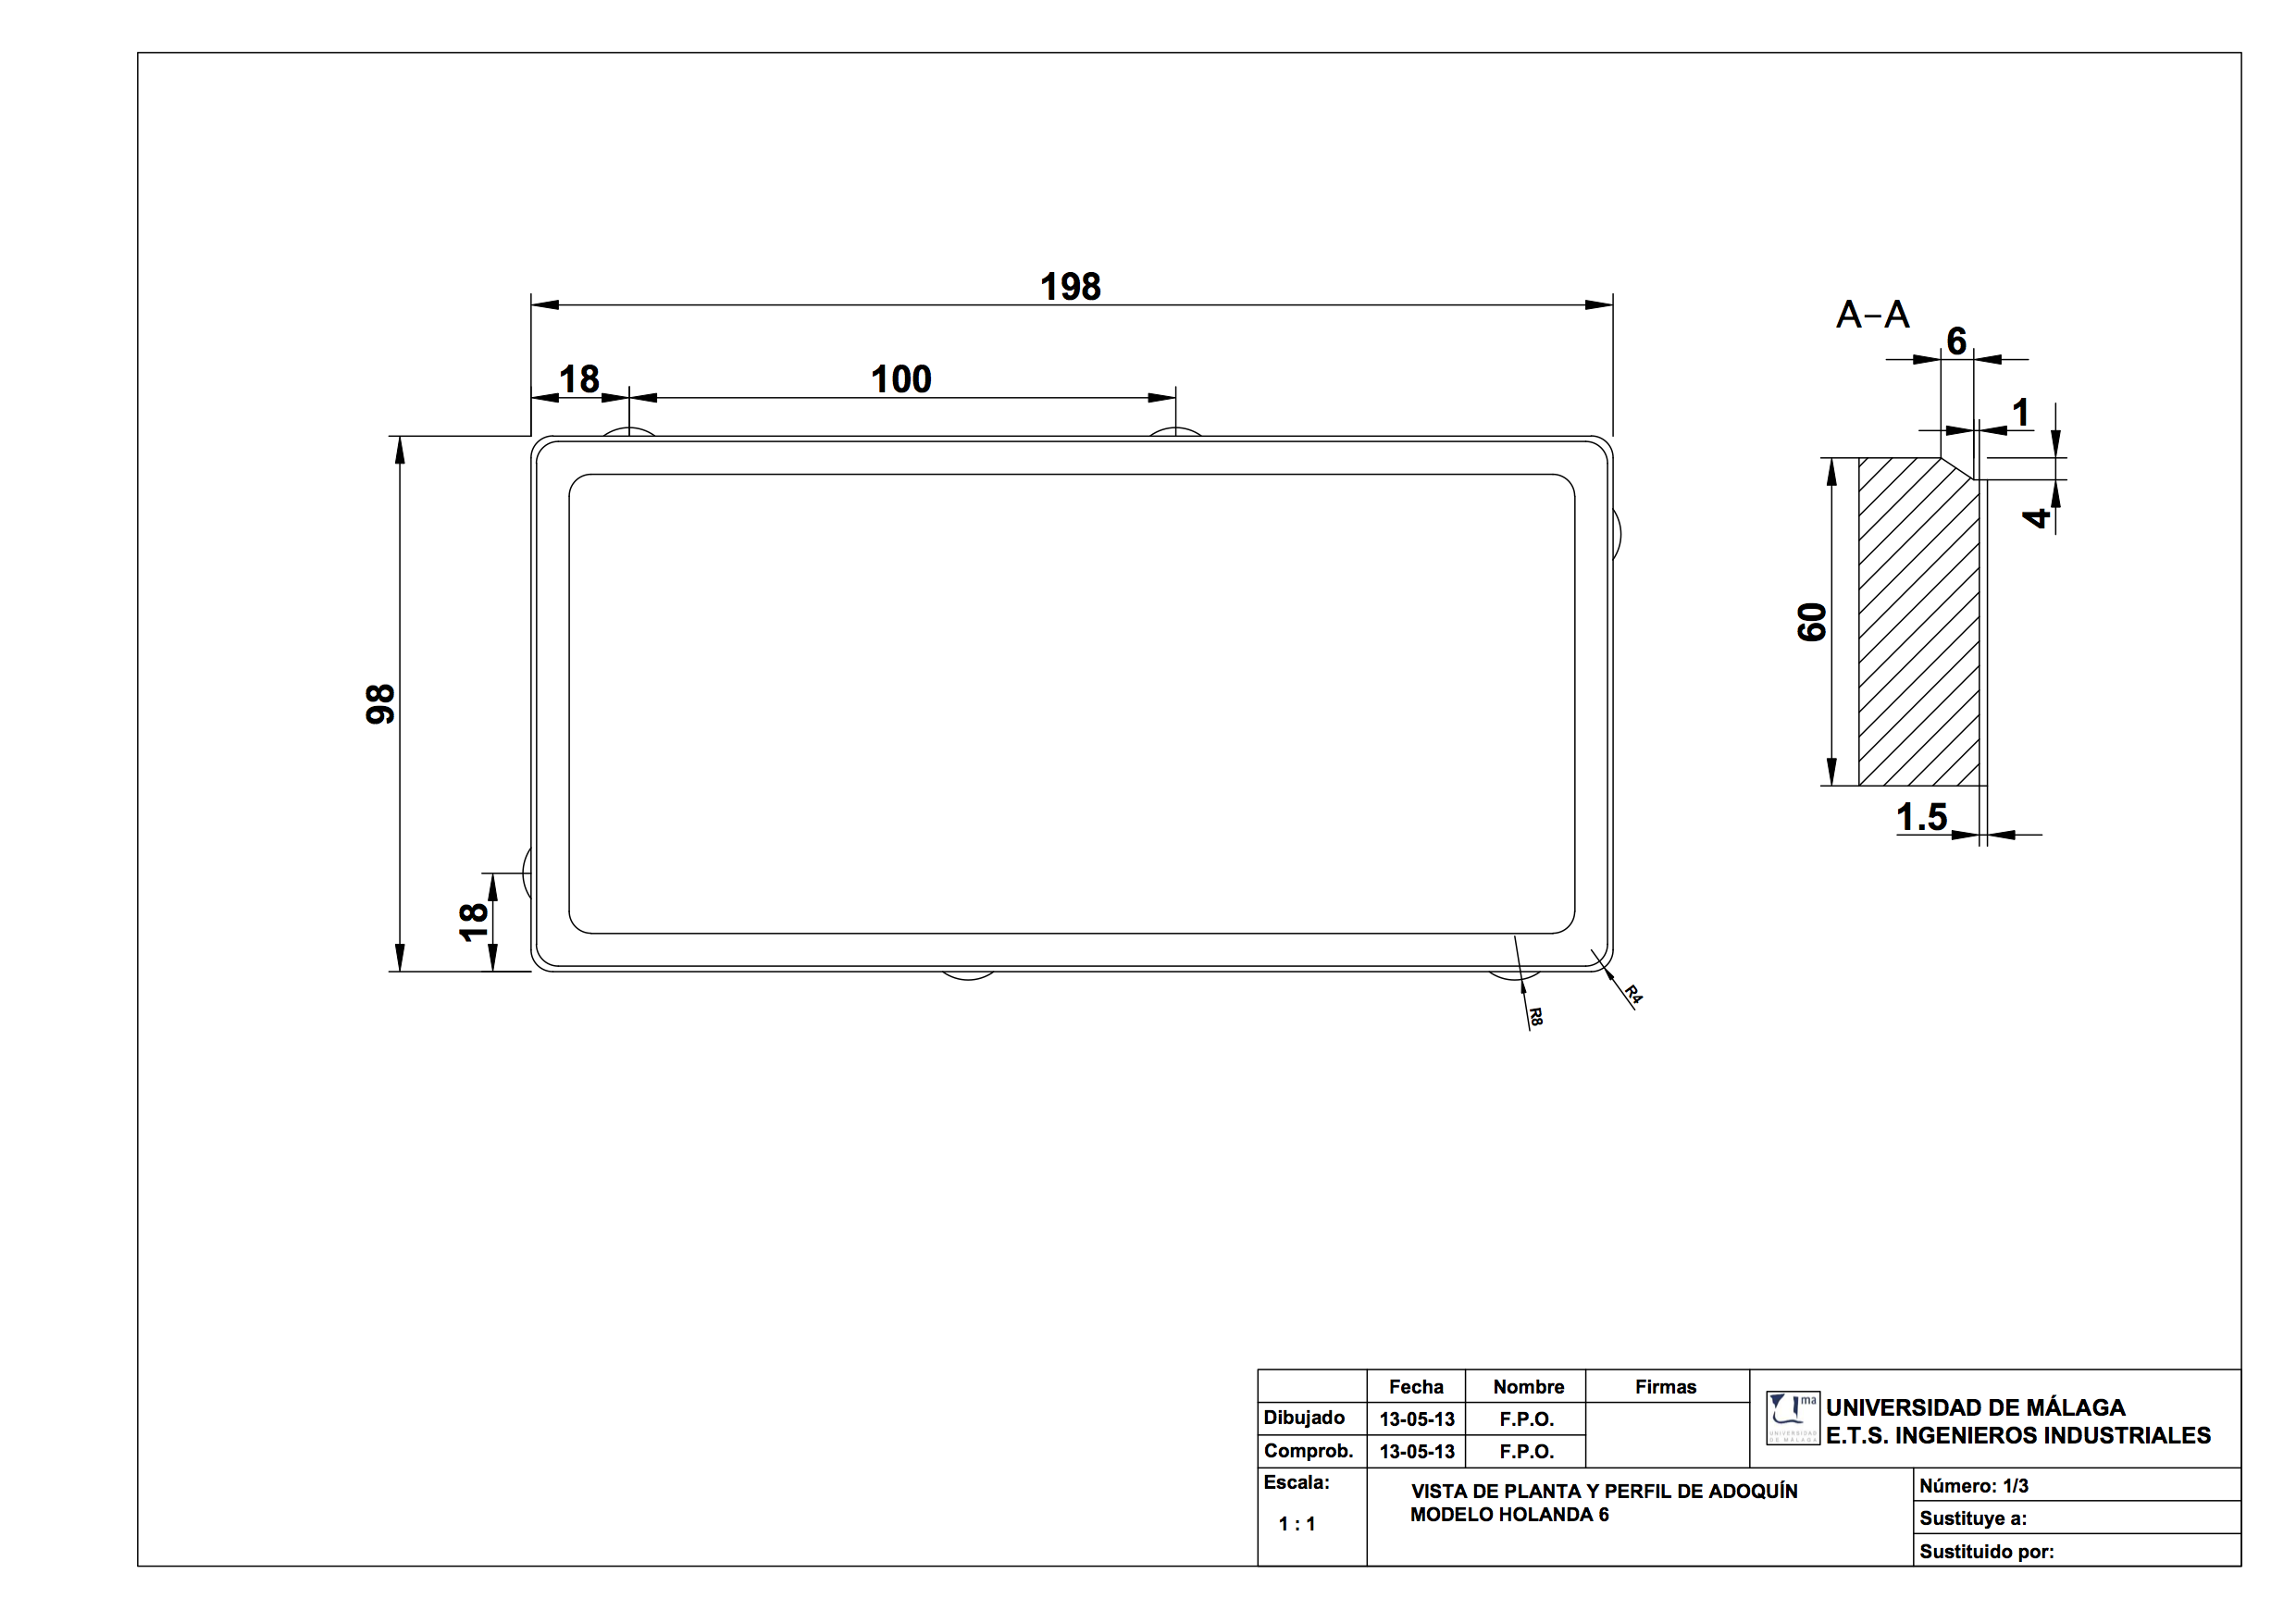
\includegraphics[angle=90,width=13.5cm]{plano_adoquin.png}
\end{figure}

\newpage
\setcounter{chapter}{2}
\addcontentsline{toc}{chapter}{\protect\numberline{\thechapter}Plano molde adoquín Holanda 6}
\begin{figure}[!htb]
\centering
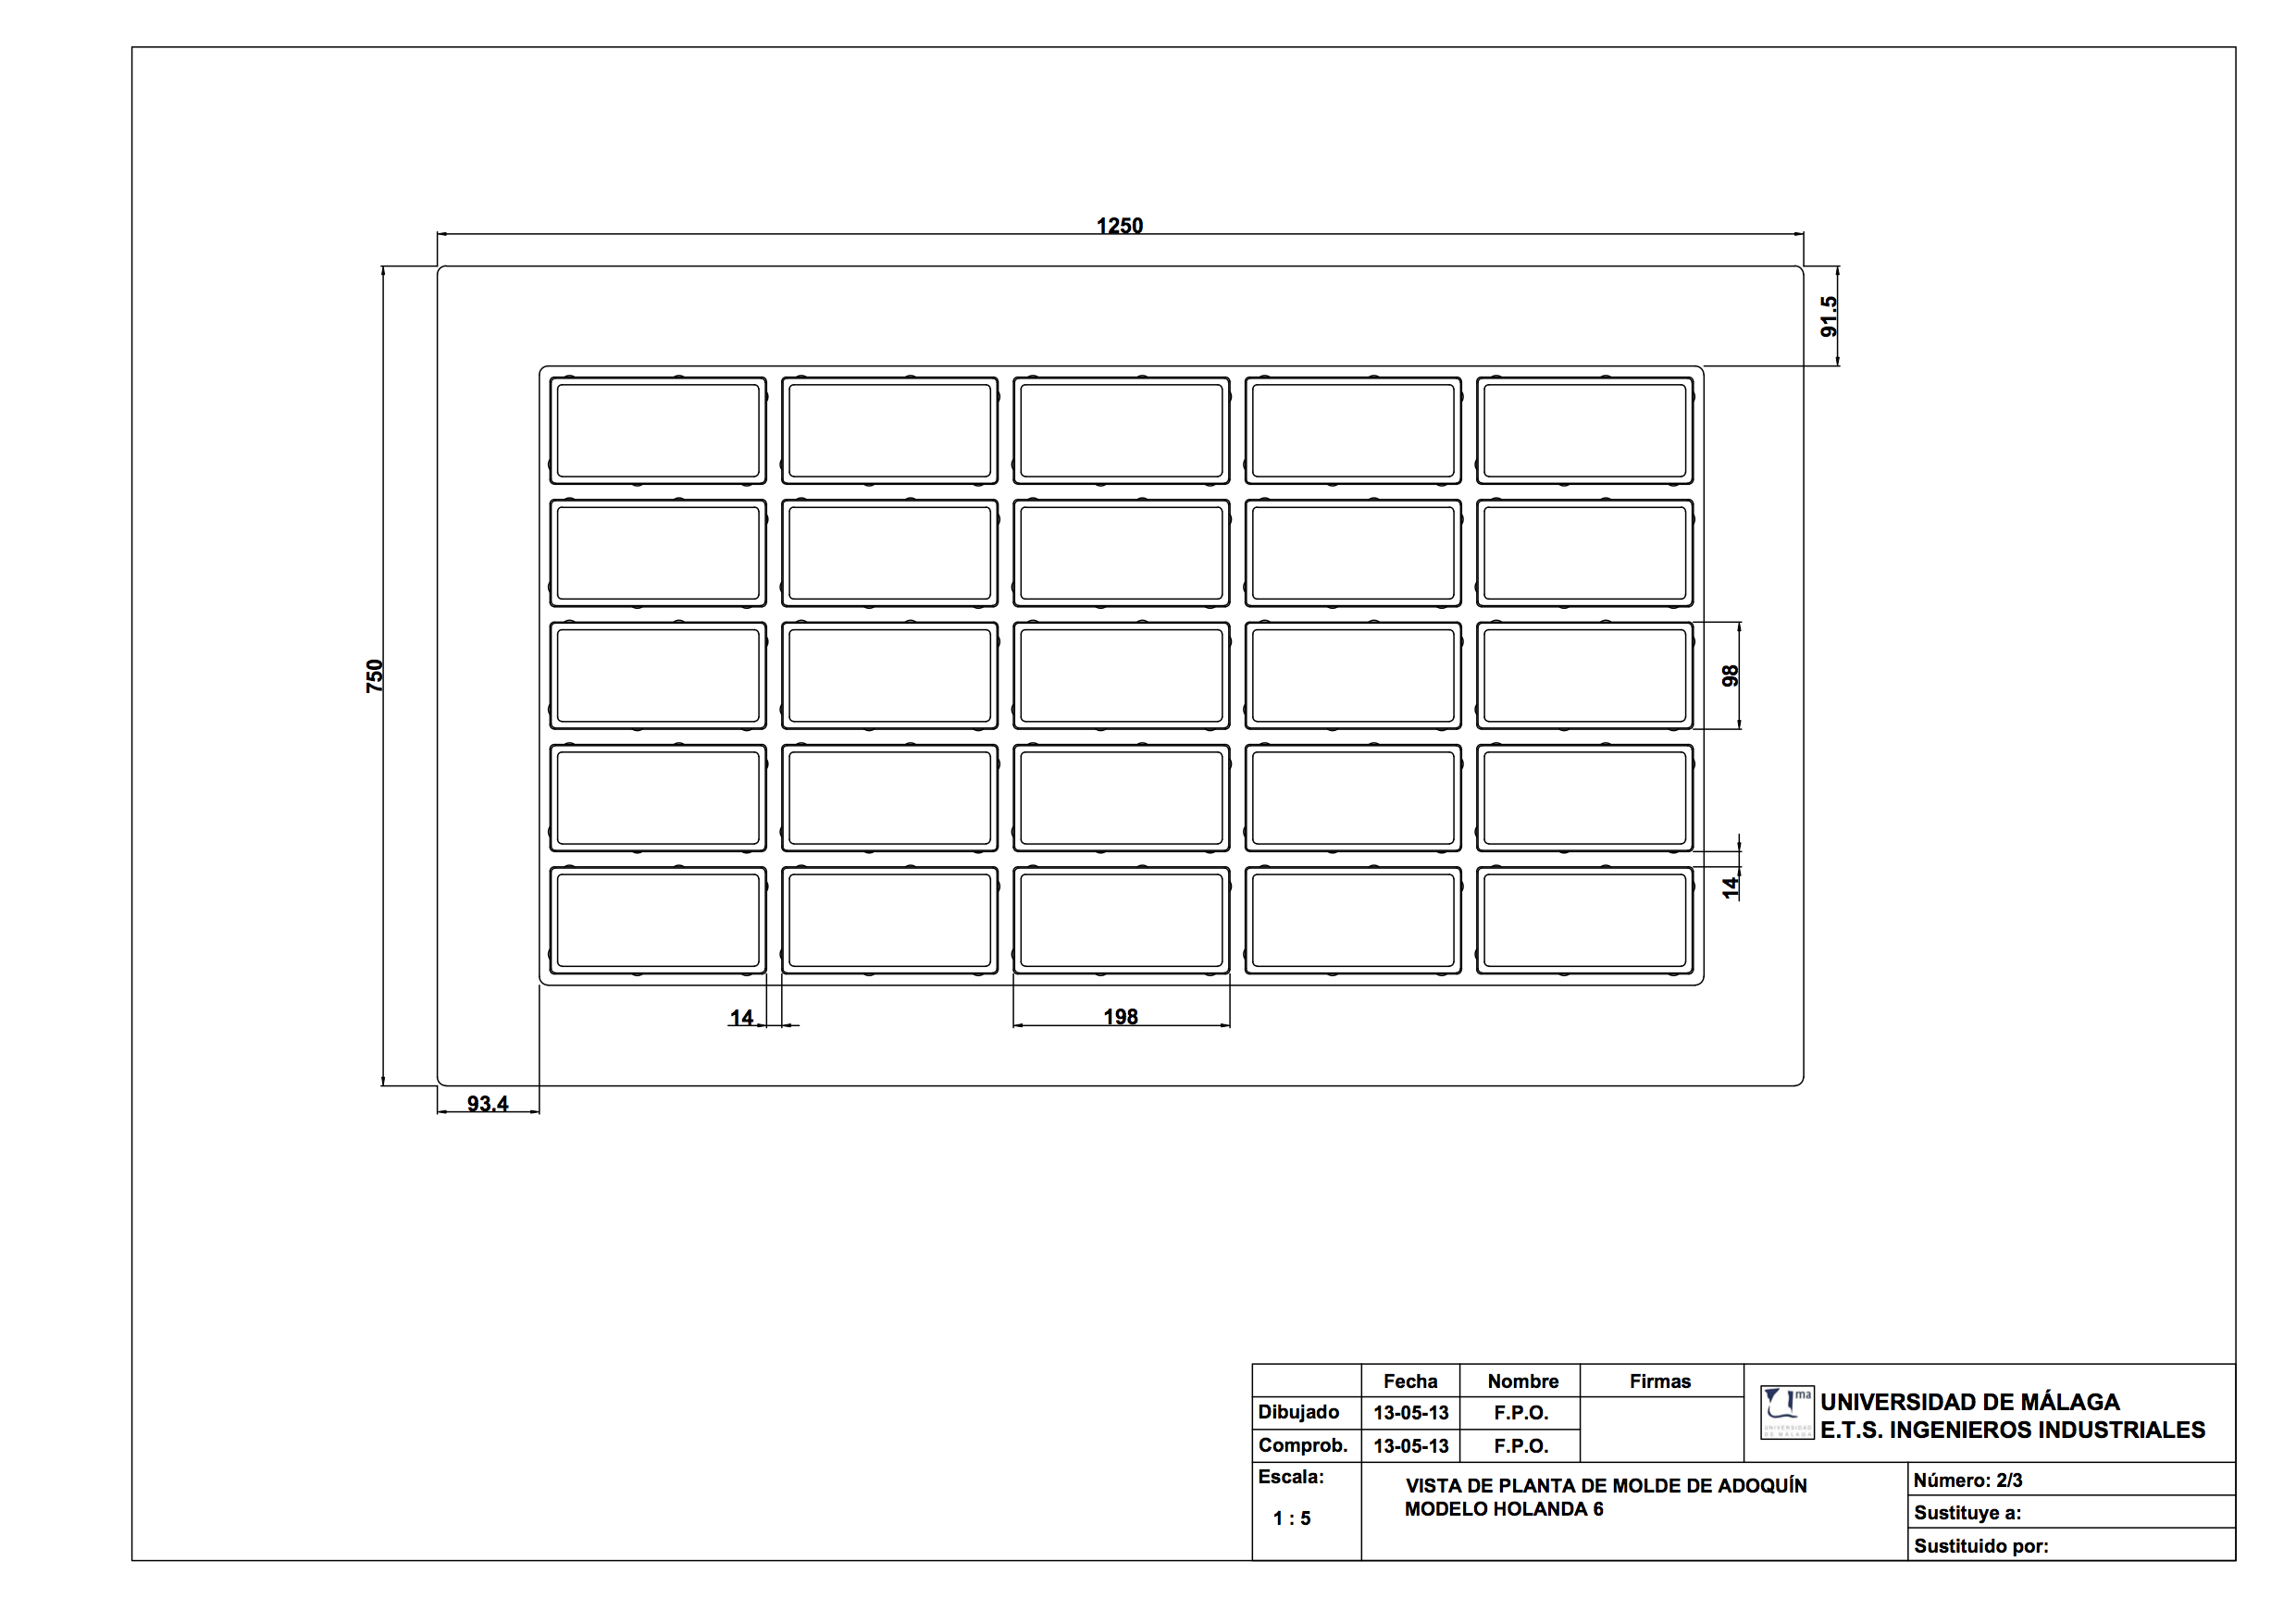
\includegraphics[angle=90,width=13.5cm]{plano_molde.png}
\end{figure}

\newpage
\setcounter{chapter}{3}
\addcontentsline{toc}{chapter}{\protect\numberline{\thechapter}Plano de instalaciones}
\begin{figure}[!htb]
\centering
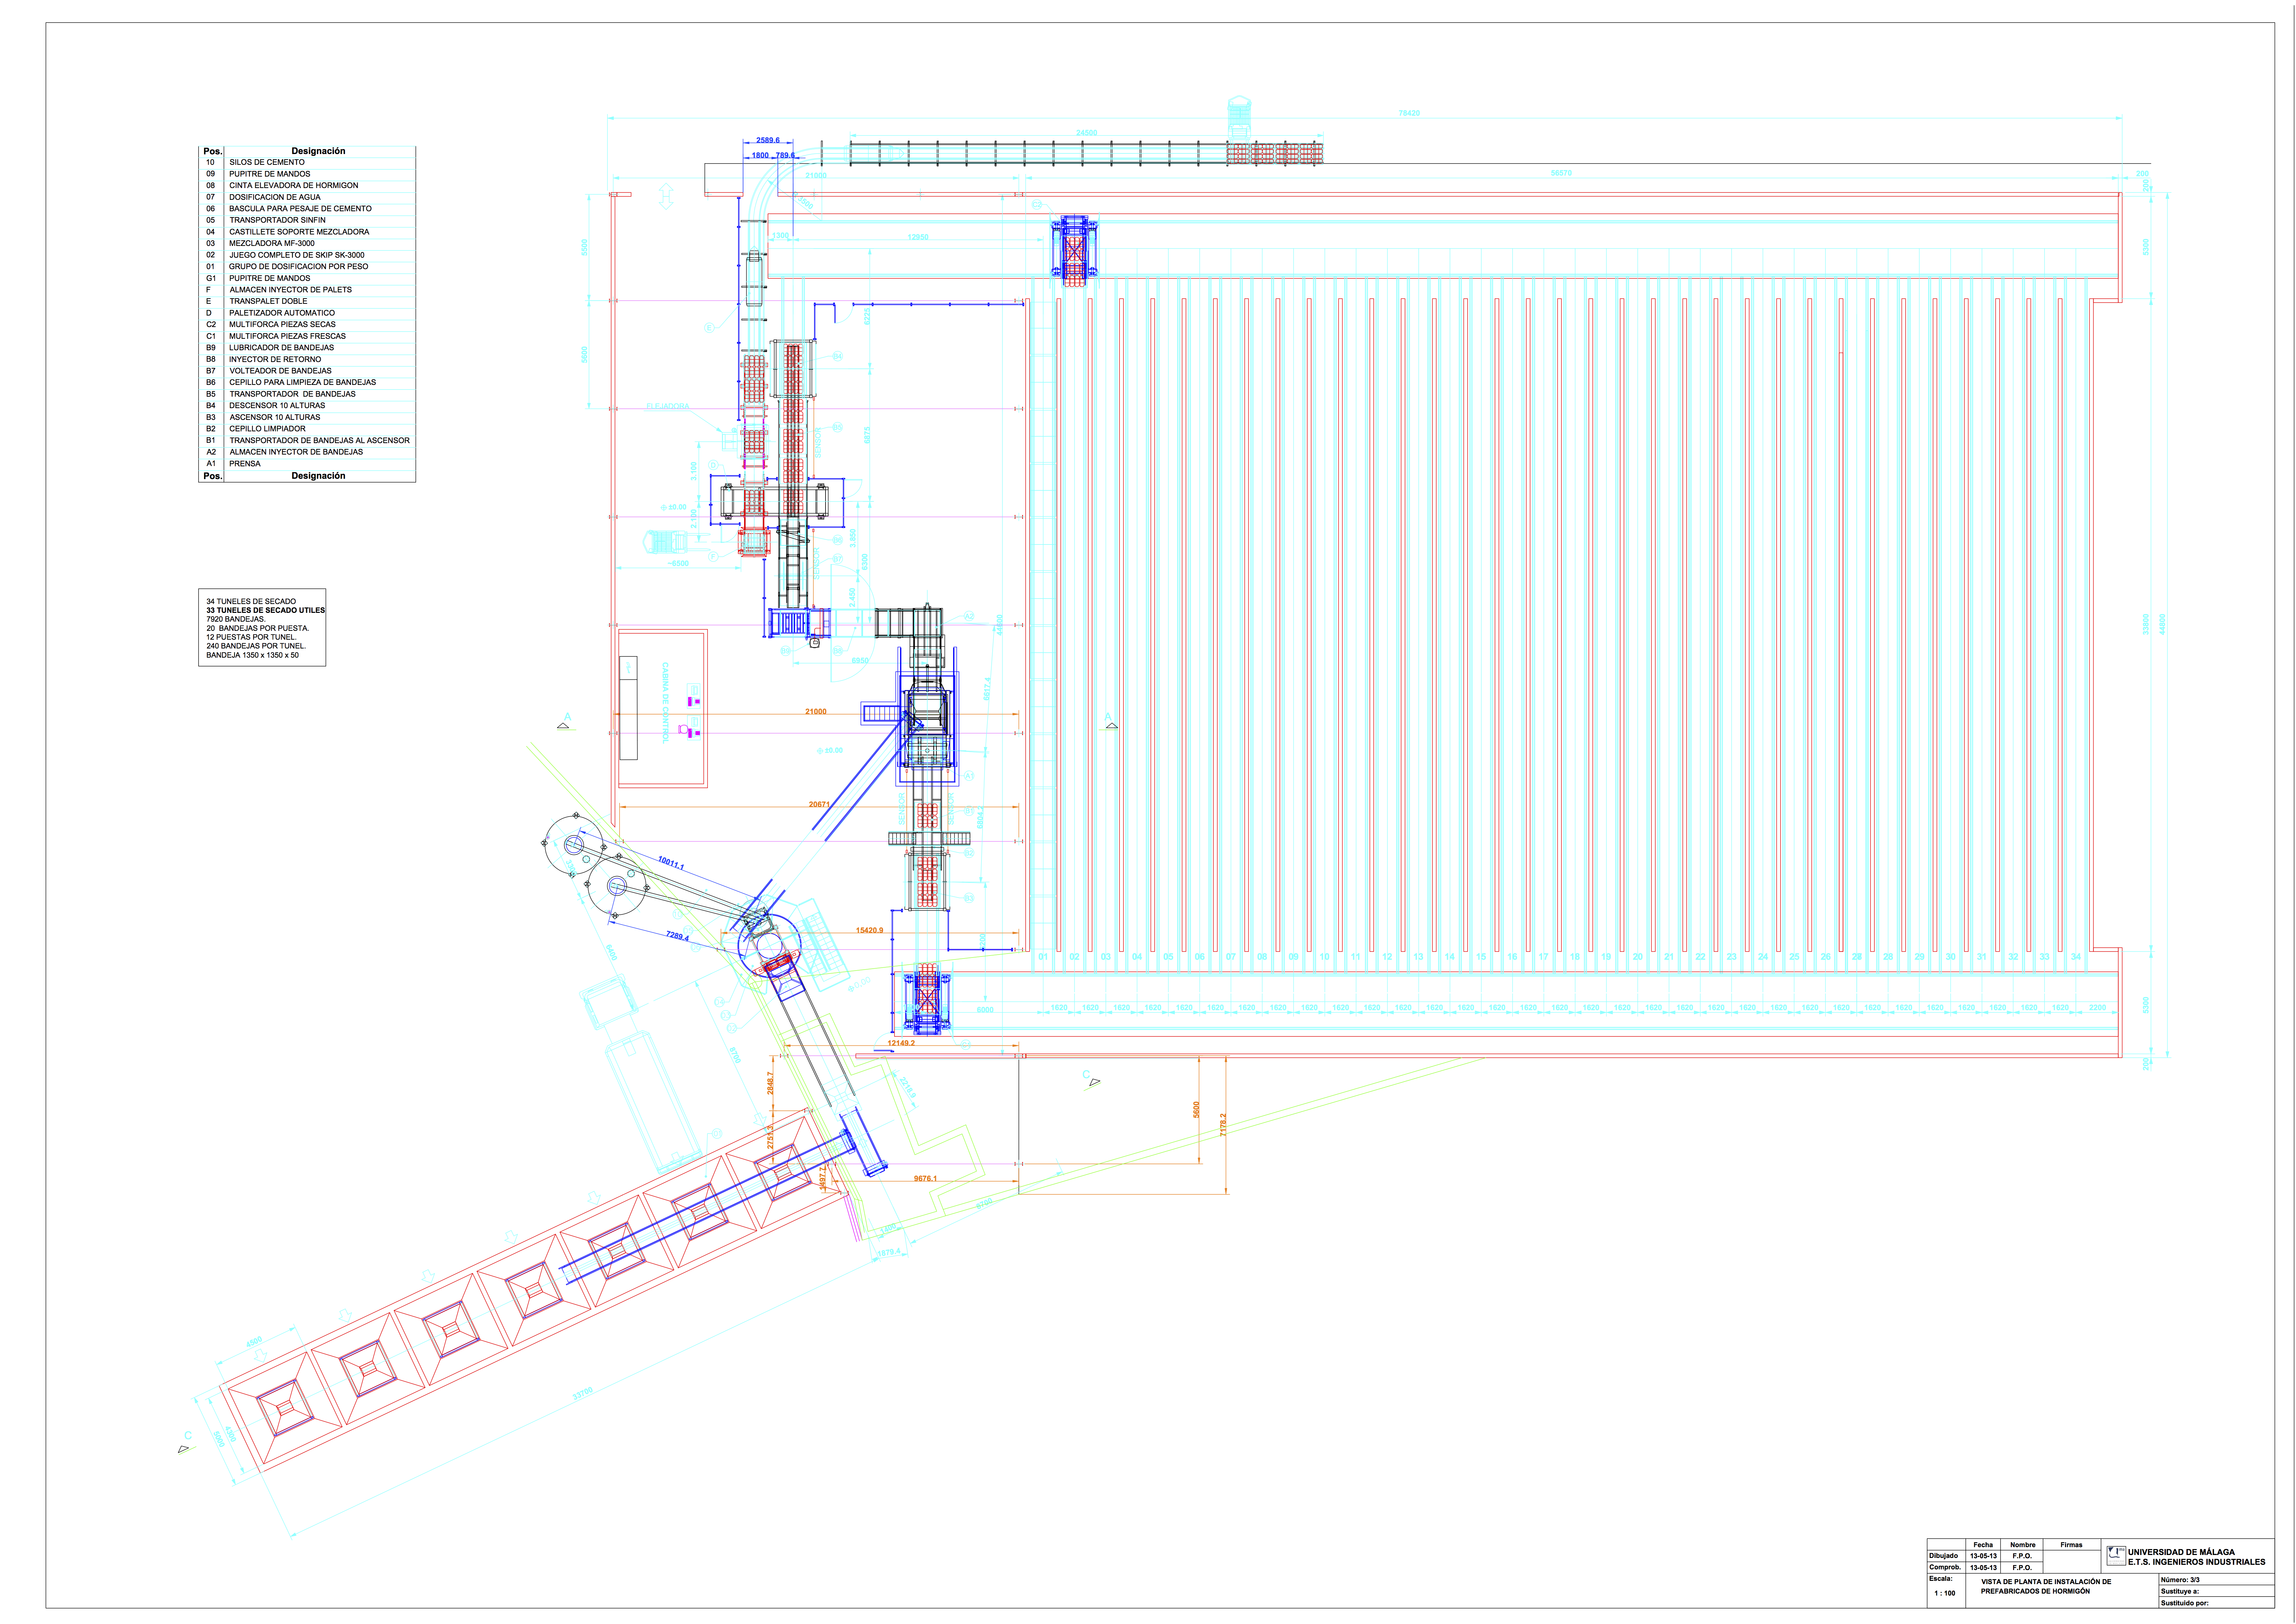
\includegraphics[angle=90,width=13.5cm]{plano_nave.png}
\end{figure}

\cleardoublepage

\part{Pliego de condiciones}
%!TEX root = informe.tex

\setcounter{chapter}{0}
\chapter{Condiciones técnicas}
% \addcontentsline{toc}{chapter}{Condiciones técnicas}

\section{Generalidades}

Los principios del Análisis de Ciclo de Vida son fundamentales y se deberán utilizar como orientación para tomar decisiones relacionadas tanto con la planificación como con la realización del análisis.

\section{Apreciación general del ciclo de vida}

El Análisis de Ciclo de Vida considerará el ciclo de vida completo del producto, desde la extracción y adquisición de la materia prima, pasando por la producción de energía y materia, y la fabricación, hasta el uso y el tratamiento al final de la vida útil y la disposición final. A través de esta visión general, se identificará y intentará evitar el desplazamiento de una carga ambiental potencial entre las etapas del ciclo de vida o los procesos individuales.

\section{Enfoque ambiental}
El Análisis de Ciclo de Vida tratará los aspectos e impactos ambientales del sistema del producto. Los aspectos e impactos económicos y sociales estarán fuera del alcance del Análisis de Ciclo de Vida. Se podrán combinar otras herramientas con el Análisis de Ciclo de Vida para análisis más profundos.

\section{Enfoque relativo y Unidad Funcional}
El Análisis de Ciclo de Vida será un enfoque relativo, que se estructurará alrededor de una Unidad Funcional. Esta Unidad Funcional definirá el estudio. Todos los análisis subsecuentes serán, por tanto, relativos a esa Unidad Funcional, ya que todas las entradas y salidas en el Inventario de Ciclo de Vida (ICV), y consecuentemente el perfil de la Evaluación del Impacto del Ciclo de Vida (EICV), se relacionarán con la Unidad Funcional.

\section{Enfoque iterativo}
El Análisis de Ciclo de Vida será una técnica iterativa. Las fases individuales del Análisis de Ciclo de Vida utilizarán resultados de las otras fases. El enfoque iterativo en y entre las fases contribuirá a la integridad y coherencia del estudio y de los resultados presentados.

\section{Transparencia}
Debido a la complejidad inherente al Análisis de Ciclo de Vida, la transparencia será un principio guía importante en la realización del Análisis de Ciclo de Vida, a fin de asegurar una adecuada interpretación de los resultados.

\section{Integridad}
El Análisis de Ciclo de Vida considerará todos los atributos o aspectos del entorno natural, de la salud humana y de los recursos. La consideración en un único estudio y con una perspectiva transversal de todos los atributos y aspectos, se podrán identificar y evaluar las compensaciones potenciales.

\section{Prioridad del enfoque científico}
Las decisiones en el Análisis de Ciclo de Vida se basarán preferentemente en las ciencias naturales. Si esto no es posible, se podrán utilizar otros enfoques, como las ciencias económicas y sociales, o se puede hacer referencia a convencio- nes internacionales. Si no existiera una base científica ni una justificación basada en otros enfoques o en convenciones internacionales, las decisiones se podrán basar en juicios de valor.

\section{Alcance}
Cuando se defina el alcance del Análisis de Ciclo de Vida, se considerará el contexto de la toma de decisión; es decir, los sistemas del producto estudiados deberán tratar adecuadamente los productos y procesos afectados por la aplicación prevista.

Los ejemplos de aplicación se referirán a decisiones que pretendan conseguir mejoras ambientales, lo que también constituye el enfoque global de la serie ISO 14000. Por lo tanto, los productos y procesos estudiados en un Análisis de Ciclo de Vida son aquellos afectados por la decisión que el Análisis de Ciclo de Vida pretende apoyar.

\chapter{Condiciones administrativas y legales}
% \addcontentsline{toc}{chapter}{Condiciones administrativas y legales}

\section{Autoría}
El autor de este proyecto cede al 50\% los derechos derivados de este proyecto al Departamento de Expresión Gráfica, Diseño y Proyectos de la Escuela Técnica Superior de Ingeniería Industrial de la Universidad de Málaga.

\section{Realización y supervisión}
El presente proyecto será realizado por el autor del mismo, bajo dirección y supervisión del tutor. Si esto no fuera posible, dicha realización y asesoría debería ser llevada a cabo por personal del Departamento de Expresión Gráfica, Diseño y Proyectos de la Escuela Técnica Superior de Ingeniería Industrial de la Universidad de Málaga.

\section{Cambios y desarrollos posteriores}
El autor del presente proyecto deberá ser puntualmente informado de los posibles cambios o modificaciones que pudiesen realizarse en el mismo.

En el caso de cambios o desarrollos posteriores de este proyecto se informará al autor para colaborar en el estudio o investigación que se este realizando.

\section{Consultas}
Se autoriza la consulta de este proyecto a toda persona autorizada por parte del Departamento de Expresión Gráfica, Diseño y Proyectos y a cualquier persona matriculada en la Universidad de Málaga que podrá solicitar el Proyecto en la Biblioteca de la Escuela Técnica Superior de Ingeniería Industrial de la Universidad de Málaga.

\vspace{1cm}
\today \hfill Fdo. Francisco José Pinto Oliver

\cleardoublepage

\part{Presupuesto}
%!TEX root = informe.tex
\chapter*{Coste de materiales}
\addcontentsline{toc}{chapter}{Coste de materiales}
Se contabilizarán todos los costes —en euros— relacionados con recursos materiales tales como material de oficina, software y hardware informático.

Respecto al material de oficina, abarca desde el soporte en papel para la impresión de documentación, fotocopias, encuadernación de este proyecto, soporte óptico que acompaña a este proyecto, planos hasta los cartuchos de tinta para su impresión.

El apartado de equipo informático engloba una licencia de sistema operativo, un procesador de textos para la redacción del presente proyecto, software para la creación de diagramas de flujo y tratamiento de imágenes.

En cuanto al software informático, se ha incluido una licencia para un único usuario tipo analista válida indefinidamente. Esto incluye el precio de la base de datos \textit{ecoinvent} versión 2 y la actualización a la versión 3. También incluye un año gratuito de soporte online y actualizaciones.

\begin{table}[!htb]
\centering
\begin{tabular}{lcrr}
\toprule
\multicolumn{4}{c}{Coste de materiales}\\
\midrule
Concepto & Cantidad & Importe (\euro) & Total (\euro)\\
\midrule
\multicolumn{2}{c}{Licencia SimaPro}\\
\cmidrule(r){1-2}
SimaPro single user, indefinite, Analyst & 1 & 8800.00 & 8800.00\\
ecoinvent Database & 1 & 0.00 & 0.00\\
Soporte y actualizaciones (1 año) & 1 & 0.00 & 0.00\\
\multicolumn{2}{c}{Equipo informático}\\
\cmidrule(r){1-2}
Ordenador portátil & 1 & 1329.00 & 1329.00\\
Procesador de texto & 1 & 0.00 & 0.00\\
Hoja de cálculo & 1 & 8.99 & 8.99\\
Software diagramas & 1 & 0.00 & 0.00\\
\multicolumn{2}{c}{Material de oficina}\\
\cmidrule(r){1-2}
DIN-A4 (500 uds.) & 1 & 5.50 & 5.50\\
Cartucho tinta negra & 1 & 18.00 & 18.00\\
Cartucho tinta color & 1 & 23.00 & 23.00\\
Encuadernación de tornillo & 1 & 12.00 & 12.00\\
Disco óptico DVD-R & 3 & 0.50 & 1.50\\
\bottomrule
Subtotal materiales & & & 10197.99\\
\bottomrule
\end{tabular}
% \caption{Presupuesto de materiales.}
\label{presupuestomateriales}
\end{table}

\chapter*{Coste de desarrollo}
\addcontentsline{toc}{chapter}{Coste de desarrollo}
El coste de desarrollo abarca los recursos humanos —en horas— necesarios para la realización del presente proyecto, documentación, recopilación de datos, redacción y correcciones del proyecto.

\begin{table}[!htb]
\centering
\begin{tabular}{lcrr}
\toprule
\multicolumn{4}{c}{Coste de desarrollo}\\
\midrule
Concepto & Cantidad (h) & Importe (\euro) & Total (\euro)\\
\midrule
\multicolumn{2}{c}{Documentación}\\
\cmidrule(r){1-2}
Documentación & 130 & 19.00 & 8800.00\\
Entrevista con fabricante & 17 & 19.00 & 0.00\\
Consultas varias & 11 & 19.00 & 0.00\\
\multicolumn{2}{c}{Redacción del proyecto}\\
\cmidrule(r){1-2}
Redacción & 170 & 19.00 & 5.50\\
Introducción del modelado & 60 & 19.00 & 18.00\\
Corrección de errores & 35 & 19.00 & 23.00\\
\bottomrule
Subtotal desarrollo & & & 8037.00\\
\bottomrule
\end{tabular}
% \caption{Presupuesto de desarrollo.}
\label{presupuestodesarrollo}
\end{table}

\chapter*{Presupuesto general}
\addcontentsline{toc}{chapter}{Presupuesto general}

\begin{table}[!htb]
\centering
\begin{tabular}{lcrr}
\toprule
\multicolumn{4}{c}{Coste total del proyecto}\\
\midrule
Concepto & Cantidad & Importe (\euro) & Total (\euro)\\
\midrule
Subtotal materiales & & & 10197.99\\
Subtotal desarrollo & & & 8037.00\\
\bottomrule
Total & & & 18234.99\\
\bottomrule
\end{tabular}
% \caption{Coste total del proyecto.}
\label{presupuestototal}
\end{table}

\begin{table}[!htb]
\centering
\begin{tabular}{lcrr}
\toprule
\multicolumn{4}{c}{Presupuesto general}\\
\midrule
Concepto & Cantidad (\%) & Importe (\euro) & Total (\euro)\\
\midrule
Coste total del proyecto & & & 18234.99\\
Gastos generales & 13 & & 2370.55\\
Beneficio industrial & 6 & & 1094.10\\
I.V.A. & 21 & & 3829.35\\
\bottomrule
Total & & & 25528.99\\
\bottomrule
\end{tabular}
% \caption{Presupuesto general.}
\label{presupuestogeneral}
\end{table}

\end{document}
